% Options for packages loaded elsewhere
\PassOptionsToPackage{unicode}{hyperref}
\PassOptionsToPackage{hyphens}{url}
%
\documentclass[
  letterpaper,
]{scrbook}

\usepackage{amsmath,amssymb}
\usepackage{iftex}
\ifPDFTeX
  \usepackage[T1]{fontenc}
  \usepackage[utf8]{inputenc}
  \usepackage{textcomp} % provide euro and other symbols
\else % if luatex or xetex
  \usepackage{unicode-math}
  \defaultfontfeatures{Scale=MatchLowercase}
  \defaultfontfeatures[\rmfamily]{Ligatures=TeX,Scale=1}
\fi
\usepackage{lmodern}
\ifPDFTeX\else  
    % xetex/luatex font selection
\fi
% Use upquote if available, for straight quotes in verbatim environments
\IfFileExists{upquote.sty}{\usepackage{upquote}}{}
\IfFileExists{microtype.sty}{% use microtype if available
  \usepackage[]{microtype}
  \UseMicrotypeSet[protrusion]{basicmath} % disable protrusion for tt fonts
}{}
\makeatletter
\@ifundefined{KOMAClassName}{% if non-KOMA class
  \IfFileExists{parskip.sty}{%
    \usepackage{parskip}
  }{% else
    \setlength{\parindent}{0pt}
    \setlength{\parskip}{6pt plus 2pt minus 1pt}}
}{% if KOMA class
  \KOMAoptions{parskip=half}}
\makeatother
\usepackage{xcolor}
\usepackage[paper=a4paper,top=2cm,bottom=2cm,left=1.5cm,right=3.5cm,marginparwidth=2.5cm,marginparsep=2.5mm,twoside]{geometry}
\setlength{\emergencystretch}{3em} % prevent overfull lines
\setcounter{secnumdepth}{5}
% Make \paragraph and \subparagraph free-standing
\ifx\paragraph\undefined\else
  \let\oldparagraph\paragraph
  \renewcommand{\paragraph}[1]{\oldparagraph{#1}\mbox{}}
\fi
\ifx\subparagraph\undefined\else
  \let\oldsubparagraph\subparagraph
  \renewcommand{\subparagraph}[1]{\oldsubparagraph{#1}\mbox{}}
\fi

\usepackage{color}
\usepackage{fancyvrb}
\newcommand{\VerbBar}{|}
\newcommand{\VERB}{\Verb[commandchars=\\\{\}]}
\DefineVerbatimEnvironment{Highlighting}{Verbatim}{commandchars=\\\{\}}
% Add ',fontsize=\small' for more characters per line
\usepackage{framed}
\definecolor{shadecolor}{RGB}{243,245,246}
\newenvironment{Shaded}{\begin{snugshade}}{\end{snugshade}}
\newcommand{\AlertTok}[1]{\textcolor[rgb]{1.00,0.00,0.00}{\textbf{#1}}}
\newcommand{\AnnotationTok}[1]{\textcolor[rgb]{0.38,0.63,0.69}{\textbf{\textit{#1}}}}
\newcommand{\AttributeTok}[1]{\textcolor[rgb]{0.49,0.56,0.16}{#1}}
\newcommand{\BaseNTok}[1]{\textcolor[rgb]{0.25,0.63,0.44}{#1}}
\newcommand{\BuiltInTok}[1]{\textcolor[rgb]{0.00,0.50,0.00}{#1}}
\newcommand{\CharTok}[1]{\textcolor[rgb]{0.25,0.44,0.63}{#1}}
\newcommand{\CommentTok}[1]{\textcolor[rgb]{0.38,0.63,0.69}{\textit{#1}}}
\newcommand{\CommentVarTok}[1]{\textcolor[rgb]{0.38,0.63,0.69}{\textbf{\textit{#1}}}}
\newcommand{\ConstantTok}[1]{\textcolor[rgb]{0.53,0.00,0.00}{#1}}
\newcommand{\ControlFlowTok}[1]{\textcolor[rgb]{0.00,0.44,0.13}{\textbf{#1}}}
\newcommand{\DataTypeTok}[1]{\textcolor[rgb]{0.56,0.13,0.00}{#1}}
\newcommand{\DecValTok}[1]{\textcolor[rgb]{0.25,0.63,0.44}{#1}}
\newcommand{\DocumentationTok}[1]{\textcolor[rgb]{0.73,0.13,0.13}{\textit{#1}}}
\newcommand{\ErrorTok}[1]{\textcolor[rgb]{1.00,0.00,0.00}{\textbf{#1}}}
\newcommand{\ExtensionTok}[1]{\textcolor[rgb]{0.00,0.44,0.13}{#1}}
\newcommand{\FloatTok}[1]{\textcolor[rgb]{0.25,0.63,0.44}{#1}}
\newcommand{\FunctionTok}[1]{\textcolor[rgb]{0.02,0.16,0.49}{#1}}
\newcommand{\ImportTok}[1]{\textcolor[rgb]{0.00,0.50,0.00}{\textbf{#1}}}
\newcommand{\InformationTok}[1]{\textcolor[rgb]{0.38,0.63,0.69}{\textbf{\textit{#1}}}}
\newcommand{\KeywordTok}[1]{\textcolor[rgb]{0.00,0.44,0.13}{\textbf{#1}}}
\newcommand{\NormalTok}[1]{\textcolor[rgb]{0.00,0.44,0.13}{#1}}
\newcommand{\OperatorTok}[1]{\textcolor[rgb]{0.40,0.40,0.40}{#1}}
\newcommand{\OtherTok}[1]{\textcolor[rgb]{0.00,0.44,0.13}{#1}}
\newcommand{\PreprocessorTok}[1]{\textcolor[rgb]{0.74,0.48,0.00}{#1}}
\newcommand{\RegionMarkerTok}[1]{\textcolor[rgb]{0.00,0.44,0.13}{#1}}
\newcommand{\SpecialCharTok}[1]{\textcolor[rgb]{0.25,0.44,0.63}{#1}}
\newcommand{\SpecialStringTok}[1]{\textcolor[rgb]{0.73,0.40,0.53}{#1}}
\newcommand{\StringTok}[1]{\textcolor[rgb]{0.25,0.44,0.63}{#1}}
\newcommand{\VariableTok}[1]{\textcolor[rgb]{0.10,0.09,0.49}{#1}}
\newcommand{\VerbatimStringTok}[1]{\textcolor[rgb]{0.25,0.44,0.63}{#1}}
\newcommand{\WarningTok}[1]{\textcolor[rgb]{0.38,0.63,0.69}{\textbf{\textit{#1}}}}

\providecommand{\tightlist}{%
  \setlength{\itemsep}{0pt}\setlength{\parskip}{0pt}}\usepackage{longtable,booktabs,array}
\usepackage{calc} % for calculating minipage widths
% Correct order of tables after \paragraph or \subparagraph
\usepackage{etoolbox}
\makeatletter
\patchcmd\longtable{\par}{\if@noskipsec\mbox{}\fi\par}{}{}
\makeatother
% Allow footnotes in longtable head/foot
\IfFileExists{footnotehyper.sty}{\usepackage{footnotehyper}}{\usepackage{footnote}}
\makesavenoteenv{longtable}
\usepackage{graphicx}
\makeatletter
\def\maxwidth{\ifdim\Gin@nat@width>\linewidth\linewidth\else\Gin@nat@width\fi}
\def\maxheight{\ifdim\Gin@nat@height>\textheight\textheight\else\Gin@nat@height\fi}
\makeatother
% Scale images if necessary, so that they will not overflow the page
% margins by default, and it is still possible to overwrite the defaults
% using explicit options in \includegraphics[width, height, ...]{}
\setkeys{Gin}{width=\maxwidth,height=\maxheight,keepaspectratio}
% Set default figure placement to htbp
\makeatletter
\def\fps@figure{htbp}
\makeatother
\newlength{\cslhangindent}
\setlength{\cslhangindent}{1.5em}
\newlength{\csllabelwidth}
\setlength{\csllabelwidth}{3em}
\newlength{\cslentryspacingunit} % times entry-spacing
\setlength{\cslentryspacingunit}{\parskip}
\newenvironment{CSLReferences}[2] % #1 hanging-ident, #2 entry spacing
 {% don't indent paragraphs
  \setlength{\parindent}{0pt}
  % turn on hanging indent if param 1 is 1
  \ifodd #1
  \let\oldpar\par
  \def\par{\hangindent=\cslhangindent\oldpar}
  \fi
  % set entry spacing
  \setlength{\parskip}{#2\cslentryspacingunit}
 }%
 {}
\usepackage{calc}
\newcommand{\CSLBlock}[1]{#1\hfill\break}
\newcommand{\CSLLeftMargin}[1]{\parbox[t]{\csllabelwidth}{#1}}
\newcommand{\CSLRightInline}[1]{\parbox[t]{\linewidth - \csllabelwidth}{#1}\break}
\newcommand{\CSLIndent}[1]{\hspace{\cslhangindent}#1}

\newcommand{\set}[1]{\{#1\}}

%\tcbuselibrary{theorems}

%\tcolorboxenvironment{example}{%
%enhanced jigsaw,
%breakable,
%toprule=0mm,
%bottomrule=0mm,
%rightrule=0mm,
%leftrule=1.5mm,
%arc=0mm,
%left=0.5mm,
%top=0mm,
%colback=blue!5,
%colframe=blue!25
%}
\makeatletter
\@ifpackageloaded{tcolorbox}{}{\usepackage[skins,breakable]{tcolorbox}}
\@ifpackageloaded{fontawesome5}{}{\usepackage{fontawesome5}}
\definecolor{quarto-callout-color}{HTML}{909090}
\definecolor{quarto-callout-note-color}{HTML}{0758E5}
\definecolor{quarto-callout-important-color}{HTML}{CC1914}
\definecolor{quarto-callout-warning-color}{HTML}{EB9113}
\definecolor{quarto-callout-tip-color}{HTML}{00A047}
\definecolor{quarto-callout-caution-color}{HTML}{FC5300}
\definecolor{quarto-callout-color-frame}{HTML}{acacac}
\definecolor{quarto-callout-note-color-frame}{HTML}{4582ec}
\definecolor{quarto-callout-important-color-frame}{HTML}{d9534f}
\definecolor{quarto-callout-warning-color-frame}{HTML}{f0ad4e}
\definecolor{quarto-callout-tip-color-frame}{HTML}{02b875}
\definecolor{quarto-callout-caution-color-frame}{HTML}{fd7e14}
\makeatother
\makeatletter
\makeatother
\makeatletter
\@ifpackageloaded{bookmark}{}{\usepackage{bookmark}}
\makeatother
\makeatletter
\@ifpackageloaded{caption}{}{\usepackage{caption}}
\AtBeginDocument{%
\ifdefined\contentsname
  \renewcommand*\contentsname{Table des matières}
\else
  \newcommand\contentsname{Table des matières}
\fi
\ifdefined\listfigurename
  \renewcommand*\listfigurename{Liste des Figures}
\else
  \newcommand\listfigurename{Liste des Figures}
\fi
\ifdefined\listtablename
  \renewcommand*\listtablename{Liste des Tables}
\else
  \newcommand\listtablename{Liste des Tables}
\fi
\ifdefined\figurename
  \renewcommand*\figurename{Figure}
\else
  \newcommand\figurename{Figure}
\fi
\ifdefined\tablename
  \renewcommand*\tablename{Table}
\else
  \newcommand\tablename{Table}
\fi
}
\@ifpackageloaded{float}{}{\usepackage{float}}
\floatstyle{ruled}
\@ifundefined{c@chapter}{\newfloat{codelisting}{h}{lop}}{\newfloat{codelisting}{h}{lop}[chapter]}
\floatname{codelisting}{Listing}
\newcommand*\listoflistings{\listof{codelisting}{Liste des Listings}}
\usepackage{amsthm}
\theoremstyle{plain}
\newtheorem{theorem}{Théorème}[chapter]
\theoremstyle{definition}
\newtheorem{definition}{Définition}[chapter]
\theoremstyle{definition}
\newtheorem{example}{Exemple}[chapter]
\theoremstyle{remark}
\AtBeginDocument{\renewcommand*{\proofname}{Preuve}}
\newtheorem*{remark}{Remarque}
\newtheorem*{solution}{Solution}
\makeatother
\makeatletter
\@ifpackageloaded{caption}{}{\usepackage{caption}}
\@ifpackageloaded{subcaption}{}{\usepackage{subcaption}}
\makeatother
\makeatletter
\@ifpackageloaded{tcolorbox}{}{\usepackage[skins,breakable]{tcolorbox}}
\makeatother
\makeatletter
\@ifundefined{shadecolor}{\definecolor{shadecolor}{rgb}{.97, .97, .97}}
\makeatother
\makeatletter
\@ifundefined{codebgcolor}{\definecolor{codebgcolor}{HTML}{d5d6db}}
\makeatother
\makeatletter
\makeatother
\ifLuaTeX
  \usepackage{selnolig}  % disable illegal ligatures
\fi
\IfFileExists{bookmark.sty}{\usepackage{bookmark}}{\usepackage{hyperref}}
\IfFileExists{xurl.sty}{\usepackage{xurl}}{} % add URL line breaks if available
\urlstyle{same} % disable monospaced font for URLs
\hypersetup{
  pdftitle={Mathématiques discrètes},
  pdfauthor={Marc-André Désautels},
  hidelinks,
  pdfcreator={LaTeX via pandoc}}

\title{Mathématiques discrètes}
\author{Marc-André Désautels}
\date{}

\begin{document}
\frontmatter
\maketitle
\ifdefined\Shaded\renewenvironment{Shaded}{\begin{tcolorbox}[sharp corners, boxrule=0pt, breakable, borderline west={3pt}{0pt}{shadecolor}, colback={codebgcolor}, frame hidden, enhanced]}{\end{tcolorbox}}\fi

\renewcommand*\contentsname{Table des matières}
{
\setcounter{tocdepth}{2}
\tableofcontents
}
\mainmatter
\bookmarksetup{startatroot}

\hypertarget{pruxe9face}{%
\chapter*{Préface}\label{pruxe9face}}
\addcontentsline{toc}{chapter}{Préface}

\markboth{Préface}{Préface}

Ce document est un livre Quarto.

Pour en apprendre davantage sur les livres Quarto, visitez
\url{https://quarto.org/docs/books}.

\bookmarksetup{startatroot}

\hypertarget{systuxe8mes-de-numuxe9ration-positionnelle}{%
\chapter{Systèmes de numération
positionnelle}\label{systuxe8mes-de-numuxe9ration-positionnelle}}

Un système de numération est un ensemble de règles qui permettent de
représenter des nombres. Le plus ancien est probablement le système
unaire où le symbole \textbar{} représente l'entier un,
\textbar\textbar{} représente l'entier deux, \textbar\textbar\textbar{}
pour trois, \textbar\textbar\textbar\textbar{} pour quatre et ainsi de
suite. Ce système atteint vite ses limites, mais il permet de mettre en
évidence le fait qu'il existe plusieurs façons de représenter les
entiers.

\begin{longtable}[]{@{}
  >{\centering\arraybackslash}p{(\columnwidth - 6\tabcolsep) * \real{0.2022}}
  >{\centering\arraybackslash}p{(\columnwidth - 6\tabcolsep) * \real{0.3146}}
  >{\centering\arraybackslash}p{(\columnwidth - 6\tabcolsep) * \real{0.2360}}
  >{\centering\arraybackslash}p{(\columnwidth - 6\tabcolsep) * \real{0.2472}}@{}}
\toprule\noalign{}
\begin{minipage}[b]{\linewidth}\centering
\textbf{Nom français}
\end{minipage} & \begin{minipage}[b]{\linewidth}\centering
\textbf{Système unaire}
\end{minipage} & \begin{minipage}[b]{\linewidth}\centering
\textbf{Système décimal}
\end{minipage} & \begin{minipage}[b]{\linewidth}\centering
\textbf{Chiffres romains}
\end{minipage} \\
\midrule\noalign{}
\endhead
\bottomrule\noalign{}
\endlastfoot
Zéro & & 0 & \\
Un & \textbar{} & 1 & I \\
Deux & \textbar\textbar{} & 2 & II \\
Trois & \textbar\textbar\textbar{} & 3 & III \\
\(\vdots\) & \(\vdots\) & \(\vdots\) & \(\vdots\) \\
Douze & \textbar\textbar\textbar\textbar{}
\textbar\textbar\textbar\textbar{} \textbar\textbar\textbar\textbar{} &
12 & XII \\
\(\vdots\) & \(\vdots\) & \(\vdots\) & \(\vdots\) \\
\end{longtable}

Dans la table ci-dessus, on remarque que sur une ligne donnée, on
retrouve quatre manières différentes de représenter le même entier. Pour
le reste de cette section, il sera important de dissocier la
\textbf{représentation} d'un nombre et sa \textbf{valeur}.

\begin{definition}[Système de
numération]\protect\hypertarget{def-systeme-numeration}{}\label{def-systeme-numeration}

Un \textbf{système de numération} permet de compter des objets et de les
représenter par des nombres. Un système de numération
\textbf{positionnel} possède trois éléments:

\begin{itemize}
\tightlist
\item
  Base \(b\) (un entier supérieur à 1)
\item
  Symboles (digits): 0, 1, 2, \ldots, \(b\)-1
\item
  Poids des symboles selon la position et la base, où
  poids=base\textsuperscript{position}
\end{itemize}

\end{definition}

\begin{tcolorbox}[enhanced jigsaw, colbacktitle=quarto-callout-note-color!10!white, toptitle=1mm, left=2mm, toprule=.15mm, opacityback=0, bottomrule=.15mm, breakable, coltitle=black, title=\textcolor{quarto-callout-note-color}{\faInfo}\hspace{0.5em}{Note}, colframe=quarto-callout-note-color-frame, arc=.35mm, titlerule=0mm, rightrule=.15mm, opacitybacktitle=0.6, leftrule=.75mm, bottomtitle=1mm, colback=white]

Lorsque plusieurs bases interviennent dans un même contexte, on écrit
\((a_n \ldots a_1a_0)_b\) pour indiquer que le nombre représenté en base
\(b\).

\end{tcolorbox}

\begin{definition}[Représentation
polynomiale]\protect\hypertarget{def-representation-polynomiale}{}\label{def-representation-polynomiale}

Le système positionnel utilise la \textbf{représentation polynomiale}.
Celle-ci est donnée par:

\[
\begin{aligned}
(a_na_{n-1}\ldots a_1a_0,a_{-1}a_{-2}\ldots a_{-m})_b &= a_nb^n+a_{n-1}b^{n-1}+\ldots +a_1b^1+a_0b^0+\ldots \\
& \qquad \qquad \ldots + a_{-1}b^{-1}+\ldots +a_{-m}b^{-m}
\end{aligned}
\]

où \(b\) est la \textbf{base} et les \(a_i\) sont des
\textbf{coefficients} (les symboles de votre système de numération).

\end{definition}

\hypertarget{systuxe8me-duxe9cimal}{%
\section{Système décimal}\label{systuxe8me-duxe9cimal}}

Il s'agit du système de numération le plus utilisé dans notre société.
On peut le résumer avec les trois règles suivantes.

\begin{itemize}
\tightlist
\item
  Base = 10
\item
  Symboles ordonnés qu'on nomme les \emph{chiffres} : 0, 1, 2, 3, 4, 5,
  6, 7, 8, 9.
\item
  Le poids des symboles est donné par 10\textsuperscript{position}
\end{itemize}

Ainsi, l'écriture ``197 281'' signifie: \[
197\ 281 = 1\cdot 10^5 + 9\cdot 10^4 + 7\cdot 10^3 + 2\cdot 10^2 + 8\cdot 10^1 +1 \cdot 10^0
\]

\begin{example}[]\protect\hypertarget{exm-decimal-3482}{}\label{exm-decimal-3482}

Représentez le nombre 3482 sous une forme de numération positionnelle.

\end{example}

\hypertarget{systuxe8me-binaire}{%
\section{Système binaire}\label{systuxe8me-binaire}}

Ce concept est essentiel en informatique, puisque les processeurs des
ordinateurs sont composés de transistors ne gérant que deux états chacun
(0 ou 1). Un calcul informatique n'est donc qu'une suite d'opérations
sur des paquets de 0 et de 1, appelés \textbf{bits}.

\begin{itemize}
\tightlist
\item
  Base = 2
\item
  Symboles ordonnés qu'on nomme les \emph{bits}: 0, 1
\item
  Le poids des symboles est donné par 2\textsuperscript{position}
\end{itemize}

\begin{tcolorbox}[enhanced jigsaw, colbacktitle=quarto-callout-important-color!10!white, toptitle=1mm, left=2mm, toprule=.15mm, opacityback=0, bottomrule=.15mm, breakable, coltitle=black, title=\textcolor{quarto-callout-important-color}{\faExclamation}\hspace{0.5em}{Important}, colframe=quarto-callout-important-color-frame, arc=.35mm, titlerule=0mm, rightrule=.15mm, opacitybacktitle=0.6, leftrule=.75mm, bottomtitle=1mm, colback=white]

En base 2, le \emph{chiffre} 2 n'existe pas (c'est un \textbf{nombre});
tout comme le \emph{chiffre} 10 n'existe pas en base 10 (c'est un
\textbf{nombre}).

\end{tcolorbox}

\begin{tcolorbox}[enhanced jigsaw, colbacktitle=quarto-callout-tip-color!10!white, toptitle=1mm, left=2mm, toprule=.15mm, opacityback=0, bottomrule=.15mm, breakable, coltitle=black, title=\textcolor{quarto-callout-tip-color}{\faLightbulb}\hspace{0.5em}{Nombres binaires en \texttt{Python}}, colframe=quarto-callout-tip-color-frame, arc=.35mm, titlerule=0mm, rightrule=.15mm, opacitybacktitle=0.6, leftrule=.75mm, bottomtitle=1mm, colback=white]

Pour indiquer qu'un nombre est en binaire dans \texttt{Python}, il faut
le faire précéder par \texttt{0b}.

Pour convertir un nombre en binaire, on utilise la command \texttt{bin}.

\end{tcolorbox}

\begin{example}[]\protect\hypertarget{exm-nombres-succedent-0-base-2-1}{}\label{exm-nombres-succedent-0-base-2-1}

Quels sont les nombres qui, dans la base deux, succèdent à
(0)\textsubscript{2}?

\begin{Shaded}
\begin{Highlighting}[]
\NormalTok{depart }\OperatorTok{=} \BaseNTok{0b0}
\ControlFlowTok{for}\NormalTok{ i }\KeywordTok{in} \BuiltInTok{range}\NormalTok{(}\DecValTok{6}\NormalTok{):}
\NormalTok{    depart }\OperatorTok{=}\NormalTok{ depart }\OperatorTok{+} \DecValTok{1}
    \BuiltInTok{print}\NormalTok{(}\BuiltInTok{bin}\NormalTok{(depart))}
\end{Highlighting}
\end{Shaded}

\begin{verbatim}
0b1
0b10
0b11
0b100
0b101
0b110
\end{verbatim}

\end{example}

\begin{example}[]\protect\hypertarget{exm-nombres-succedent-0-base-2-2}{}\label{exm-nombres-succedent-0-base-2-2}

Quels sont les nombres qui, dans la base deux, succèdent à
(1110)\textsubscript{2}?

\begin{Shaded}
\begin{Highlighting}[]
\NormalTok{depart }\OperatorTok{=} \BaseNTok{0b1110}
\ControlFlowTok{for}\NormalTok{ i }\KeywordTok{in} \BuiltInTok{range}\NormalTok{(}\DecValTok{6}\NormalTok{):}
\NormalTok{    depart }\OperatorTok{=}\NormalTok{ depart }\OperatorTok{+} \DecValTok{1}
    \BuiltInTok{print}\NormalTok{(}\BuiltInTok{bin}\NormalTok{(depart))}
\end{Highlighting}
\end{Shaded}

\begin{verbatim}
0b1111
0b10000
0b10001
0b10010
0b10011
0b10100
\end{verbatim}

\end{example}

\begin{example}[]\protect\hypertarget{exm-11001-en-decimal}{}\label{exm-11001-en-decimal}

Convertissez le nombre (11001)\textsubscript{2} en décimal.

\end{example}

\begin{example}[]\protect\hypertarget{exm-binaire-to-decimal}{}\label{exm-binaire-to-decimal}

Convertissez les nombres suivants en décimal.

\begin{enumerate}
\def\labelenumi{(\alph{enumi})}
\tightlist
\item
  (110)\textsubscript{2} =
\item
  (101101)\textsubscript{2} =
\item
  (0,1011)\textsubscript{2} =
\item
  (110,101)\textsubscript{2} =
\end{enumerate}

\end{example}

\hypertarget{systuxe8me-octal}{%
\section{Système octal}\label{systuxe8me-octal}}

Le système de numération octal est le système de numération de base 8,
et utilise les chiffres de 0 à 7. D'après l'ouvrage de Donald Knuth's,
\emph{The Art of Computer Programming}, il fut inventé par le roi
Charles XII de Suède.

\begin{itemize}
\tightlist
\item
  Base = 8
\item
  Symboles ordonnés qu'on nomme les \emph{chiffres}: 0, 1, 2, 3, 4, 5,
  6, 7
\item
  Le poids des symboles est donné par 8\textsuperscript{position}
\end{itemize}

\begin{tcolorbox}[enhanced jigsaw, colbacktitle=quarto-callout-tip-color!10!white, toptitle=1mm, left=2mm, toprule=.15mm, opacityback=0, bottomrule=.15mm, breakable, coltitle=black, title=\textcolor{quarto-callout-tip-color}{\faLightbulb}\hspace{0.5em}{Nombres octaux en \texttt{Python}}, colframe=quarto-callout-tip-color-frame, arc=.35mm, titlerule=0mm, rightrule=.15mm, opacitybacktitle=0.6, leftrule=.75mm, bottomtitle=1mm, colback=white]

Pour indiquer qu'un nombre est en octal dans \texttt{Python}, il faut le
faire précéder par \texttt{0o}.

Pour convertir un nombre en octal, on utilise la commande \texttt{oct}.

\end{tcolorbox}

\begin{example}[]\protect\hypertarget{exm-nombres-succedent-octal}{}\label{exm-nombres-succedent-octal}

Quels sont les nombres qui, dans la base 8, succèdent à
(65)\textsubscript{8}?

\begin{Shaded}
\begin{Highlighting}[]
\NormalTok{depart }\OperatorTok{=} \BaseNTok{0o65}
\ControlFlowTok{for}\NormalTok{ i }\KeywordTok{in} \BuiltInTok{range}\NormalTok{(}\DecValTok{12}\NormalTok{):}
\NormalTok{    depart }\OperatorTok{=}\NormalTok{ depart }\OperatorTok{+} \DecValTok{1}
    \BuiltInTok{print}\NormalTok{(}\BuiltInTok{oct}\NormalTok{(depart))}
\end{Highlighting}
\end{Shaded}

\begin{verbatim}
0o66
0o67
0o70
0o71
0o72
0o73
0o74
0o75
0o76
0o77
0o100
0o101
\end{verbatim}

\end{example}

\hypertarget{systuxe8me-hexaduxe9cimal}{%
\section{Système hexadécimal}\label{systuxe8me-hexaduxe9cimal}}

Le système hexadécimal est utilisé notamment en électronique numérique
et en informatique car il est particulièrement commode et permet un
compromis entre le code binaire des machines et une base de numération
pratique à utiliser pour les ingénieurs. En effet, chaque chiffre
hexadécimal correspond exactement à quatre chiffres binaires (ou bits),
rendant les conversions très simples et fournissant une écriture plus
compacte. L'hexadécimal a été utilisé la première fois en 1956 par les
ingénieurs de l'ordinateur Bendix G-15.

\begin{itemize}
\tightlist
\item
  Base = 16
\item
  Symboles ordonnés qu'on nomme les \emph{chiffres}: 0, 1, 2, 3, 4, 5,
  6, 7, 8, 9, A, B, C, D, E, F
\item
  Le poids des symboles est donné par 16\textsuperscript{position}
\end{itemize}

On remarque qu'en base 16, les dix chiffres de 0 à 9 ne suffisent pas.
Il faut donc se doter de 6 symboles additionnels. On utilise les lettres
de A à F avec la signification suivante:

\[
(A)_{16}=(10)_{10}, \quad (B)_{16}=(11)_{10}, \quad (C)_{16}=(12)_{10}
\]

\[
\quad (D)_{16}=(13)_{10} \quad (E)_{16}=(14)_{10}, \quad (F)_{16}=(15)_{10}
\]

\begin{tcolorbox}[enhanced jigsaw, colbacktitle=quarto-callout-tip-color!10!white, toptitle=1mm, left=2mm, toprule=.15mm, opacityback=0, bottomrule=.15mm, breakable, coltitle=black, title=\textcolor{quarto-callout-tip-color}{\faLightbulb}\hspace{0.5em}{Nombres hexadécimaux en \texttt{Python}}, colframe=quarto-callout-tip-color-frame, arc=.35mm, titlerule=0mm, rightrule=.15mm, opacitybacktitle=0.6, leftrule=.75mm, bottomtitle=1mm, colback=white]

Pour indiquer qu'un nombre est en hexadécimal dans \texttt{Python}, il
faut le faire précéder par \texttt{0x}.

Pour convertir un nombre en hexadécimal, on utilise la commande
\texttt{hex}.

\end{tcolorbox}

\begin{example}[]\protect\hypertarget{exm-nombres-succedent-hexa}{}\label{exm-nombres-succedent-hexa}

Quels sont les nombres qui, dans la base 16, succèdent à
(AAA)\textsubscript{16}?

\begin{Shaded}
\begin{Highlighting}[]
\NormalTok{depart }\OperatorTok{=} \BaseNTok{0xAAA}
\ControlFlowTok{for}\NormalTok{ i }\KeywordTok{in} \BuiltInTok{range}\NormalTok{(}\DecValTok{12}\NormalTok{):}
\NormalTok{    depart }\OperatorTok{=}\NormalTok{ depart }\OperatorTok{+} \DecValTok{1}
    \BuiltInTok{print}\NormalTok{(}\BuiltInTok{hex}\NormalTok{(depart))}
\end{Highlighting}
\end{Shaded}

\begin{verbatim}
0xaab
0xaac
0xaad
0xaae
0xaaf
0xab0
0xab1
0xab2
0xab3
0xab4
0xab5
0xab6
\end{verbatim}

\end{example}

\begin{example}[]\protect\hypertarget{exm-conversion-hexa-decimal}{}\label{exm-conversion-hexa-decimal}

Trouvez la représentation en base 10 de:

\begin{enumerate}
\def\labelenumi{\alph{enumi})}
\tightlist
\item
  (AB0)\textsubscript{16}
\item
  (214,EA)\textsubscript{16}
\end{enumerate}

\end{example}

\begin{tcolorbox}[enhanced jigsaw, colbacktitle=quarto-callout-important-color!10!white, toptitle=1mm, left=2mm, toprule=.15mm, opacityback=0, bottomrule=.15mm, breakable, coltitle=black, title=\textcolor{quarto-callout-important-color}{\faExclamation}\hspace{0.5em}{Important}, colframe=quarto-callout-important-color-frame, arc=.35mm, titlerule=0mm, rightrule=.15mm, opacitybacktitle=0.6, leftrule=.75mm, bottomtitle=1mm, colback=white]

Pour convertir un nombre de la base \(b\) vers la base 10 (décimal), on
trouve sa représentation polynomiale.

\end{tcolorbox}

\begin{tcolorbox}[enhanced jigsaw, colbacktitle=quarto-callout-tip-color!10!white, toptitle=1mm, left=2mm, toprule=.15mm, opacityback=0, bottomrule=.15mm, breakable, coltitle=black, title=\textcolor{quarto-callout-tip-color}{\faLightbulb}\hspace{0.5em}{Conversion des nombres entiers vers décimal en \texttt{Python}}, colframe=quarto-callout-tip-color-frame, arc=.35mm, titlerule=0mm, rightrule=.15mm, opacitybacktitle=0.6, leftrule=.75mm, bottomtitle=1mm, colback=white]

Pour convertir un nombre entier \(nb\) représenté dans la base \(b\) en
\texttt{Python} en décimal, on utilise la commande \texttt{int(nb,\ b)}.
Le nombre entier \(nb\) doit être représenté comme une chaîne de
caractères (\textbf{string}).

Par exemple, si vous avez le nombre hexadécimal \(A0F\), vous le
convertissez de la manière suivante:

\begin{Shaded}
\begin{Highlighting}[]
\BuiltInTok{int}\NormalTok{(}\StringTok{\textquotesingle{}A0F\textquotesingle{}}\NormalTok{, }\DecValTok{16}\NormalTok{)}
\end{Highlighting}
\end{Shaded}

\begin{verbatim}
2575
\end{verbatim}

\end{tcolorbox}

\hypertarget{division-entiuxe8re}{%
\section{Division entière}\label{division-entiuxe8re}}

\begin{definition}[Divisibilité]\protect\hypertarget{def-divisibilite}{}\label{def-divisibilite}

Si \(a\in\mathbb{Z}\), \(b\in\mathbb{Z}\) et \(a\neq 0\), on dit que
\(a\) \textbf{divise} \(b\) s'il existe un entier \(c\) tel que
\(b=ac\). L'entier \(a\) est alors appelé \textbf{facteur} de \(b\).

Si \(a\) \textbf{divise} \(b\), nous le notons \(a \mid b\).

\end{definition}

\begin{theorem}[Divisibilité]\protect\hypertarget{thm-divisibilite}{}\label{thm-divisibilite}

Soit \(a\), \(b\) et \(c\) des nombres entiers quelconques, avec
\(a\neq 0\).

\begin{enumerate}
\def\labelenumi{\arabic{enumi}.}
\tightlist
\item
  Si \(a\mid b\) et \(a\mid c\) alors \(a\mid(b+c)\) et \(a\mid (b-c)\).
\item
  Si \(a\mid b\) alors \(a\mid (bc)\).
\item
  Si \(a\mid b\) et \(b\mid c\) alors \(a\mid c\).
\end{enumerate}

\end{theorem}

\begin{example}[]\protect\hypertarget{exm-vrai-faux-divisibilite}{}\label{exm-vrai-faux-divisibilite}

Vrai ou faux? Justifiez en invoquant une définition, un théorème, en
donnant une preuve ou un contre-exemple.

\begin{enumerate}
\def\labelenumi{\alph{enumi})}
\tightlist
\item
  \(7\mid 10\)
\item
  \(-5\mid 10\)
\item
  \(100\mid 10\)
\item
  \(5\mid -10\)
\end{enumerate}

\end{example}

\begin{theorem}[]\protect\hypertarget{thm-une-seule-paire-entiers}{}\label{thm-une-seule-paire-entiers}

Soit \(a\) et \(d\) des entiers, avec \(d>0\). Il existe une seule paire
d'entiers \(q\) et \(r\) satisfaisant \[
0\leq r<d \quad \text{et} \quad a=dq+r
\]

\end{theorem}

\begin{definition}[Diviseur, dividende, quotient,
reste]\protect\hypertarget{def-diviseur-dividende-quotient-reste}{}\label{def-diviseur-dividende-quotient-reste}

Considérons \(a\) et \(d\) des entiers, avec \(d>0\). Le
Théorème~\ref{thm-une-seule-paire-entiers} stipule qu'il existe une
seule paire d'entiers \(q\) et \(r\) satisfaisant \[
a=dq+r \quad \text{et} \quad 0\leq r<d
\]

Par exemple, si \(a=17\) et \(d=3\), on a \[
17=3\cdot 5+2 \quad \text{et} \quad 0\leq 2<3
\]

\begin{itemize}
\tightlist
\item
  L'entier \(d=3\) est appelé \textbf{diviseur}.
\item
  L'entier \(a=17\) est appelé le \textbf{dividende}.
\item
  L'entier \(q=5\) est appeléle \textbf{quotient} (notation:
  \(q=a\ \mathbf{div}\ d\)).
\item
  L'entier \(r=2\) est appelé le \textbf{reste}.
\end{itemize}

\end{definition}

\hypertarget{conversions-de-la-base-10-vers-une-base-b}{%
\section{\texorpdfstring{Conversions de la base 10 vers une base
\(b\)}{Conversions de la base 10 vers une base b}}\label{conversions-de-la-base-10-vers-une-base-b}}

Pour convertir un nombre entier de la base 10 vers une base \(b\), il
faut effectuer de façon successive des divisions en utilisant la
Définition~\ref{def-diviseur-dividende-quotient-reste}. Les restes des
divisions successives correspondent aux coefficients de la
représentation polynomiale (\textbf{lire de base en haut}).

\hypertarget{conversions-vers-binaire}{%
\subsection{Conversions vers binaire}\label{conversions-vers-binaire}}

\begin{example}[]\protect\hypertarget{exm-conversion-vers-binaire}{}\label{exm-conversion-vers-binaire}

Convertissez les nombres suivants en binaire.

\begin{enumerate}
\def\labelenumi{\alph{enumi})}
\tightlist
\item
  115
\item
  71
\end{enumerate}

\end{example}

Nous pouvons utiliser la commande \texttt{bin} de \texttt{Python} pour
convertir des \textbf{entiers} décimaux en binaire.

\hypertarget{conversion-binaire}{}
\begin{Shaded}
\begin{Highlighting}[]
\BuiltInTok{print}\NormalTok{(}\BuiltInTok{bin}\NormalTok{(}\DecValTok{115}\NormalTok{))}
\BuiltInTok{print}\NormalTok{(}\BuiltInTok{bin}\NormalTok{(}\DecValTok{71}\NormalTok{))}
\end{Highlighting}
\end{Shaded}

\begin{verbatim}
0b1110011
0b1000111
\end{verbatim}

Pour convertir un nombre fractionnaire en binaire, il suffit de
multiplier (plutôt que de diviser) la partie fractionnaire en notant les
parties entières et fractionnaires obtenues. Il faut ensuite répéter ces
étapes avec la nouvelle partie fractionnaire et poursuivre le processus
jusqu'à ce que la partie fractionnaire soit nulle. Les parties entières
des résultats de ces produits correspondent aux coefficients de la
représentation polynomiale (\textbf{lire de haut en bas}).

\begin{example}[]\protect\hypertarget{exm-conversion-fractionnaire-binaire}{}\label{exm-conversion-fractionnaire-binaire}

Convertissez les nombres suivants en binaire.

\begin{enumerate}
\def\labelenumi{\alph{enumi})}
\tightlist
\item
  (0,8125)\textsubscript{10}
\item
  (0,15)\textsubscript{10}
\end{enumerate}

\end{example}

\begin{tcolorbox}[enhanced jigsaw, colbacktitle=quarto-callout-important-color!10!white, toptitle=1mm, left=2mm, toprule=.15mm, opacityback=0, bottomrule=.15mm, breakable, coltitle=black, title=\textcolor{quarto-callout-important-color}{\faExclamation}\hspace{0.5em}{Important}, colframe=quarto-callout-important-color-frame, arc=.35mm, titlerule=0mm, rightrule=.15mm, opacitybacktitle=0.6, leftrule=.75mm, bottomtitle=1mm, colback=white]

La conversion en binaire ou en n'importe quelle base ne donne pas
toujours une suite finie. Si c'est un nombre rationnel, la conversion
donnera toujours une suite finie ou périodique.

\end{tcolorbox}

\begin{example}[]\protect\hypertarget{exm-conversion-binaire-totale}{}\label{exm-conversion-binaire-totale}

Convertissez en binaire les nombres suivants, en ne conservant que 6
chiffres pour la partie fractionnaire, au besoin.

\begin{enumerate}
\def\labelenumi{\alph{enumi})}
\tightlist
\item
  (51,375)\textsubscript{10}
\item
  (564,32)\textsubscript{10}
\end{enumerate}

\end{example}

\hypertarget{conversions-vers-octal}{%
\subsection{Conversions vers octal}\label{conversions-vers-octal}}

Nous pouvons utiliser la command \texttt{oct} de \texttt{Python} pour
convertir des \textbf{entiers} décimaux en octal.

\hypertarget{conversion-octal}{}
\begin{Shaded}
\begin{Highlighting}[]
\BuiltInTok{print}\NormalTok{(}\BuiltInTok{oct}\NormalTok{(}\DecValTok{115}\NormalTok{))}
\BuiltInTok{print}\NormalTok{(}\BuiltInTok{oct}\NormalTok{(}\DecValTok{71}\NormalTok{))}
\end{Highlighting}
\end{Shaded}

\begin{verbatim}
0o163
0o107
\end{verbatim}

\hypertarget{conversions-vers-hexaduxe9cimal}{%
\subsection{Conversions vers
hexadécimal}\label{conversions-vers-hexaduxe9cimal}}

\begin{example}[]\protect\hypertarget{exm-conversion-decimal-hexadecimal}{}\label{exm-conversion-decimal-hexadecimal}

Convertissez les nombres décimaux suivants en hexadécimal.

\begin{enumerate}
\def\labelenumi{\alph{enumi})}
\tightlist
\item
  (176,47)\textsubscript{10}
\item
  (69,28)\textsubscript{10}
\end{enumerate}

\end{example}

Nous pouvons utiliser la command \texttt{hex} de \texttt{Python} pour
convertir des \textbf{entiers} décimaux en hexadécimal.

\hypertarget{conversion-hexadecimal}{}
\begin{Shaded}
\begin{Highlighting}[]
\BuiltInTok{print}\NormalTok{(}\BuiltInTok{hex}\NormalTok{(}\DecValTok{115}\NormalTok{))}
\BuiltInTok{print}\NormalTok{(}\BuiltInTok{hex}\NormalTok{(}\DecValTok{71}\NormalTok{))}
\end{Highlighting}
\end{Shaded}

\begin{verbatim}
0x73
0x47
\end{verbatim}

\hypertarget{conversions-binaire---hexaduxe9cimal}{%
\subsection{Conversions binaire -
hexadécimal}\label{conversions-binaire---hexaduxe9cimal}}

Une des raisons pour lesquelles le format hexadécimal a été inventé est
qu'il est particulièrement simple de convertir un nombre binaire en
nombre hexadécimal et inversement.

\begin{longtable}[]{@{}lllllllll@{}}
\toprule\noalign{}
\textbf{Hexa} & 0 & 1 & 2 & 3 & 4 & 5 & 6 & 7 \\
\midrule\noalign{}
\endhead
\bottomrule\noalign{}
\endlastfoot
\textbf{Binaire} & 0000 & 0001 & 0010 & 0011 & 0100 & 0101 & 0110 &
0111 \\
\textbf{Hexa} & 8 & 9 & A & B & C & D & E & F \\
\textbf{Binaire} & 1000 & 1001 & 1010 & 1011 & 1100 & 1101 & 1110 &
1111 \\
\end{longtable}

Pour convertir un nombre binaire, on regroupe par \emph{paquets} de 4
chiffres à partir de la virgule (pour la partie entière et la partie
fractionnaire).

\begin{example}[]\protect\hypertarget{exm-conversion-binaire-hexadecimal}{}\label{exm-conversion-binaire-hexadecimal}

Convertissez les nombres binaires suivants en hexadécimal.

\begin{enumerate}
\def\labelenumi{\alph{enumi})}
\tightlist
\item
  \((111001,1101)_2\)
\item
  \((1110001,11\overline{001})_2\)
\end{enumerate}

\end{example}

\begin{example}[]\protect\hypertarget{exm-conversion-hexadecimal-binaire}{}\label{exm-conversion-hexadecimal-binaire}

Convertissez les nombres hexadécimaux suivants en binaire.

\begin{enumerate}
\def\labelenumi{\alph{enumi})}
\tightlist
\item
  \((537,14)_{16}\)
\item
  \((45B,1\overline{DE})_{16}\)
\end{enumerate}

\end{example}

\bookmarksetup{startatroot}

\hypertarget{repruxe9sentation-des-nombres-dans-lordinateur}{%
\chapter{Représentation des nombres dans
l'ordinateur}\label{repruxe9sentation-des-nombres-dans-lordinateur}}

Lorsque nous voulons représenter des nombres dans un ordinateur, il faut
distinguer deux cas biens différents; la représentation des nombres
\textbf{entiers} et la représentation des nombres
\textbf{fractionnaires}.

\hypertarget{repruxe9sentation-des-entiers}{%
\section{Représentation des
entiers}\label{repruxe9sentation-des-entiers}}

En \texttt{Python}, contrairement à la plupart des langages
informatiques, les entiers sont représentés avec une précision
\textbf{infinie}. C'est-à-dire que la seule limite correspond à la
mémoire interne de la machine que vous utilisez. Cependant, dans la
majorité des langages informatiques, la précision de la représentation
des entiers est \textbf{finie}, c'est-à-dire qu'un certain nombre de
bits est alloué en mémoire pous stocker votre nombre et vous ne pouvez
pas le dépasser.

Nous pouvons connaître le nombre de bits utilisés par \texttt{Python}
dans la représentation d'un entier en utilisant la fonction
\texttt{getsizeof} du module \texttt{sys}.

\begin{Shaded}
\begin{Highlighting}[]
\ImportTok{from}\NormalTok{ sys }\ImportTok{import}\NormalTok{ getsizeof}

\NormalTok{n1 }\OperatorTok{=} \DecValTok{2}\OperatorTok{**}\DecValTok{32}
\NormalTok{n2 }\OperatorTok{=} \DecValTok{2}\OperatorTok{**}\DecValTok{128}
\BuiltInTok{print}\NormalTok{(getsizeof(n1), getsizeof(n2))}
\end{Highlighting}
\end{Shaded}

\begin{verbatim}
32 44
\end{verbatim}

Pour étudier le comportement d'entiers ayant une taille fixe, on peut
utiliser le module \texttt{numpy}. Ce module possède plusieurs classes
d'entiers à taille fixe.

\hypertarget{entiers-non-signuxe9s}{%
\subsection{Entiers non signés}\label{entiers-non-signuxe9s}}

\begin{definition}[Entiers non signés (nombres
positifs)]\protect\hypertarget{def-entiers-non-signes}{}\label{def-entiers-non-signes}

Un nombre \textbf{entier non signé} (positif) est représenté par un
nombre de bits préalablement fixé. Au besoin, on complète le nombre par
des zéros à gauche fin d'avoir le nombre total de bits choisi.

\end{definition}

\begin{tcolorbox}[enhanced jigsaw, colbacktitle=quarto-callout-tip-color!10!white, toptitle=1mm, left=2mm, toprule=.15mm, opacityback=0, bottomrule=.15mm, breakable, coltitle=black, title=\textcolor{quarto-callout-tip-color}{\faLightbulb}\hspace{0.5em}{Les entiers non signés à taille fixe en \texttt{Python}}, colframe=quarto-callout-tip-color-frame, arc=.35mm, titlerule=0mm, rightrule=.15mm, opacitybacktitle=0.6, leftrule=.75mm, bottomtitle=1mm, colback=white]

\begin{itemize}
\tightlist
\item
  \texttt{numpy.ubyte}: entier non signé sur 8 bits
\item
  \texttt{numpy.ushort}: entier non signé sur 16 bits
\item
  \texttt{numpy.uintc}: entier non signé sur 32 bits
\item
  \texttt{numpy.uint}: entier non signé sur 64 bits
\end{itemize}

\end{tcolorbox}

\begin{example}[]\protect\hypertarget{exm-entiers-non-signes}{}\label{exm-entiers-non-signes}

Transformez les entiers décimaux suivants en entiers non signés sur un
octet (huit bits).

\begin{enumerate}
\def\labelenumi{\alph{enumi})}
\tightlist
\item
  143
\item
  15
\item
  30
\end{enumerate}

\end{example}

\begin{Shaded}
\begin{Highlighting}[]
\ImportTok{import}\NormalTok{ numpy }\ImportTok{as}\NormalTok{ np}

\BuiltInTok{print}\NormalTok{(}\BuiltInTok{bin}\NormalTok{(np.ubyte(}\DecValTok{143}\NormalTok{)), }\BuiltInTok{bin}\NormalTok{(np.ubyte(}\DecValTok{15}\NormalTok{)), }\BuiltInTok{bin}\NormalTok{(np.ubyte(}\DecValTok{30}\NormalTok{)))}
\end{Highlighting}
\end{Shaded}

\begin{verbatim}
0b10001111 0b1111 0b11110
\end{verbatim}

\begin{tcolorbox}[enhanced jigsaw, colbacktitle=quarto-callout-caution-color!10!white, toptitle=1mm, left=2mm, toprule=.15mm, opacityback=0, bottomrule=.15mm, breakable, coltitle=black, title=\textcolor{quarto-callout-caution-color}{\faFire}\hspace{0.5em}{Soyez prudents!}, colframe=quarto-callout-caution-color-frame, arc=.35mm, titlerule=0mm, rightrule=.15mm, opacitybacktitle=0.6, leftrule=.75mm, bottomtitle=1mm, colback=white]

Si on tente d'écrire un nombre entier qui dépasse la capacité du format,
nous n'obtenons pas nécessairement un message d'erreur, il faut donc
être très prudents. Par exemple, le format \texttt{numpy.byte} peut
représenter les entiers de 0 à 255. Si nous tentons de représenter 256,
nous obtenons:

\begin{Shaded}
\begin{Highlighting}[]
\ImportTok{import}\NormalTok{ numpy }\ImportTok{as}\NormalTok{ np}

\BuiltInTok{print}\NormalTok{(np.uint8(}\DecValTok{256}\NormalTok{))}
\end{Highlighting}
\end{Shaded}

\begin{verbatim}
0
\end{verbatim}

\end{tcolorbox}

Ce genre d'erreur est appelée un dépassement d'entier. Un dépassement
d'entier (\emph{integer overflow}) est, en informatique, une condition
qui se produit lorsqu'une opération mathématique produit une valeur
numérique supérieure à celle représentable dans l'espace de stockage
disponible. Par exemple, l'ajout d'une unité au plus grand nombre
pouvant être représenté entraîne un dépassement d'entier.

Le dépassement d'entier le plus célèbre de ces dernières années est très
probablement celui qui causa la destruction de la fusée
\href{https://www.wikiwand.com/fr/Ariane_5}{Ariane 5}, lors de son
\href{https://www.wikiwand.com/fr/Vol_501_d\textquotesingle{}Ariane_5}{vol
inaugural}, le 4 juin 1996.

\begin{example}[]\protect\hypertarget{exm-plus-grand-entier-non-signe}{}\label{exm-plus-grand-entier-non-signe}

Quel est le plus grand entier non signé pouvant être représenté avec:

\begin{enumerate}
\def\labelenumi{\alph{enumi})}
\tightlist
\item
  8 bits?
\item
  32 bits?
\item
  \(n\) bits?
\end{enumerate}

\end{example}

\hypertarget{entiers-signuxe9s}{%
\subsection{Entiers signés}\label{entiers-signuxe9s}}

Pour travailler avec des entiers qui peuvent être positifs ou négatifs,
il faut inclure le signe du nombre dans sa représentation, et l'on parle
alors d'entiers signés.

\begin{definition}[Entiers signés (représentation signe et
module)]\protect\hypertarget{def-entiers-signes}{}\label{def-entiers-signes}

Un nombre \textbf{entier signé} (généralement représenté dans un octet)
est un nombre où le 1\textsuperscript{er} bit (à gauche) est réservé au
signe, et les autres bits permettent d'indiquer la valeur absolue du
nombre. Pour indiquer qu'un nombre est positif (+), le
1\textsuperscript{er} bit est \texttt{0}, et pour un nombre négatif (-),
le 1\textsuperscript{er} bit est \texttt{1}.

\end{definition}

\begin{tcolorbox}[enhanced jigsaw, colbacktitle=quarto-callout-tip-color!10!white, toptitle=1mm, left=2mm, toprule=.15mm, opacityback=0, bottomrule=.15mm, breakable, coltitle=black, title=\textcolor{quarto-callout-tip-color}{\faLightbulb}\hspace{0.5em}{Les entiers signés à taille fixe en \texttt{Python}}, colframe=quarto-callout-tip-color-frame, arc=.35mm, titlerule=0mm, rightrule=.15mm, opacitybacktitle=0.6, leftrule=.75mm, bottomtitle=1mm, colback=white]

\begin{itemize}
\tightlist
\item
  \texttt{numpy.byte}: entier signé sur 8 bits
\item
  \texttt{numpy.short}: entier signé sur 16 bits
\item
  \texttt{numpy.intc}: entier signé sur 32 bits
\item
  \texttt{numpy.int\_}: entier signé sur 64 bits
\end{itemize}

\end{tcolorbox}

\begin{example}[]\protect\hypertarget{exm-completion-tableau-signe-module-4-bits}{}\label{exm-completion-tableau-signe-module-4-bits}

Complétez les tableaux suivants qui indiquent la représentation signe et
module sur 4 bits.

\begin{longtable}[]{@{}cc@{}}
\toprule\noalign{}
\textbf{Base 2} & \textbf{Base 10} \\
\midrule\noalign{}
\endhead
\bottomrule\noalign{}
\endlastfoot
0000 & \\
0001 & \\
0010 & \\
0011 & \\
0100 & \\
0101 & \\
0110 & \\
0111 & \\
\end{longtable}

\begin{longtable}[]{@{}cc@{}}
\toprule\noalign{}
\textbf{Base 2} & \textbf{Base 10} \\
\midrule\noalign{}
\endhead
\bottomrule\noalign{}
\endlastfoot
1000 & \\
1001 & \\
1010 & \\
1011 & \\
1100 & \\
1101 & \\
1110 & \\
1111 & \\
\end{longtable}

\end{example}

En utilisant les nombres entiers signés:

\begin{itemize}
\tightlist
\item
  On peut écrire autant de nombres positifs que de négatifs.
\item
  Pour un nombre exprimé avec \(n\) bits, les valeurs extrèmes sont
  \(\pm(2^{n-1}-1)\)
\end{itemize}

\begin{example}[]\protect\hypertarget{exm-valeurs-extremes-4-bits}{}\label{exm-valeurs-extremes-4-bits}

Quelles sont les valeurs extrèmes pour des entiers signés représentés
sur 4 bits?

\end{example}

\begin{tcolorbox}[enhanced jigsaw, colbacktitle=quarto-callout-warning-color!10!white, toptitle=1mm, left=2mm, toprule=.15mm, opacityback=0, bottomrule=.15mm, breakable, coltitle=black, title=\textcolor{quarto-callout-warning-color}{\faExclamationTriangle}\hspace{0.5em}{Inconvénients de la représentation signe et module}, colframe=quarto-callout-warning-color-frame, arc=.35mm, titlerule=0mm, rightrule=.15mm, opacitybacktitle=0.6, leftrule=.75mm, bottomtitle=1mm, colback=white]

\begin{itemize}
\tightlist
\item
  Il y a deux zéros! Un \emph{zéro} positif (0000 0000) et un
  \emph{zéro} négatif (1000 0000).
\item
  Les opérations arithmétiques ne se font pas de la même manière
  qu'habituellement. Par exemple, sur 4 bits:

  \begin{itemize}
  \tightlist
  \item
    \textbf{Base 2}: 0100 + 1011 = 1111
  \item
    \textbf{Base 10}: +4 + -3 = -7! (\textbf{FAUX!})
  \end{itemize}
\end{itemize}

\end{tcolorbox}

\begin{example}[]\protect\hypertarget{exm-representation-signe-module-8-bits}{}\label{exm-representation-signe-module-8-bits}

Écrivez la représentation signe et module sur 8 bits de:

\begin{enumerate}
\def\labelenumi{\alph{enumi})}
\tightlist
\item
  15
\end{enumerate}


\includegraphics{representation_nombres_ordinateurs_files/figure-pdf/unnamed-chunk-4-1.pdf}

\begin{enumerate}
\def\labelenumi{\alph{enumi})}
\tightlist
\item
  -15
\end{enumerate}


\includegraphics{representation_nombres_ordinateurs_files/figure-pdf/unnamed-chunk-5-1.pdf}

\begin{enumerate}
\def\labelenumi{\alph{enumi})}
\tightlist
\item
  -10
\end{enumerate}


\includegraphics{representation_nombres_ordinateurs_files/figure-pdf/unnamed-chunk-6-1.pdf}

\begin{enumerate}
\def\labelenumi{\alph{enumi})}
\tightlist
\item
  Quel est l'intervalle de nombres entiers \emph{signés} pouvant être
  représentés avec:

  \begin{enumerate}
  \def\labelenumii{\roman{enumii}.}
  \tightlist
  \item
    8 bits?
  \item
    16 bits?
  \end{enumerate}
\end{enumerate}

\end{example}

\hypertarget{format-dun-nombre-en-virgule-flottante}{%
\section{Format d'un nombre en virgule
flottante}\label{format-dun-nombre-en-virgule-flottante}}

La virgule flottante est une méthode d'écriture de nombres fréquemment
utilisée dans les ordinateurs, équivalente à la notation scientifique en
numération binaire.

Par exemple: \[
+13,254 = \underbrace{+}_{\text{signe}} \underbrace{0,13254}_{\text{mantisse}} \times 10^{\overbrace{{2}}^{\text{exposant}}}
\]

\hypertarget{format-guxe9nuxe9ral}{%
\subsection*{Format général}\label{format-guxe9nuxe9ral}}
\addcontentsline{toc}{subsection}{Format général}

Un nombre flottant est formé de trois éléments : la mantisse, l'exposant
et le signe. Le bit de poids fort est le bit de signe : si ce bit est à
1, le nombre est négatif, et s'il est à 0, le nombre est positif. Les
\(e\) bits suivants représentent l'exposant biaisé (sauf valeur
spéciale), et les \(m\) bits suivants (\(m\) bits de poids faible)
représentent la mantisse.

\begin{longtable}[]{@{}ccc@{}}
\toprule\noalign{}
\textbf{Signe} & \textbf{Exposant biaisé} & \textbf{Mantisse} \\
\midrule\noalign{}
\endhead
\bottomrule\noalign{}
\endlastfoot
(1 bit) & (e bits) & (m bits) \\
\end{longtable}

\begin{figure}

{\centering \includegraphics{index_files/mediabag/IEEE754_Format_Gener.png}

}

\caption{Format général de représentation des flottants}

\end{figure}

Nous reviendrons sur l'exposant biaisé à la section
Section~\ref{sec-ieee754}.

\hypertarget{opuxe9rations-sur-les-nombres-en-virgule-flottante}{%
\subsection{Opérations sur les nombres en virgule
flottante}\label{opuxe9rations-sur-les-nombres-en-virgule-flottante}}

Pour simplifier la présentation et la compréhension, nous utiliserons la
base décimale avec 7 chiffres de précision, tout comme le format
\emph{binary32} (format à simple précision), que nous verrons plus tard.
Les principes fondamentaux sont les mêmes peu importe la base et le
nombre de chiffres de précision. Nous utiliserons \(f\) pour désigner la
mantisse (en anglais on parle de \textbf{float}) et \(e\) pour désigner
l'exposant.

\hypertarget{additions-et-soustractions}{%
\subsubsection{Additions et
soustractions}\label{additions-et-soustractions}}

Pour additionner (ou soustraire) des nombres en virgule flottante, nous
devons les représenter avec le même exposant. La convention est de
modifier l'exposant le \emph{plus petit} pour le rendre égal à
l'exposant le plus grand.

\[
\begin{array}{rrll}
& e=5; & s=1,234567 & (123456,7) \\
+ & e=2; & s=1,017654 & (101,7654) \\ \\
\hline
\\
& e=5; & s=1,234567 &  \\
+ & e=5; & s=0,01017654 & (\text{après déplacement de la virgule}) \\ \\
\hline
\\
& e=5; & s=1,235584654 & (\text{somme réelle}: 123558,4654)
\end{array}
\]

Le résultat précédent correspond à la somme réelle des deux nombres. Le
résultat sera ensuite arrondi à 7 chiffres et normalisé si nécessaire.
Le résultat final est:

\[
\begin{array}{rrll}
& e=5; & s=1,235585 & (\text{somme finale}: 123558,5)
\end{array}
\]

Les trois derniers chiffres du second nombre (654) sont essentiellement
perdus. C'est ce que nous appelons l'erreur d'arrondi. Dans des cas
extrèmes, la somme de deux nombres \emph{différents de zéro} peut être
égale à un de ces nombre.

\begin{example}[]\protect\hypertarget{exm-addition-deux-nombres}{}\label{exm-addition-deux-nombres}

Additionnez les deux nombres 123456,7 et 0,009876543, en utilisant 7
chiffres pour la mantisse.

\end{example}

\begin{tcolorbox}[enhanced jigsaw, colbacktitle=quarto-callout-warning-color!10!white, toptitle=1mm, left=2mm, toprule=.15mm, opacityback=0, bottomrule=.15mm, breakable, coltitle=black, title=\textcolor{quarto-callout-warning-color}{\faExclamationTriangle}\hspace{0.5em}{Attention}, colframe=quarto-callout-warning-color-frame, arc=.35mm, titlerule=0mm, rightrule=.15mm, opacitybacktitle=0.6, leftrule=.75mm, bottomtitle=1mm, colback=white]

Dans l'exemple précédent, il semblerait qu'un grand nombre de chiffres
supplémentaires soit nécessaire pour s'assurer d'obtenir le bon
résultat. En pratique, pour l'addition ou la soustraction en binaire, en
utilisant une bonne implémentation, seulement un \emph{guard bit}, un
\emph{rounding bit} et un \emph{sticky bit} sont nécessaires pour
obtenir un bon résultat.

\end{tcolorbox}

Un autre problème peut se produire lorsque des approximations de deux
nombres presque égaux sont soustraites.

\begin{example}[]\protect\hypertarget{exm-soustraction-deux-nombres-presque-egaux}{}\label{exm-soustraction-deux-nombres-presque-egaux}

Effectuez la soustraction de 123457,1467 et 123456,659, en utilisant 7
chiffres pour la mantisse.

\end{example}

\begin{example}[]\protect\hypertarget{exm-soustraction-deux-nombres-presque-egaux-erreur}{}\label{exm-soustraction-deux-nombres-presque-egaux-erreur}

Calculez l'erreur relative faite à
l'Exemple~\ref{exm-soustraction-deux-nombres-presque-egaux}.

\end{example}

\begin{tcolorbox}[enhanced jigsaw, colbacktitle=quarto-callout-warning-color!10!white, toptitle=1mm, left=2mm, toprule=.15mm, opacityback=0, bottomrule=.15mm, breakable, coltitle=black, title=\textcolor{quarto-callout-warning-color}{\faExclamationTriangle}\hspace{0.5em}{Attention}, colframe=quarto-callout-warning-color-frame, arc=.35mm, titlerule=0mm, rightrule=.15mm, opacitybacktitle=0.6, leftrule=.75mm, bottomtitle=1mm, colback=white]

L'\href{https://www.wikiwand.com/en/Catastrophic_cancellation}{annulation
catastrophique} de
l'Exemple~\ref{exm-soustraction-deux-nombres-presque-egaux} illustre le
danger de supposer que tous les chiffres d'un résultat sont pertinents.

\end{tcolorbox}

\begin{example}[]\protect\hypertarget{exm-difference-de-carres}{}\label{exm-difference-de-carres}

Soit deux nombres \(x\) et \(y\). La manière naïve de calculer la
fonction \(x^2-y^2\) en virgule flottante est sujette à l'annulation
catastrophique, lorsque \(x\) et \(y\) sont proches. En effet, la
soustraction peut faire apparaître les erreurs d'arrondi dans
l'élévation au carré. La fonction factorisée \((x+y)(x-y)\) évite
l'annulation catastrophique car elle évite d'introduire des erreurs
d'arrondis avant la soustraction.

\begin{Shaded}
\begin{Highlighting}[]
\NormalTok{x }\OperatorTok{=} \DecValTok{1}\OperatorTok{+}\DecValTok{2}\OperatorTok{**}\NormalTok{(}\OperatorTok{{-}}\DecValTok{29}\NormalTok{)}
\NormalTok{y }\OperatorTok{=} \DecValTok{1}\OperatorTok{+}\DecValTok{2}\OperatorTok{**}\NormalTok{(}\OperatorTok{{-}}\DecValTok{30}\NormalTok{)}

\NormalTok{ds1 }\OperatorTok{=}\NormalTok{ x}\OperatorTok{**}\DecValTok{2}\OperatorTok{{-}}\NormalTok{y}\OperatorTok{**}\DecValTok{2}
\NormalTok{ds2 }\OperatorTok{=}\NormalTok{ (x}\OperatorTok{+}\NormalTok{y)}\OperatorTok{*}\NormalTok{(x}\OperatorTok{{-}}\NormalTok{y)}
\NormalTok{err }\OperatorTok{=} \BuiltInTok{abs}\NormalTok{(ds1}\OperatorTok{{-}}\NormalTok{ds2)}\OperatorTok{/}\NormalTok{ds2}

\BuiltInTok{print}\NormalTok{(ds1, ds2, err)}
\end{Highlighting}
\end{Shaded}

\begin{verbatim}
1.862645149230957e-09 1.8626451518330422e-09 1.3969838599716539e-09
\end{verbatim}

\end{example}

\hypertarget{multiplications-et-divisions}{%
\subsubsection{Multiplications et
divisions}\label{multiplications-et-divisions}}

Contrairement à l'addition et la soustraction, il n'y a pas de problème
d'annulation catastrophique pour la multiplication ou la division.

Pour multiplier, les mantisses sont multipliées et les exposants sont
additionnés. Le résultat est ensuite arrondi et normalisé. Pour diviser,
les mantisses sont divisées et les exposants sont soustraits. Le
résultat est ensuite arrondi et normalisé.

\begin{example}[]\protect\hypertarget{exm-multiplication-virgule-flottante}{}\label{exm-multiplication-virgule-flottante}

Effectuez la multiplication de 4734,612 et 541724,2, en utilisant 7
chiffres pour la mantisse.

\end{example}

\hypertarget{sec-ieee754}{%
\section{La norme IEEE754}\label{sec-ieee754}}

En informatique, l'IEEE 754 est une norme sur l'arithmétique à virgule
flottante mise au point par le \emph{Institute of Electrical and
Electronics Engineers}. Elle est la norme la plus employée actuellement
pour le calcul des nombres à virgule flottante avec les CPU et les FPU.
La norme définit les formats de représentation des nombres à virgule
flottante (signe, mantisse, exposant, nombres dénormalisés) et valeurs
spéciales (infinis et NaN), en même temps qu'un ensemble d'opérations
sur les nombres flottants. Il décrit aussi cinq modes d'arrondi et cinq
exceptions (comprenant les conditions dans lesquelles une exception se
produit, et ce qui se passe dans ce cas).

\begin{figure}

{\centering \includegraphics{index_files/mediabag/IEEE754_Format_Gener.png}

}

\caption{Format général d'un nombre en virgule flottante.}

\end{figure}

\hypertarget{biais-de-lexposant}{%
\subsection*{Biais de l'exposant}\label{biais-de-lexposant}}
\addcontentsline{toc}{subsection}{Biais de l'exposant}

L'exposant peut être positif ou négatif. Cependant, la représentation
habituelle des nombres signés (complément à 2) rendrait la comparaison
entre les nombres flottants un peu plus difficile. Pour régler ce
problème, l'exposant est \textbf{biaisé}, afin de le stocker sous forme
d'un nombre non signé. Le terme \textbf{biaisé} signifie que l'exposant
est stocké sous forme d'entier positif, mais pour trouver l'exposant
réel, il faut soustraire une valeur (le biais) à celle stockée.

Ce biais est de \(2^{e-1}-1\) (\(e\) représente le nombre de bits de
l'exposant) ; il s'agit donc d'une valeur constante une fois que le
nombre de bits \(e\) est fixé.

Par exemple, dans le cas où l'exposant est composé de 8 bits, nous avons
\(e=8\) et le biais est de \(2^{8-1}-1=127\).

L'interprétation d'un nombre (autre qu'infini) est donc : \emph{valeur}
= \emph{signe} x 2\textsuperscript{(\emph{exposant}−\emph{biais})} x
\emph{mantisse} avec:

\begin{itemize}
\tightlist
\item
  \emph{signe} = \(\pm\) 1
\item
  \emph{biais} = \(2^{e-1}-1\)
\end{itemize}

\hypertarget{exceptions}{%
\subsection*{Exceptions}\label{exceptions}}
\addcontentsline{toc}{subsection}{Exceptions}

Le bit de poids fort de la mantisse est déterminé par la valeur de
l'exposant biaisé. Si l'exposant biaisé est différent de 0 et de
\(2^e-1\), le bit de poids fort de la mantisse est 1, et le nombre est
dit \textbf{normalisé}. Si l'exposant biaisé est nul, le bit de poids
fort de la mantisse est nul, et le nombre est \textbf{dénormalisé}.

Il y a trois cas particuliers:

\begin{itemize}
\tightlist
\item
  si l'exposant biaisé et la mantisse sont tous deux nuls, le nombre est
  \(\pm\) 0 (selon le bit de signe)
\item
  si l'exposant biaisé est égal à \(2^e-1\), et si la mantisse est
  nulle, le nombre est \(\pm\) infini (selon le bit de signe)
\item
  si l'exposant biaisé est égal à \(2^e-1\), mais que la mantisse n'est
  pas nulle, le nombre est \emph{NaN} (not a number : pas un nombre).
\end{itemize}

Un nombre flottant normalisé a une valeur \(v\) donnée par la formule
suivante: \[
v = s \times 2^e \times (1+f)
\]

\begin{itemize}
\tightlist
\item
  \(s=\pm 1\) représente le signe (selon le bit de signe);
\item
  \(e\) est l'exposant avant son biais de \(2^{e-1}-1\);
\item
  \(f\) représente un nombre en binaire compris entre 0 et 1.
\end{itemize}

Les nombres dénormalisés suivent le même principe, sauf qu'une seule
valeur de \(e\) est possible, \(e=2-2^{e-1}\). Nous avons donc \[
v = s \times 2^e \times (0+f)
\]

\begin{tcolorbox}[enhanced jigsaw, colbacktitle=quarto-callout-note-color!10!white, toptitle=1mm, left=2mm, toprule=.15mm, opacityback=0, bottomrule=.15mm, breakable, coltitle=black, title=\textcolor{quarto-callout-note-color}{\faInfo}\hspace{0.5em}{Note}, colframe=quarto-callout-note-color-frame, arc=.35mm, titlerule=0mm, rightrule=.15mm, opacitybacktitle=0.6, leftrule=.75mm, bottomtitle=1mm, colback=white]

\begin{itemize}
\tightlist
\item
  Il y a deux zéros: +0 et -0 (zéro positif et zéro négatif), selon la
  valeur du bit de signe;
\item
  Il y a deux infinis: \(+\infty\) et \(-\infty\), selon la valeur du
  bit de signe;
\item
  Les zéros et les nombres dénormalisés ont un exposant biaisé de 0;
  tous les bits du champ \emph{exposant} sont donc à 0;
\item
  Les NaNs et les infinis ont un exposant biaisé de \(2^e-1\); tous les
  bits du champ \emph{exposant} sont donc à 1;
\item
  Les NaNs peuvent avoir un signe et une partie significative mais
  ceux-ci n'ont aucun sens en tant que valeur réelle (sauf pour la
  signalisation, qui peut activer une exception, et la correction
  d'erreurs) ;
\end{itemize}

\end{tcolorbox}

La mantisse est représentée par:
\begin{equation}\protect\hypertarget{eq-mantisse-1-2}{}{
\begin{aligned}
f &= \sum_{i=1}^{m} b_i 2^{-i}, \qquad b_i \in \{0, 1 \} \\
&= b_1 2^{-1}+b_2 2^{-2}+\ldots + b_m 2^{-m}
\end{aligned}
}\label{eq-mantisse-1-2}\end{equation} pour un entier fixé \(m\), la
taille de la mantisse. L'équation (Équation~\ref{eq-mantisse-1-2})
représente des nombres dans l'intervalle \([1,2[\). De manière
équivalente, nous pouvons écrire
\begin{equation}\protect\hypertarget{eq-mantisse-0-puissance-2}{}{
\begin{aligned}
f &= 2^{-m} \sum_{i=1}^{m} b_i 2^{m-i} = 2^{-m} z, \qquad b_i \in \{0, 1 \}
\end{aligned}
}\label{eq-mantisse-0-puissance-2}\end{equation} pour un entier \(z\)
dans l'ensemble \(\{ 0, 1, \ldots, 2^m-1 \}\).

\begin{example}[]\protect\hypertarget{exm-virgule-flottante-1-bit}{}\label{exm-virgule-flottante-1-bit}

Écrivez toutes les mantisses possibles si le nombre de bits de la
mantisse est de 1, c'est-à-dire \(m=1\).

\end{example}

\begin{example}[]\protect\hypertarget{exm-virgule-flottante-2-bits}{}\label{exm-virgule-flottante-2-bits}

Écrivez toutes les mantisses possibles si le nombre de bits de la
mantisse est de 2, c'est-à-dire \(m=2\).

\end{example}

\begin{tcolorbox}[enhanced jigsaw, colbacktitle=quarto-callout-note-color!10!white, toptitle=1mm, left=2mm, toprule=.15mm, opacityback=0, bottomrule=.15mm, breakable, coltitle=black, title=\textcolor{quarto-callout-note-color}{\faInfo}\hspace{0.5em}{Note}, colframe=quarto-callout-note-color-frame, arc=.35mm, titlerule=0mm, rightrule=.15mm, opacitybacktitle=0.6, leftrule=.75mm, bottomtitle=1mm, colback=white]

L'expression \(f = \sum_{i=1}^{m} b_i 2^{-i}\) peut être calculée
facilement lorsque tous les \(b_i=1\). Nous obtenons: \[
f = \sum_{i=1}^{m} 1 \cdot 2^{-i} = 2-2^{-m}
\]

\end{tcolorbox}

\begin{definition}[L'epsilon d'une
machine]\protect\hypertarget{def-epsilon-machine}{}\label{def-epsilon-machine}

L'epsilon d'une machine est défini comme le plus petit nombre qui,
ajouté à un, donne un résultat différent de un.

En utilisant l'équation (Équation~\ref{eq-mantisse-0-puissance-2}), nous
remarquons que le plus petit nombre (autre que 0) possible est
\(2^{-m}\).

Pour déterminer l'epsilon de la machine en \texttt{Python}, on utilise
la commande \texttt{sys.float\_info.epsilon} du module \texttt{sys}.

\begin{Shaded}
\begin{Highlighting}[]
\ImportTok{import}\NormalTok{ sys}
\NormalTok{sys.float\_info.epsilon}
\end{Highlighting}
\end{Shaded}

\begin{verbatim}
2.220446049250313e-16
\end{verbatim}

\end{definition}

Nous pouvons aussi utiliser un petit programme pour déterminer l'epsilon
de la machine.

\begin{Shaded}
\begin{Highlighting}[]
\NormalTok{eps }\OperatorTok{=} \FloatTok{1.0}
\ControlFlowTok{while}\NormalTok{ eps }\OperatorTok{+} \DecValTok{1} \OperatorTok{\textgreater{}} \DecValTok{1}\NormalTok{:}
\NormalTok{    eps }\OperatorTok{/=} \DecValTok{2}
\NormalTok{eps }\OperatorTok{*=} \DecValTok{2}
\BuiltInTok{print}\NormalTok{(}\StringTok{"L\textquotesingle{}epsilon machine est:"}\NormalTok{, eps)}
\end{Highlighting}
\end{Shaded}

\begin{verbatim}
L'epsilon machine est: 2.220446049250313e-16
\end{verbatim}

En clair, si nous additionnons un nombre plus petit que l'epsilon
machine, le résultat reste inchangé.

\begin{Shaded}
\begin{Highlighting}[]
\ImportTok{import}\NormalTok{ sys}
\NormalTok{eps }\OperatorTok{=}\NormalTok{ sys.float\_info.epsilon}
\BuiltInTok{print}\NormalTok{(}\DecValTok{1}\OperatorTok{+}\NormalTok{eps, }\DecValTok{1}\OperatorTok{+}\NormalTok{eps}\OperatorTok{/}\DecValTok{2}\NormalTok{)}
\end{Highlighting}
\end{Shaded}

\begin{verbatim}
1.0000000000000002 1.0
\end{verbatim}

\hypertarget{le-format-uxe0-virgule-flottante-uxe0-pruxe9cision-simple}{%
\subsection{Le format à virgule flottante à précision
simple}\label{le-format-uxe0-virgule-flottante-uxe0-pruxe9cision-simple}}

Le standard \href{https://www.wikiwand.com/fr/IEEE\%20754}{IEEE 754}
spécifie un format à précision simple comme:

\begin{itemize}
\tightlist
\item
  un signe : 1 bit
\item
  exposant biaisé : 8 bits
\item
  mantisse : 23 bits + 1 bit implicite
\end{itemize}

L'exposant est un entier non signé de 8 bits de 0 à 255 sous la forme
biaisée, c'est-à-dire que pour obtenir l'exposant réel, nous devons lui
soustraire 127. Les exposants peuvent prendre les valeurs entières de
-126 à +127 car les exposants -127 (seulement des zéros) et +128
(seulement des uns) sont réservés pour des nombres spéciaux.

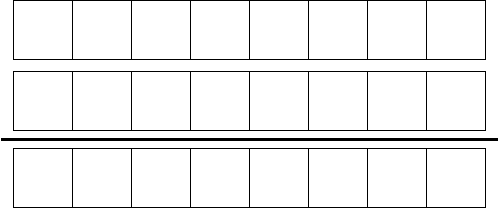
\includegraphics{representation_nombres_ordinateurs_files/figure-pdf/unnamed-chunk-11-1.pdf}

La valeur est donc donnée par:

\[
(-1)^{b_{31}}\times 2^{(b_{30}b_{29}\ldots b_{23})_2-127}\times (1,b_{22}b_{21}\ldots b_0)_2
\] ce qui donne \[
\text{valeur}=(-1)^{\text{signe}}\times 2^{(E-127)}\times \left( 1+ \sum_{i=1}^{23} b_{23-i} 2^{-i}\right)
\]

Dans l'exemple précédent, nous avons:

\begin{itemize}
\tightlist
\item
  signe = \(b_{31}\) = 0;
\item
  \((-1)^{\text{signe}}=(-1)^0=+1\in \{-1,+1\}\);
\item
  \(E=(b_{30}b_{29}\ldots b_{23})_2=\sum_{i=0}^7 b_{23+i}2^{+i}=124\in \{1,\ldots, (2^8-1)-1\}=\{1,\ldots, 254\}\);
\item
  \(2^{(E-127)}=2^{124-127}=2^{-3}\in \{2^{-126},\ldots, 2^{127}\}\);
\item
  \(1,b_{22}b_{21}\ldots b_0=1+\sum_{i=1}^{23} b_{23-i}2^{-i}=1+1\cdot 2^{-2}=1,25\in \{1,1+2^{-23},\ldots, 2-2^{-23}\} \subset [1;2-2^{-23}] \subset [1;2[\)
\end{itemize}

\hypertarget{lencodage-de-lexposant}{%
\subsubsection*{L'encodage de l'exposant}\label{lencodage-de-lexposant}}
\addcontentsline{toc}{subsubsection}{L'encodage de l'exposant}

L'exposant du format à virgule flottante à précision simple est encodé
de manière biaisée, avec un biais de 127 (\(2^{e-1}-1=2^{8-1}-1\)).

\begin{itemize}
\tightlist
\item
  E\textsubscript{min}=01\textsubscript{16}-7F\textsubscript{16}=-126
\item
  E\textsubscript{max}=FE\textsubscript{16}-7F\textsubscript{16}=127
\item
  Biais de l'exposant = 7F\textsubscript{16}=127
\end{itemize}

Pour obtenir l'exposant véritable, on doit soustraire 127 à l'exposant
stocké.

Les exposants 00\textsubscript{16} et FF\textsubscript{16} ont une
interprétation spéciale.

\begin{longtable}[]{@{}
  >{\raggedright\arraybackslash}p{(\columnwidth - 6\tabcolsep) * \real{0.1504}}
  >{\raggedright\arraybackslash}p{(\columnwidth - 6\tabcolsep) * \real{0.1203}}
  >{\raggedright\arraybackslash}p{(\columnwidth - 6\tabcolsep) * \real{0.1504}}
  >{\raggedright\arraybackslash}p{(\columnwidth - 6\tabcolsep) * \real{0.5789}}@{}}
\toprule\noalign{}
\begin{minipage}[b]{\linewidth}\raggedright
Exposant
\end{minipage} & \begin{minipage}[b]{\linewidth}\raggedright
Fraction = 0
\end{minipage} & \begin{minipage}[b]{\linewidth}\raggedright
Fraction \(\neq\) 0
\end{minipage} & \begin{minipage}[b]{\linewidth}\raggedright
Équation
\end{minipage} \\
\midrule\noalign{}
\endhead
\bottomrule\noalign{}
\endlastfoot
00\textsubscript{16} & \(\pm\) zéro & nombre dénormalisé &
\((-1)^{\text{signe}}\times 2^{-126}\times 0,\text{fraction}\) \\
01\textsubscript{16},\ldots,FE\textsubscript{16} & valeur normale &
valeur normale &
\((-1)^{\text{signe}}\times 2^{\text{exposant}-127}\times 1,\text{fraction}\) \\
FF\textsubscript{16} & \(\pm\) infini & NaN & \\
\end{longtable}

\hypertarget{cas-particuliers-dans-le-format-virgule-flottante-uxe0-pruxe9cision-simple}{%
\subsubsection*{Cas particuliers dans le format virgule flottante à
précision
simple}\label{cas-particuliers-dans-le-format-virgule-flottante-uxe0-pruxe9cision-simple}}
\addcontentsline{toc}{subsubsection}{Cas particuliers dans le format
virgule flottante à précision simple}

Pour les exemples suivants, trouvez la représentation sous forme binaire
et hexadécimale.

\begin{example}[]\protect\hypertarget{exm-plus-petit-nombre-denormalise}{}\label{exm-plus-petit-nombre-denormalise}

Trouvez le plus petit nombre dénormalisé positif.

\end{example}

\begin{example}[]\protect\hypertarget{exm-plus-grand-nombre-denormalise}{}\label{exm-plus-grand-nombre-denormalise}

Trouvez le plus grand nombre dénormalisé positif.

\end{example}

\begin{example}[]\protect\hypertarget{exm-plus-petit-nombre-normalise}{}\label{exm-plus-petit-nombre-normalise}

Trouvez le plus petit nombre normalisé positif.

\end{example}

\begin{example}[]\protect\hypertarget{exm-plus-grand-nombre-normalise}{}\label{exm-plus-grand-nombre-normalise}

Trouvez le plus grand nombre normalisé positif.

\end{example}

\begin{example}[]\protect\hypertarget{exm-plus-grand-nombre-plus-petit-un}{}\label{exm-plus-grand-nombre-plus-petit-un}

Trouvez le plus grand nombre plus petit que un.

\end{example}

\hypertarget{le-format-uxe0-virgule-flottante-uxe0-pruxe9cision-double}{%
\subsection{Le format à virgule flottante à précision
double}\label{le-format-uxe0-virgule-flottante-uxe0-pruxe9cision-double}}

\href{https://evanw.github.io/float-toy/}{Float Toy}

\href{https://introcs.cs.princeton.edu/java/91float/}{Princeton Float}

\href{https://hackingcpp.com/cpp/lang/fundamental_types.html}{Cheatsheets
for ieee 754 representation}

\href{https://www.wikiwand.com/fr/IEEE\%20754}{IEEE754 Wiki Wand}

\bookmarksetup{startatroot}

\hypertarget{logique}{%
\chapter{Logique}\label{logique}}

\hypertarget{logique-propositionnelle}{%
\section{Logique propositionnelle}\label{logique-propositionnelle}}

\begin{definition}[Proposition]\protect\hypertarget{def-proposition}{}\label{def-proposition}

Un énoncé qui est soit vrai, soit faux est appelé une
\textbf{proposition}. La \textbf{valeur de vérité} d'une proposition est
donc \textbf{VRAI} ou \textbf{FAUX}.

En \texttt{Python}, les valeurs de vérités sont données par
\texttt{True} (\textbf{VRAI}) et \texttt{False} (\textbf{FAUX}).

\end{definition}

Un énoncé qui n'est pas une proposition (comme un paradoxe, une phrase
impérative ou interrogative) sera qualifié d'innaceptable.

\begin{example}[]\protect\hypertarget{exm-propositions}{}\label{exm-propositions}

Les énoncés suivants sont des propositions:

\begin{itemize}
\tightlist
\item
  Les numéros de téléphones au Canada ont dix chiffres.
\item
  La lune est faite de fromage.
\item
  42 est la réponse à la question portant sur la \emph{vie, l'univers et
  tout ce qui existe}.
\item
  Chaque nombre pair plus grand que 2 peut être exprimé comme la somme
  de deux nombres premiers.
\item
  \(3+7=12\)
\end{itemize}

Les énoncés suivants ne sont \textbf{pas} des propositions:

\begin{itemize}
\tightlist
\item
  Voulez-vous du gâteau?
\item
  La somme de deux carrés.
\item
  \(1+3+5+7+\ldots +2n+1\).
\item
  Va dans ta chambre!
\item
  \(3+x=12\)
\end{itemize}

\end{example}

Nous utilisons une table de vérité pour montrer les valeurs de vérité de
propositions composées.

\hypertarget{la-nuxe9gation}{%
\subsection{La négation}\label{la-nuxe9gation}}

\begin{definition}[La
négation]\protect\hypertarget{def-negation}{}\label{def-negation}

Soit \(p\) une proposition. L'énoncé:

\begin{quote}
\emph{Il n'est pas vrai que \(p\).}
\end{quote}

est une autre proposition appelée \textbf{négation} de \(p\), qui est
représentée par \(\lnot p\). La proposition \(\lnot p\) se lit \emph{non
\(p\)}. La table de vérité de la négation est donnée ci-dessous.

\begin{longtable}[]{@{}cc@{}}
\toprule\noalign{}
\(p\) & \(\lnot p\) \\
\midrule\noalign{}
\endhead
\bottomrule\noalign{}
\endlastfoot
\(\phantom{V}\) & \(\phantom{V}\) \\
\(\phantom{V}\) & \(\phantom{V}\) \\
\end{longtable}

En \texttt{Python}, l'opérateur \texttt{not} permet de faire la négation
d'une valeur de vérité.

\hypertarget{negation-python}{}
\begin{Shaded}
\begin{Highlighting}[]
\KeywordTok{def}\NormalTok{ negation(p):}
    \ControlFlowTok{return} \KeywordTok{not}\NormalTok{ p}

\BuiltInTok{print}\NormalTok{(}\StringTok{"p    non\_p"}\NormalTok{)}
\ControlFlowTok{for}\NormalTok{ p }\KeywordTok{in}\NormalTok{ [}\VariableTok{True}\NormalTok{, }\VariableTok{False}\NormalTok{]:}
\NormalTok{    non\_p }\OperatorTok{=}\NormalTok{ negation(p)}
    \BuiltInTok{print}\NormalTok{(p, non\_p)}
\end{Highlighting}
\end{Shaded}

\begin{verbatim}
p    non_p
True False
False True
\end{verbatim}

\end{definition}

\hypertarget{la-conjonction}{%
\subsection{La conjonction}\label{la-conjonction}}

\begin{quote}
Je suis une roche \textbf{ET} je suis une île.
\end{quote}

\begin{definition}[La
conjonction]\protect\hypertarget{def-conjonction}{}\label{def-conjonction}

Soit \(p\) et \(q\) deux propositions. La proposition \emph{\(p\) et
\(q\)}, notée \(p\wedge q\), est vraie si à la fois \(p\) et \(q\) sont
vraies. Elle est fausse dans tous les autres cas. Cette proposition est
appelée la \textbf{conjonction} de \(p\) et de \(q\). La table de vérité
de la conjonction est donnée ci-dessous.

\begin{longtable}[]{@{}ccc@{}}
\toprule\noalign{}
\(p\) & \(q\) & \(p \wedge q\) \\
\midrule\noalign{}
\endhead
\bottomrule\noalign{}
\endlastfoot
\(\phantom{V}\) & \(\phantom{V}\) & \(\phantom{V}\) \\
\(\phantom{V}\) & \(\phantom{V}\) & \(\phantom{V}\) \\
\(\phantom{V}\) & \(\phantom{V}\) & \(\phantom{V}\) \\
\(\phantom{V}\) & \(\phantom{V}\) & \(\phantom{V}\) \\
\end{longtable}

En \texttt{Python}, l'opérateur \texttt{and} permet de faire la
conjonction de deux valeurs de vérité.

\hypertarget{conjonction-python}{}
\begin{Shaded}
\begin{Highlighting}[]
\KeywordTok{def}\NormalTok{ conjonction(p, q):}
    \ControlFlowTok{return}\NormalTok{ p }\KeywordTok{and}\NormalTok{ q}

\BuiltInTok{print}\NormalTok{(}\StringTok{"p    q    p\_et\_q"}\NormalTok{)}
\ControlFlowTok{for}\NormalTok{ p }\KeywordTok{in}\NormalTok{ [}\VariableTok{True}\NormalTok{, }\VariableTok{False}\NormalTok{]:}
    \ControlFlowTok{for}\NormalTok{ q }\KeywordTok{in}\NormalTok{ [}\VariableTok{True}\NormalTok{, }\VariableTok{False}\NormalTok{]:}
\NormalTok{        p\_et\_q }\OperatorTok{=}\NormalTok{ conjonction(p, q)}
        \BuiltInTok{print}\NormalTok{(p, q, p\_et\_q)}
\end{Highlighting}
\end{Shaded}

\begin{verbatim}
p    q    p_et_q
True True True
True False False
False True False
False False False
\end{verbatim}

\end{definition}

\hypertarget{la-disjonction}{%
\subsection{La disjonction}\label{la-disjonction}}

\begin{quote}
Elle a étudié très fort \textbf{OU} elle est extrêmement brillante.
\end{quote}

\begin{definition}[La
disjonction]\protect\hypertarget{def-disjonction}{}\label{def-disjonction}

Soit \(p\) et \(q\) deux propositions. La proposition \emph{\(p\) ou
\(q\)}, notée \(p\vee q\), est fausse si \(p\) et \(q\) sont fausses.
Elle est vraie dans tous les autres cas. Cette proposition est appelée
la \textbf{disjonction} de \(p\) et de \(q\). La table de vérité de la
disjonction est donnée ci-dessous.

\begin{longtable}[]{@{}ccc@{}}
\toprule\noalign{}
\(p\) & \(q\) & \(p \vee q\) \\
\midrule\noalign{}
\endhead
\bottomrule\noalign{}
\endlastfoot
\(\phantom{V}\) & \(\phantom{V}\) & \(\phantom{V}\) \\
\(\phantom{V}\) & \(\phantom{V}\) & \(\phantom{V}\) \\
\(\phantom{V}\) & \(\phantom{V}\) & \(\phantom{V}\) \\
\(\phantom{V}\) & \(\phantom{V}\) & \(\phantom{V}\) \\
\end{longtable}

En \texttt{Python}, l'opérateur \texttt{or} permet de faire la
disjonction de deux valeurs de vérité.

\hypertarget{disjonction-python}{}
\begin{Shaded}
\begin{Highlighting}[]
\KeywordTok{def}\NormalTok{ disjonction(p, q):}
    \ControlFlowTok{return}\NormalTok{ p }\KeywordTok{or}\NormalTok{ q}

\BuiltInTok{print}\NormalTok{(}\StringTok{"p    q    p\_ou\_q"}\NormalTok{)}
\ControlFlowTok{for}\NormalTok{ p }\KeywordTok{in}\NormalTok{ [}\VariableTok{True}\NormalTok{, }\VariableTok{False}\NormalTok{]:}
    \ControlFlowTok{for}\NormalTok{ q }\KeywordTok{in}\NormalTok{ [}\VariableTok{True}\NormalTok{, }\VariableTok{False}\NormalTok{]:}
\NormalTok{        p\_ou\_q }\OperatorTok{=}\NormalTok{ disjonction(p, q)}
        \BuiltInTok{print}\NormalTok{(p, q, p\_ou\_q)}
\end{Highlighting}
\end{Shaded}

\begin{verbatim}
p    q    p_ou_q
True True True
True False True
False True True
False False False
\end{verbatim}

\end{definition}

\hypertarget{la-disjonction-exclusive}{%
\subsection{La disjonction exclusive}\label{la-disjonction-exclusive}}

\begin{quote}
Prenez \textbf{SOIT} deux Advil \textbf{OU} deux Tylenols.
\end{quote}

\begin{definition}[La disjonction
exclusive]\protect\hypertarget{def-disjonction-exclusive}{}\label{def-disjonction-exclusive}

Soit \(p\) et \(q\) deux propositions. La proposition \emph{\(p\) ou
exclusif \(q\)}, notée \(p\oplus q\), est vraie si \(p\) et \(q\) ont
des valeurs de vérité \textbf{différentes}. Elle est fausse dans tous
les autres cas. Cette proposition est appelée la \textbf{disjonction
exclusive} de \(p\) et de \(q\). La table de vérité de la disjonction
exclusive est donnée ci-dessous.

\begin{longtable}[]{@{}ccc@{}}
\toprule\noalign{}
\(p\) & \(q\) & \(p \oplus q\) \\
\midrule\noalign{}
\endhead
\bottomrule\noalign{}
\endlastfoot
\(\phantom{V}\) & \(\phantom{V}\) & \(\phantom{V}\) \\
\(\phantom{V}\) & \(\phantom{V}\) & \(\phantom{V}\) \\
\(\phantom{V}\) & \(\phantom{V}\) & \(\phantom{V}\) \\
\(\phantom{V}\) & \(\phantom{V}\) & \(\phantom{V}\) \\
\end{longtable}

En \texttt{Python}, il n'existe pas d'opérateur logique pour effectuer
la disjonction exclusive. On peut par contre utiliser l'opérateur bit à
bit \texttt{\^{}} pour faire cette disjonction exclusive.

\end{definition}

\begin{example}[]\protect\hypertarget{exm-disjonction-exclusive-python}{}\label{exm-disjonction-exclusive-python}

Utilisez les opérateurs logiques vus précédemment pour construire la
table de vérité de la disjonction exclusive dans \texttt{Python}.

\hypertarget{disjonction-exclusive-python-todo}{}
\begin{Shaded}
\begin{Highlighting}[]
\KeywordTok{def}\NormalTok{ disjonction\_exclusive(p, q):}
    \ControlFlowTok{return} \CommentTok{\#REMPLACEZ MOI\#}

\BuiltInTok{print}\NormalTok{(}\StringTok{"p    q    p\_ou\_exclusif\_q"}\NormalTok{)}
\ControlFlowTok{for}\NormalTok{ p }\KeywordTok{in}\NormalTok{ [}\VariableTok{True}\NormalTok{, }\VariableTok{False}\NormalTok{]:}
    \ControlFlowTok{for}\NormalTok{ q }\KeywordTok{in}\NormalTok{ [}\VariableTok{True}\NormalTok{, }\VariableTok{False}\NormalTok{]:}
\NormalTok{        p\_ou\_exclusif\_q }\OperatorTok{=}\NormalTok{ disjonction\_exclusive(p, q)}
        \BuiltInTok{print}\NormalTok{(p, q, p\_ou\_exclusif\_q)}
\end{Highlighting}
\end{Shaded}

\hypertarget{disjonction-exclusive-python}{}
\begin{verbatim}
p    q    p_ou_exclusif_q
True True False
True False True
False True True
False False False
\end{verbatim}

\end{example}

\begin{tcolorbox}[enhanced jigsaw, colbacktitle=quarto-callout-important-color!10!white, toptitle=1mm, left=2mm, toprule=.15mm, opacityback=0, bottomrule=.15mm, breakable, coltitle=black, title=\textcolor{quarto-callout-important-color}{\faExclamation}\hspace{0.5em}{Important}, colframe=quarto-callout-important-color-frame, arc=.35mm, titlerule=0mm, rightrule=.15mm, opacitybacktitle=0.6, leftrule=.75mm, bottomtitle=1mm, colback=white]

La disjonction exclusive signifie l'un ou l'autre, mais pas les deux.

\end{tcolorbox}

\hypertarget{limplication}{%
\subsection{L'implication}\label{limplication}}

\begin{quote}
\textbf{SI} vous avez 100 à l'examen final, \textbf{ALORS} vous
obtiendrez A dans ce cours.
\end{quote}

\begin{definition}[L'implication]\protect\hypertarget{def-implication}{}\label{def-implication}

Soit \(p\) et \(q\) deux propositions. L'\textbf{implication}
\(p\rightarrow q\) est une proposition qui est fausse quand \(p\) est
vraie et que \(q\) est fausse, et qui est vraie dans tous les autres
cas. Dans une implication, \(p\) est appelée l'\textbf{hypothèse} (ou
l'\textbf{antécédent} ou la \textbf{prémisse}) et \(q\), la
\textbf{conclusion} (ou la \textbf{conséquence}). La table de vérité de
l'implication' est donnée ci-dessous.

\begin{longtable}[]{@{}ccc@{}}
\toprule\noalign{}
\(p\) & \(q\) & \(p \rightarrow q\) \\
\midrule\noalign{}
\endhead
\bottomrule\noalign{}
\endlastfoot
\(\phantom{V}\) & \(\phantom{V}\) & \(\phantom{V}\) \\
\(\phantom{V}\) & \(\phantom{V}\) & \(\phantom{V}\) \\
\(\phantom{V}\) & \(\phantom{V}\) & \(\phantom{V}\) \\
\(\phantom{V}\) & \(\phantom{V}\) & \(\phantom{V}\) \\
\end{longtable}

En \texttt{Python}, il n'existe pas d'opérateur logique pour effectuer
l'implication.

\end{definition}

\begin{example}[]\protect\hypertarget{exm-implication-python}{}\label{exm-implication-python}

Utilisez les opérateurs logiques vus précédemment pour construire la
table de vérité de l'implication dans \texttt{Python}.

\hypertarget{implication-python-todo}{}
\begin{Shaded}
\begin{Highlighting}[]
\KeywordTok{def}\NormalTok{ implication(p, q):}
    \ControlFlowTok{return} \CommentTok{\#REMPLACEZ MOI\#}

\BuiltInTok{print}\NormalTok{(}\StringTok{"p    q    p\_implique\_q"}\NormalTok{)}
\ControlFlowTok{for}\NormalTok{ p }\KeywordTok{in}\NormalTok{ [}\VariableTok{True}\NormalTok{, }\VariableTok{False}\NormalTok{]:}
    \ControlFlowTok{for}\NormalTok{ q }\KeywordTok{in}\NormalTok{ [}\VariableTok{True}\NormalTok{, }\VariableTok{False}\NormalTok{]:}
\NormalTok{        p\_implique\_q }\OperatorTok{=}\NormalTok{ implication(p, q)}
        \BuiltInTok{print}\NormalTok{(p, q, p\_implique\_q)}
\end{Highlighting}
\end{Shaded}

\hypertarget{implication-python}{}
\begin{verbatim}
p    q    p_implique_q
True True True
True False False
False True True
False False True
\end{verbatim}

\end{example}

\begin{tcolorbox}[enhanced jigsaw, colbacktitle=quarto-callout-important-color!10!white, toptitle=1mm, left=2mm, toprule=.15mm, opacityback=0, bottomrule=.15mm, breakable, coltitle=black, title=\textcolor{quarto-callout-important-color}{\faExclamation}\hspace{0.5em}{Important}, colframe=quarto-callout-important-color-frame, arc=.35mm, titlerule=0mm, rightrule=.15mm, opacitybacktitle=0.6, leftrule=.75mm, bottomtitle=1mm, colback=white]

Une implication peut être considérée comme un \textbf{contrat} qui
échoue seulement si les conditions du contrat sont respectées mais les
résultats ne sont pas remplis.

\end{tcolorbox}

Comme les implications apparaissent constamment en mathématiques, il
existe une vaste terminologie pour désigner \(p\rightarrow q\). Voici
les modes les plus courants:

\begin{itemize}
\tightlist
\item
  si \(p\) alors \(q\);
\item
  \(p\) implique \(q\);
\item
  \(p\) seulement si \(q\);
\item
  \(p\) est suffisant pour \(q\);
\item
  \(q\) si \(p\);
\item
  \(q\) chaque fois que \(p\);
\item
  \(q\) est nécessaire à \(p\).
\end{itemize}

\hypertarget{la-biconditionnelle}{%
\subsection{La biconditionnelle}\label{la-biconditionnelle}}

\begin{quote}
Il pleut dehors \textbf{SI ET SEULEMENT SI} c'est un jour nuageux.
\end{quote}

\begin{definition}[La
biconditionnelle]\protect\hypertarget{def-biconditionnelle}{}\label{def-biconditionnelle}

Soit \(p\) et \(q\) deux propositions. La \textbf{biconditionnelle}
\(p\leftrightarrow q\) est une proposition qui est vraie quand \(p\) et
\(q\) ont les mêmes valeurs de vérité et qui est fausse dans les autres
cas. La table de vérité de la biconditionnelle est donnée ci-dessous.

\begin{longtable}[]{@{}ccc@{}}
\toprule\noalign{}
\(p\) & \(q\) & \(p \leftrightarrow q\) \\
\midrule\noalign{}
\endhead
\bottomrule\noalign{}
\endlastfoot
\(\phantom{V}\) & \(\phantom{V}\) & \(\phantom{V}\) \\
\(\phantom{V}\) & \(\phantom{V}\) & \(\phantom{V}\) \\
\(\phantom{V}\) & \(\phantom{V}\) & \(\phantom{V}\) \\
\(\phantom{V}\) & \(\phantom{V}\) & \(\phantom{V}\) \\
\end{longtable}

En \texttt{Python}, il n'existe pas d'opérateur logique pour effectuer
la biconditionnelle.

\end{definition}

\begin{example}[]\protect\hypertarget{exm-biconditionnelle-python}{}\label{exm-biconditionnelle-python}

Utilisez les opérateurs logiques vus précédemment pour construire la
table de vérité de la biconditionnelle dans \texttt{Python}.

\hypertarget{biconditionnelle-python-todo}{}
\begin{Shaded}
\begin{Highlighting}[]
\KeywordTok{def}\NormalTok{ biconditionnelle(p, q):}
    \ControlFlowTok{return} \CommentTok{\#REMPLACEZ MOI\#}

\BuiltInTok{print}\NormalTok{(}\StringTok{"p    q    p\_biconditionnelle\_q"}\NormalTok{)}
\ControlFlowTok{for}\NormalTok{ p }\KeywordTok{in}\NormalTok{ [}\VariableTok{True}\NormalTok{, }\VariableTok{False}\NormalTok{]:}
    \ControlFlowTok{for}\NormalTok{ q }\KeywordTok{in}\NormalTok{ [}\VariableTok{True}\NormalTok{, }\VariableTok{False}\NormalTok{]:}
\NormalTok{        p\_biconditionnelle\_q }\OperatorTok{=}\NormalTok{ biconditionnelle(p, q)}
        \BuiltInTok{print}\NormalTok{(p, q, p\_biconditionnelle\_q)}
\end{Highlighting}
\end{Shaded}

\hypertarget{biconditionnelle-python}{}
\begin{verbatim}
p    q    p_biconditionnelle_q
True True True
True False False
False True False
False False True
\end{verbatim}

\end{example}

\begin{tcolorbox}[enhanced jigsaw, colbacktitle=quarto-callout-important-color!10!white, toptitle=1mm, left=2mm, toprule=.15mm, opacityback=0, bottomrule=.15mm, breakable, coltitle=black, title=\textcolor{quarto-callout-important-color}{\faExclamation}\hspace{0.5em}{Important}, colframe=quarto-callout-important-color-frame, arc=.35mm, titlerule=0mm, rightrule=.15mm, opacitybacktitle=0.6, leftrule=.75mm, bottomtitle=1mm, colback=white]

La biconditionnelle est vraie si les propositions ont la même valeur de
vérité et fausse autrement.

\end{tcolorbox}

Comme les biconditionnelles apparaissent constamment en mathématiques,
il existe une vaste terminologie pour désigner \(p\leftrightarrow q\).
Voici les modes les plus courants:

\begin{itemize}
\tightlist
\item
  \(p\) si et seulement si \(q\);
\item
  \(p\) est nécessaire et suffisante pour \(q\);
\item
  si \(p\) alors \(q\) et réciproquement.
\end{itemize}

\begin{definition}[Réciproque, contraposée et
inverse]\protect\hypertarget{def-reciproque-contraposee-inverse}{}\label{def-reciproque-contraposee-inverse}

~

\begin{itemize}
\tightlist
\item
  La \textbf{réciproque} de la proposition \(p\rightarrow q\) est la
  proposition \(q \rightarrow p\).
\item
  La \textbf{contraposée} de la proposition \(p\rightarrow q\) est la
  proposition \(\lnot q \rightarrow \lnot p\).
\item
  L'\textbf{inverse} de la proposition \(p\rightarrow q\) est la
  proposition \(\lnot p \rightarrow \lnot q\).
\end{itemize}

\end{definition}

\hypertarget{uxe9quivalences-propositionnelles}{%
\section{Équivalences
propositionnelles}\label{uxe9quivalences-propositionnelles}}

Une proposition composée est une proposition formée de plusieurs
connecteurs logiques.

\begin{definition}[Tautologie, contradiction et
contingence]\protect\hypertarget{def-tautologie-contradiction-contingence}{}\label{def-tautologie-contradiction-contingence}

Une proposition composée qui est toujours vraie, quelle que soit la
valeur de vérité des fonctions qui la compose est appelée une
\textbf{tautologie}. Une proposition composée qui est toujours fausse
est appelée une \textbf{contradiction}. Finalement, une proposition qui
n'est ni une tautologie ni une contradiction est appelée une
\textbf{contingence}.

\end{definition}

\begin{example}[]\protect\hypertarget{exm-tautologie-contradiction}{}\label{exm-tautologie-contradiction}

Remplissez la table de vérité suivante et dites si les propositions
composées sont des tautologies, des contradictions ou des contingences.

\begin{longtable}[]{@{}
  >{\centering\arraybackslash}p{(\columnwidth - 6\tabcolsep) * \real{0.2206}}
  >{\centering\arraybackslash}p{(\columnwidth - 6\tabcolsep) * \real{0.2206}}
  >{\centering\arraybackslash}p{(\columnwidth - 6\tabcolsep) * \real{0.2647}}
  >{\centering\arraybackslash}p{(\columnwidth - 6\tabcolsep) * \real{0.2941}}@{}}
\toprule\noalign{}
\begin{minipage}[b]{\linewidth}\centering
\(p\)
\end{minipage} & \begin{minipage}[b]{\linewidth}\centering
\(q\)
\end{minipage} & \begin{minipage}[b]{\linewidth}\centering
\(p \vee \lnot p\)
\end{minipage} & \begin{minipage}[b]{\linewidth}\centering
\(p \wedge \lnot p\)
\end{minipage} \\
\midrule\noalign{}
\endhead
\bottomrule\noalign{}
\endlastfoot
\(\phantom{V}\) & \(\phantom{V}\) & \(\phantom{V}\) & \(\phantom{V}\) \\
\(\phantom{V}\) & \(\phantom{V}\) & \(\phantom{V}\) & \(\phantom{V}\) \\
\end{longtable}

\end{example}

\begin{example}[]\protect\hypertarget{exm-proposition-compose}{}\label{exm-proposition-compose}

Le code ci-dessous révèle la table de vérité de la proposition composée
\((p \wedge q) \vee \lnot q\).

\hypertarget{prop-composee-1}{}
\begin{Shaded}
\begin{Highlighting}[]
\KeywordTok{def}\NormalTok{ conjonction(p, q):}
    \ControlFlowTok{return}\NormalTok{ p }\KeywordTok{and}\NormalTok{ q}

\KeywordTok{def}\NormalTok{ disjonction(p, q):}
    \ControlFlowTok{return}\NormalTok{ p }\KeywordTok{or}\NormalTok{ q}

\BuiltInTok{print}\NormalTok{(}\StringTok{"p    q    a"}\NormalTok{)}
\ControlFlowTok{for}\NormalTok{ p }\KeywordTok{in}\NormalTok{ [}\VariableTok{True}\NormalTok{, }\VariableTok{False}\NormalTok{]:}
    \ControlFlowTok{for}\NormalTok{ q }\KeywordTok{in}\NormalTok{ [}\VariableTok{True}\NormalTok{, }\VariableTok{False}\NormalTok{]:}
\NormalTok{        a }\OperatorTok{=}\NormalTok{ disjonction(conjonction(p, q), }\KeywordTok{not}\NormalTok{ q)}
        \BuiltInTok{print}\NormalTok{(p, q, a)}
\end{Highlighting}
\end{Shaded}

\begin{verbatim}
p    q    a
True True True
True False True
False True False
False False True
\end{verbatim}

De quelle manière pouvez-vous modifier le code précédent pour obtenir la
table de vérité de la proposition composée
\((p \vee \lnot q) \wedge \lnot p\)?

\end{example}

Lorsque vous créez votre table de vérité, il est crucial que vous soyiez
systématique pour vous assurer d'avoir toutes les valeurs de vérité
possibles pour chacune des propositions simples. Chaque proposition a
deux valeurs de vérité possibles, le nombre de lignes de la table
devrait être égal à \(2^n\), où \(n\) est le nombre de propositions.
Vous devriez également considérer de briser vos propositions complexes
en plus petites propositions.

\begin{example}[]\protect\hypertarget{exm-bloc-code}{}\label{exm-bloc-code}

L'extrait de code suivant fait intervenir les variables booléennes
\(p\), \(q\) et \(r\). Chacune de ces variables peut prendre les valeurs
\textbf{vrai} ou \textbf{faux}. Pour chaque bloc indiqué, donnez toutes
les valeurs possibles pour \(p\), \(q\) et \(r\) au moment où le bloc
est atteint.

\hypertarget{bloc-code-python}{}
\begin{Shaded}
\begin{Highlighting}[]
\ControlFlowTok{if}\NormalTok{ (p }\KeywordTok{and}\NormalTok{ q):}
    \ControlFlowTok{if}\NormalTok{ r:}
        \CommentTok{\#BLOC 1\#}
    \ControlFlowTok{else}\NormalTok{:}
        \CommentTok{\#BLOC 2\#}
\ControlFlowTok{else}\NormalTok{:}
    \CommentTok{\#BLOC 3\#}
\end{Highlighting}
\end{Shaded}

\begin{longtable}[]{@{}
  >{\centering\arraybackslash}p{(\columnwidth - 10\tabcolsep) * \real{0.1061}}
  >{\centering\arraybackslash}p{(\columnwidth - 10\tabcolsep) * \real{0.1061}}
  >{\centering\arraybackslash}p{(\columnwidth - 10\tabcolsep) * \real{0.1061}}
  >{\centering\arraybackslash}p{(\columnwidth - 10\tabcolsep) * \real{0.2273}}
  >{\centering\arraybackslash}p{(\columnwidth - 10\tabcolsep) * \real{0.2273}}
  >{\centering\arraybackslash}p{(\columnwidth - 10\tabcolsep) * \real{0.2273}}@{}}
\toprule\noalign{}
\begin{minipage}[b]{\linewidth}\centering
\(p\)
\end{minipage} & \begin{minipage}[b]{\linewidth}\centering
\(q\)
\end{minipage} & \begin{minipage}[b]{\linewidth}\centering
\(r\)
\end{minipage} & \begin{minipage}[b]{\linewidth}\centering
\(\phantom{V}\)
\end{minipage} & \begin{minipage}[b]{\linewidth}\centering
\(\phantom{V}\)
\end{minipage} & \begin{minipage}[b]{\linewidth}\centering
\(\phantom{V}\)
\end{minipage} \\
\midrule\noalign{}
\endhead
\bottomrule\noalign{}
\endlastfoot
\textbf{V} & \textbf{V} & \textbf{V} & & & \\
\textbf{V} & \textbf{V} & \textbf{F} & & & \\
\textbf{V} & \textbf{F} & \textbf{V} & & & \\
\textbf{V} & \textbf{F} & \textbf{F} & & & \\
\textbf{F} & \textbf{V} & \textbf{V} & & & \\
\textbf{F} & \textbf{V} & \textbf{F} & & & \\
\textbf{F} & \textbf{F} & \textbf{V} & & & \\
\textbf{F} & \textbf{F} & \textbf{F} & & & \\
\end{longtable}

\end{example}

\begin{definition}[Équivalences de
propositions]\protect\hypertarget{def-propositions-equivalentes}{}\label{def-propositions-equivalentes}

Les propositions \(p\) et \(q\) sont dites \textbf{logiquement
équivalentes} si la proposition \(p \leftrightarrow q\) est une
tautologie. Ainsi, deux propositions sont logiquement équivalentes si
elles ont la même table de vérité, c'est-à-dire la même valeur de vérité
dans tous les cas possibles.

La notation \(p\equiv q\) signifie que \(p\) et \(q\) sont équivalentes.

\end{definition}

\begin{example}[]\protect\hypertarget{exm-proposition-equivalentes-1}{}\label{exm-proposition-equivalentes-1}

Vérifiez l'équivalence suivante à l'aide d'une table de vérité. \[
p \rightarrow q \equiv \lnot p \vee q
\]

\begin{longtable}[]{@{}ccccc@{}}
\toprule\noalign{}
\(p\) & \(q\) & \(\phantom{V}\) & \(\phantom{V}\) & \(\phantom{V}\) \\
\midrule\noalign{}
\endhead
\bottomrule\noalign{}
\endlastfoot
\textbf{V} & \textbf{V} & & & \\
\textbf{V} & \textbf{F} & & & \\
\textbf{F} & \textbf{V} & & & \\
\textbf{F} & \textbf{F} & & & \\
\end{longtable}

\end{example}

\begin{example}[]\protect\hypertarget{exm-proposition-equivalentes-2}{}\label{exm-proposition-equivalentes-2}

Vérifiez l'équivalence suivante à l'aide d'une table de vérité. \[
\lnot (p \vee q) \equiv \lnot p \wedge \lnot q
\]

\begin{longtable}[]{@{}
  >{\centering\arraybackslash}p{(\columnwidth - 12\tabcolsep) * \real{0.0787}}
  >{\centering\arraybackslash}p{(\columnwidth - 12\tabcolsep) * \real{0.0787}}
  >{\centering\arraybackslash}p{(\columnwidth - 12\tabcolsep) * \real{0.1685}}
  >{\centering\arraybackslash}p{(\columnwidth - 12\tabcolsep) * \real{0.1685}}
  >{\centering\arraybackslash}p{(\columnwidth - 12\tabcolsep) * \real{0.1685}}
  >{\centering\arraybackslash}p{(\columnwidth - 12\tabcolsep) * \real{0.1685}}
  >{\centering\arraybackslash}p{(\columnwidth - 12\tabcolsep) * \real{0.1685}}@{}}
\toprule\noalign{}
\begin{minipage}[b]{\linewidth}\centering
\(p\)
\end{minipage} & \begin{minipage}[b]{\linewidth}\centering
\(q\)
\end{minipage} & \begin{minipage}[b]{\linewidth}\centering
\(\phantom{V}\)
\end{minipage} & \begin{minipage}[b]{\linewidth}\centering
\(\phantom{V}\)
\end{minipage} & \begin{minipage}[b]{\linewidth}\centering
\(\phantom{V}\)
\end{minipage} & \begin{minipage}[b]{\linewidth}\centering
\(\phantom{V}\)
\end{minipage} & \begin{minipage}[b]{\linewidth}\centering
\(\phantom{V}\)
\end{minipage} \\
\midrule\noalign{}
\endhead
\bottomrule\noalign{}
\endlastfoot
\textbf{V} & \textbf{V} & & & & & \\
\textbf{V} & \textbf{F} & & & & & \\
\textbf{F} & \textbf{V} & & & & & \\
\textbf{F} & \textbf{F} & & & & & \\
\end{longtable}

\end{example}

Pour gagner du temps, on note les équivalences fréquemment utilisées
dans une table et on leur donne un nom ou un numéro afin d'y faire
référence.

\hypertarget{tbl-equivalences-logiques}{}
\begin{longtable}[]{@{}
  >{\raggedright\arraybackslash}p{(\columnwidth - 4\tabcolsep) * \real{0.1620}}
  >{\raggedright\arraybackslash}p{(\columnwidth - 4\tabcolsep) * \real{0.4155}}
  >{\raggedright\arraybackslash}p{(\columnwidth - 4\tabcolsep) * \real{0.4225}}@{}}
\caption{\label{tbl-equivalences-logiques}Équivalences
logiques}\tabularnewline
\toprule\noalign{}
\begin{minipage}[b]{\linewidth}\raggedright
\textbf{Nom}
\end{minipage} & \begin{minipage}[b]{\linewidth}\raggedright
\textbf{Équivalence 1}
\end{minipage} & \begin{minipage}[b]{\linewidth}\raggedright
\textbf{Équivalence 2}
\end{minipage} \\
\midrule\noalign{}
\endfirsthead
\toprule\noalign{}
\begin{minipage}[b]{\linewidth}\raggedright
\textbf{Nom}
\end{minipage} & \begin{minipage}[b]{\linewidth}\raggedright
\textbf{Équivalence 1}
\end{minipage} & \begin{minipage}[b]{\linewidth}\raggedright
\textbf{Équivalence 2}
\end{minipage} \\
\midrule\noalign{}
\endhead
\bottomrule\noalign{}
\endlastfoot
\textbf{Identité} & \(p \wedge \mathbf{V} \equiv p\) &
\(p \vee \mathbf{F} \equiv p\) \\
\textbf{Domination} & \(p \vee \mathbf{V} \equiv \mathbf{V}\) &
\(p \wedge \mathbf{F} \equiv \mathbf{F}\) \\
\textbf{Idempotence} & \(p \vee p \equiv p\) & \(p\wedge p \equiv p\) \\
\textbf{Double négation} & \(\lnot (\lnot p) \equiv p\) & \\
\textbf{Commutativité} & \(p\wedge q \equiv q \wedge p\) &
\(p \vee q \equiv q \vee p\) \\
\textbf{Associativité} & \((p \vee q) \vee r \equiv p \vee (q \vee r)\)
& \((p \wedge q) \wedge r \equiv p \wedge (q \wedge r)\) \\
\textbf{Distributivité} &
\(p \vee (q \wedge r) \equiv (p \vee q) \wedge (p \vee r)\) &
\(p\wedge (q \vee r) \equiv (p \wedge q) \vee (p \wedge r)\) \\
\textbf{Lois de De Morgan} &
\(\lnot (p \wedge q) \equiv \lnot p \vee \lnot q\) &
\(\lnot (p \vee q) \equiv \lnot p \wedge \lnot q\) \\
\textbf{Absorption} & \(p \vee (p \wedge q) \equiv p\) &
\(p \wedge (p \vee q) \equiv p\) \\
\textbf{Négation} & \(p \vee \lnot p \equiv \mathbf{V}\) &
\(p \wedge \lnot p \equiv \mathbf{F}\) \\
\end{longtable}

\hypertarget{tbl-equivalences-logiques-implications}{}
\begin{longtable}[]{@{}
  >{\raggedright\arraybackslash}p{(\columnwidth - 2\tabcolsep) * \real{0.1333}}
  >{\raggedright\arraybackslash}p{(\columnwidth - 2\tabcolsep) * \real{0.8667}}@{}}
\caption{\label{tbl-equivalences-logiques-implications}Équivalences
logiques (implications)}\tabularnewline
\toprule\noalign{}
\begin{minipage}[b]{\linewidth}\raggedright
\textbf{Numéro}
\end{minipage} & \begin{minipage}[b]{\linewidth}\raggedright
\textbf{Implication}
\end{minipage} \\
\midrule\noalign{}
\endfirsthead
\toprule\noalign{}
\begin{minipage}[b]{\linewidth}\raggedright
\textbf{Numéro}
\end{minipage} & \begin{minipage}[b]{\linewidth}\raggedright
\textbf{Implication}
\end{minipage} \\
\midrule\noalign{}
\endhead
\bottomrule\noalign{}
\endlastfoot
\textbf{1} & \(p \rightarrow q \equiv \lnot p \vee q\) \\
\textbf{2} & \(p \rightarrow q \equiv \lnot q \rightarrow \lnot p\) \\
\textbf{3} & \(p \vee q \equiv \lnot p \rightarrow q\) \\
\textbf{4} & \(p \wedge q \equiv \lnot(p \rightarrow \lnot q)\) \\
\textbf{5} & \(\lnot(p \rightarrow q) \equiv p \wedge \lnot q\) \\
\textbf{6} &
\((p \rightarrow q)\wedge (p\rightarrow r) \equiv p \rightarrow (q \wedge r)\) \\
\textbf{7} &
\((p \rightarrow r) \wedge (q \rightarrow r) \equiv (p \vee q) \rightarrow r\) \\
\textbf{8} &
\((p\rightarrow q) \vee (p \rightarrow r) \equiv p \rightarrow (q \vee r)\) \\
\textbf{9} &
\((p \rightarrow r) \vee (q \rightarrow r) \equiv (p \wedge q) \rightarrow r\) \\
\end{longtable}

\hypertarget{tbl-equivalences-logiques-biconditionnelles}{}
\begin{longtable}[]{@{}
  >{\raggedright\arraybackslash}p{(\columnwidth - 2\tabcolsep) * \real{0.1224}}
  >{\raggedright\arraybackslash}p{(\columnwidth - 2\tabcolsep) * \real{0.8776}}@{}}
\caption{\label{tbl-equivalences-logiques-biconditionnelles}Équivalences
logiques (biconditionnelles)}\tabularnewline
\toprule\noalign{}
\begin{minipage}[b]{\linewidth}\raggedright
\textbf{Numéro}
\end{minipage} & \begin{minipage}[b]{\linewidth}\raggedright
\textbf{Biconditionnelle}
\end{minipage} \\
\midrule\noalign{}
\endfirsthead
\toprule\noalign{}
\begin{minipage}[b]{\linewidth}\raggedright
\textbf{Numéro}
\end{minipage} & \begin{minipage}[b]{\linewidth}\raggedright
\textbf{Biconditionnelle}
\end{minipage} \\
\midrule\noalign{}
\endhead
\bottomrule\noalign{}
\endlastfoot
\textbf{1} &
\(p \leftrightarrow q \equiv (p\rightarrow q) \wedge (q \rightarrow q)\) \\
\textbf{2} &
\(p \leftrightarrow q \equiv \lnot p \leftrightarrow \lnot q\) \\
\textbf{3} &
\(p \leftrightarrow q \equiv (p \wedge q) \vee (\lnot p \wedge \lnot q)\) \\
\textbf{4} &
\(p \leftrightarrow q \equiv \lnot(p \wedge \lnot q) \wedge \lnot(\lnot p \wedge q )\) \\
\textbf{5} &
\(\lnot(p \leftrightarrow q) \equiv p \leftrightarrow \lnot q\) \\
\end{longtable}

\begin{example}[]\protect\hypertarget{exm-proposition-tautologie-deux-manieres}{}\label{exm-proposition-tautologie-deux-manieres}

Vérifiez que la proposition \[
\lnot (p \rightarrow q) \rightarrow \lnot q
\] est une tautologie

\begin{enumerate}
\def\labelenumi{\alph{enumi}.}
\item
  à l'aide d'une table de vérité;

  \begin{longtable}[]{@{}
    >{\centering\arraybackslash}p{(\columnwidth - 12\tabcolsep) * \real{0.0787}}
    >{\centering\arraybackslash}p{(\columnwidth - 12\tabcolsep) * \real{0.0787}}
    >{\centering\arraybackslash}p{(\columnwidth - 12\tabcolsep) * \real{0.1685}}
    >{\centering\arraybackslash}p{(\columnwidth - 12\tabcolsep) * \real{0.1685}}
    >{\centering\arraybackslash}p{(\columnwidth - 12\tabcolsep) * \real{0.1685}}
    >{\centering\arraybackslash}p{(\columnwidth - 12\tabcolsep) * \real{0.1685}}
    >{\centering\arraybackslash}p{(\columnwidth - 12\tabcolsep) * \real{0.1685}}@{}}
  \toprule\noalign{}
  \begin{minipage}[b]{\linewidth}\centering
  \(p\)
  \end{minipage} & \begin{minipage}[b]{\linewidth}\centering
  \(q\)
  \end{minipage} & \begin{minipage}[b]{\linewidth}\centering
  \(\phantom{V}\)
  \end{minipage} & \begin{minipage}[b]{\linewidth}\centering
  \(\phantom{V}\)
  \end{minipage} & \begin{minipage}[b]{\linewidth}\centering
  \(\phantom{V}\)
  \end{minipage} & \begin{minipage}[b]{\linewidth}\centering
  \(\phantom{V}\)
  \end{minipage} & \begin{minipage}[b]{\linewidth}\centering
  \(\phantom{V}\)
  \end{minipage} \\
  \midrule\noalign{}
  \endhead
  \bottomrule\noalign{}
  \endlastfoot
  \textbf{V} & \textbf{V} & & & & & \\
  \textbf{V} & \textbf{F} & & & & & \\
  \textbf{F} & \textbf{V} & & & & & \\
  \textbf{F} & \textbf{F} & & & & & \\
  \end{longtable}
\item
  sans l'aide d'une table de vérité, en utilisant les tableaux
  d'équivalences.
\end{enumerate}

\end{example}

\begin{tcolorbox}[enhanced jigsaw, colbacktitle=quarto-callout-important-color!10!white, toptitle=1mm, left=2mm, toprule=.15mm, opacityback=0, bottomrule=.15mm, breakable, coltitle=black, title=\textcolor{quarto-callout-important-color}{\faExclamation}\hspace{0.5em}{Propositions équivalentes ou non?}, colframe=quarto-callout-important-color-frame, arc=.35mm, titlerule=0mm, rightrule=.15mm, opacitybacktitle=0.6, leftrule=.75mm, bottomtitle=1mm, colback=white]

Pour démontrer que les propositions \textbf{ne sont pas} équivalentes,
il suffit de fournir des valeurs de \(p\), \(q\) et \(r\) pour
lesquelles elles diffèrent. Pour démontrer que les propositions sont
équivalentes, on peut procéder de l'une des trois façons suivantes.

\begin{enumerate}
\def\labelenumi{\arabic{enumi}.}
\tightlist
\item
  Fournir leur table de vérité.
\item
  Utiliser la Table~\ref{tbl-equivalences-logiques}, la
  Table~\ref{tbl-equivalences-logiques-implications} ou la
  Table~\ref{tbl-equivalences-logiques-biconditionnelles}.
\item
  Formuler une explication en mots qui montre que les deux propositions
  sont vraies, ou encore que les deux sont fausses, exactement pour les
  mêmes combinaisons de valeur de vérité des variables
  propositionnelles.
\end{enumerate}

\end{tcolorbox}

\hypertarget{pruxe9dicats-et-quantificateurs}{%
\section{Prédicats et
quantificateurs}\label{pruxe9dicats-et-quantificateurs}}

Un énoncé contenant une ou plusieurs variables tel que \[
x<10 \quad \text{ou} \quad x+2=7-y
\] n'est pas une proposition pusique, tant que la valeur de \(x\) ou
\(y\) n'est pas connue, on ne peut dire s'il est vrai ou faux.

\begin{definition}[Terminologie]\protect\hypertarget{def-sujet-predicat}{}\label{def-sujet-predicat}

Dans l'énoncé ``\(x<10\)'', \(x\) est le \textbf{sujet}, et ``est
inférieur à 10'' est le \textbf{prédicat}. Notons \(P(x)\) l'énoncé
\(x<10\). On dit que \(P\) est une \textbf{fonction propositionnelle}.

\end{definition}

Une fonction propositionnelle \(P(x)\) prend la valeur vrai ou faux
quand \(x\) est précisé. Par exemple:

\begin{itemize}
\tightlist
\item
  \(P(8)\) est une proposition vraie. On écrira parfois \(P(8)\) est
  vrai (au masculin, en sous-entendant l'énoncé est vrai, ou même
  \(P(8)\equiv \mathbf{V}\)).
\item
  \(P(13)\) est une proposition fausse.
\item
  \(P(\text{Marc-André})\) n'est pas une proposition, car
  \emph{Marc-André} n'est pas une valeur possible pour la variable
  \(x\).
\end{itemize}

L'ensemble des valeurs possibles pour la variable \(x\) est appelé
\textbf{univers du discours}, ou \textbf{domaine} de la fonction \(P\).

\begin{definition}[Quantificateurs]\protect\hypertarget{def-quantificateurs}{}\label{def-quantificateurs}

\[
\forall:\ \text{quantificateur universel} \qquad \exists:\ \text{quantificateur existentiel}
\]

\begin{description}
\tightlist
\item[\(\forall\ x\ P(x)\):]
signifie ``Pour toutes les valeurs de \(x\) dans l'univers du discours,
\(P(x)\)''. Ou encore ``Quel que soit \(x\) (dans l'univers du
discours), \(P(x)\)''.
\item[\(\exists\ x\ P(x)\):]
signifie ``Il existe un élément de \(x\) dans l'univers du discours tel
que \(P(x)\)''. Ou encore ``Il y a au moins un \(x\) (dans l'univers du
discours) tel que \(P(x)\)''. Ou encore ``Pour un certain \(x\) (dans
l'univers du discours), \(P(x)\)''.
\end{description}

\textbf{Notation}. Certains auteurs mettent une virgule avant la
fonction propositionnelle, surtout quand celle-ci est composée. Par
exemple: \(\forall\ x,\ (P_1(x)\rightarrow P_2(x) \vee P_3(x))\). Par
ailleurs, si l'ensemble \(U\) n'a pas déjà été identifié, on peut
préciser que la variable \(x\) prendra des valeurs dans l'ensemble \(U\)
ainsi: \(\exists\ x\in U,\ P(x)\).

\end{definition}

Lorsque l'univers du discours est un ensemble fini
\(\{x_1,x_2,\ldots, x_n\}\), on a les équivalences logiques suivantes:

\begin{align*}
\forall\ x\ P(x) &\equiv P(x_1)\wedge P(x_2) \wedge \cdots \wedge P(x_n) \\
\exists\ x\ P(x) &\equiv P(x_1)\vee P(x_2) \vee \cdots \vee P(x_n)
\end{align*}

La quantification universelle \(\forall\ x\ P(x)\) est vraie quand
\(P(x)\) est vraie pour toutes les valeurs de \(x\) dans l'univers du
discours \(U\). Elle est donc fausse s'il existe un \(x\) de \(U\) pour
lequel \(P(x)\) est fausse. Un tel élément est appelé un
\textbf{contre-exemple} de \(\forall\ x\ P(x)\).

La quantification existentielle \(\exists\ x\ P(x)\) est vraie s'il
existe au moins une valeur \(x\) dans l'univers du discours telle que
\(P(x)\) est vraie. Elle est fausse si \(P(x)\) est fausse pour toutes
les valeurs possibles de \(x\).

Ainsi, pour prouver un énoncé de la forme \(\forall\ x\ P(x)\) est vrai,
fournir un exemple de \(x\) tel que \(P(x)\) est vrai ne suffit pas. Il
faut montrer que la proposition \(P(x)\) est vraie pour toutes les
valeurs de \(x\), ce qui peut s'avérer particulièrement
\textbf{difficile lorsque \(U\) est un ensemble infini}. Il en va de
même losqu'on veut prouver qu'un énoncé de la forme \(\exists\ x\ P(x)\)
est faux.

\hypertarget{tbl-prouver-enonce-univers-infini}{}
\begin{longtable}[]{@{}
  >{\raggedright\arraybackslash}p{(\columnwidth - 4\tabcolsep) * \real{0.0948}}
  >{\raggedright\arraybackslash}p{(\columnwidth - 4\tabcolsep) * \real{0.4502}}
  >{\raggedright\arraybackslash}p{(\columnwidth - 4\tabcolsep) * \real{0.4550}}@{}}
\caption{\label{tbl-prouver-enonce-univers-infini}Comment prouver qu'un
énoncé quantifié est vrai ou faux quand l'univers du discours \(U\) est
infini.}\tabularnewline
\toprule\noalign{}
\begin{minipage}[b]{\linewidth}\raggedright
Pour prouver que
\end{minipage} & \begin{minipage}[b]{\linewidth}\raggedright
est \textbf{vrai}
\end{minipage} & \begin{minipage}[b]{\linewidth}\raggedright
est \textbf{faux}
\end{minipage} \\
\midrule\noalign{}
\endfirsthead
\toprule\noalign{}
\begin{minipage}[b]{\linewidth}\raggedright
Pour prouver que
\end{minipage} & \begin{minipage}[b]{\linewidth}\raggedright
est \textbf{vrai}
\end{minipage} & \begin{minipage}[b]{\linewidth}\raggedright
est \textbf{faux}
\end{minipage} \\
\midrule\noalign{}
\endhead
\bottomrule\noalign{}
\endlastfoot
\(\exists\ x\ P(x)\) & il suffit de fournir \textbf{un exemple}: un
\(x\) de \(U\) tel que \(P(x)\) est vrai. & il faut fournir un argument
général pour montrer que \(P(x)\) est faux quel que soit \(x\) de
\(U\). \\
\(\forall\ x\ P(x)\) & il faut fournir un argument général pour montrer
que \$P(x) est vrai quel que soit \(x\) de \(U\). & il suffit de fournir
un \textbf{contre-exemple}: un \(x\) de \(U\) tel que \(P(x)\) est
faux. \\
\end{longtable}

\begin{example}[]\protect\hypertarget{exm-univers-discours-nombres-reels}{}\label{exm-univers-discours-nombres-reels}

Si l'univers du discours est l'ensemble des nombres réels et
\begin{align*}
&P(x)\ \text{désigne}\ x\geq 0 \\
&Q(x)\ \text{désigne}\ x\ \text{est un nombre premier} \\
&R(x)\ \text{désigne}\ 3^x+4^x=5^x \\
&S(x)\ \text{désigne}\ x\geq 100
\end{align*} dites si chacun des énoncés suivants est une proposition
vraie, une proposition fausse ou n'est pas une proposition. Donnez un
exemple ou un contre-exemple le cas échéant. Dans le cas contraire,
indiquez qu'un argument général est requis.

\begin{enumerate}
\def\labelenumi{\alph{enumi}.}
\tightlist
\item
  \(\forall\ x\ P(x)\)
\item
  \(\forall\ x\ \lnot P(x)\)
\item
  \(\forall\ x\ P(x^2)\)
\item
  \(\exists\ x\ P(x)\)
\item
  \(\exists\ x\ \lnot P(x)\)
\item
  \(\exists\ x\ Q(x)\)
\item
  \(\exists\ x\ Q(x^2)\)
\item
  \(\forall\ x\ R(x)\)
\item
  \(P(x)\)
\item
  \(\forall\ x\ (S(x)\rightarrow P(x))\)
\item
  \((\forall\ x\ P(x)) \rightarrow (\forall\ x\ S(x))\)
\item
  \(\forall\ x\ S(x+100)\)
\item
  \(\forall\ x\ S(x^2+100)\)
\end{enumerate}

\end{example}

\begin{theorem}[Lois de De Morgan pour les
quantificateurs]\protect\hypertarget{thm-de-morgan-quantificateurs}{}\label{thm-de-morgan-quantificateurs}

\[
\lnot \exists\ x\ P(x) \equiv \forall\ x\ \lnot P(x) \qquad \lnot \forall\ x\ P(x) \equiv \exists\ x\ \lnot P(x)
\]

\end{theorem}

\begin{example}[]\protect\hypertarget{exm-univers-etudiants-stjean-repertoire}{}\label{exm-univers-etudiants-stjean-repertoire}

Si l'univers du discours est l'ensemble des étudiants du programme
Sciences Informatique et Mathématique (ScIM) et \(M(x)\) désigne
l'énoncé \emph{l'étudiant \(x\) peut modifier les fichiers du répertoire
\(U\)}, traduisez clairement les propositions suivantes à l'aide des
quantificateurs.

\begin{enumerate}
\def\labelenumi{\alph{enumi}.}
\tightlist
\item
  Tous les étudiants de ScIM peuvent modifier les fichiers du répertoire
  \(U\).
\item
  Il est faux que tous les étudiants de ScIM peuvent modifier les
  fichiers du répertoire \(U\).
\item
  Au moins un étudiant de ScIM peut modifier les fichiers du répertoire
  \(U\).
\item
  Il est faux qu'au moins un étudiant de ScIM peut modifier les fichiers
  du répertoire \(U\).
\item
  Aucun étudiant de ScIM ne peut modifier les fichiers du répertoire
  \(U\).
\item
  Au moins un étudiant de ScIM ne peut pas modifier les fichiers du
  répertoire \(U\).
\end{enumerate}

De plus, déterminez les propositions ci-dessus qui sont équivalentes.

\end{example}

\begin{example}[]\protect\hypertarget{exm-univers-billes-rouges-bleues}{}\label{exm-univers-billes-rouges-bleues}

Si l'univers du discours est l'ensemble des billes contenues dans un
bol, et si

\begin{itemize}
\tightlist
\item
  \(G(x)\) désigne \emph{la bille \(x\) est grosse}
\item
  \(J(x)\) désigne \emph{la bille \(x\) est jaune}
\item
  \(R(x)\) désigne \emph{la bille \(x\) est rouge}
\item
  \(B(x)\) désigne \emph{la bille \(x\) est bleue}
\end{itemize}

traduisez clairement les propositions suivantes en prenant soin de bien
formuler les phrases.

\begin{enumerate}
\def\labelenumi{\alph{enumi}.}
\tightlist
\item
  \(\forall\ x\ (R(x) \vee J(x))\)
\item
  \((\forall\ x\ R(x)) \vee (\forall\ x\ J(x))\)
\item
  Les propositions a. et b. sont-elles équivalentes?
\item
  \(\exists\ x\ B(x)\)
\item
  \(\lnot(\exists\ x\ B(x))\)
\item
  Utilisez le quantificateur universel \(\forall\) pour écrire une
  proposition équivalente à la précédente.
\item
  \(\lnot(\forall\ x\ R(x))\)
\item
  Utilisez le quantificateur existentiel \(\exists\) pour écrire une
  proposition équivalente à la précédente.
\item
  \(\forall\ x\ (G(x) \rightarrow B(x))\)
\item
  \(\exists\ x\ (G(x) \wedge B(x))\)
\item
  \((\exists\ x\ G(x)) \wedge (\exists\ x\ B(x))\)
\item
  Les deux propositions précédentes sont-elles équivalentes?
\item
  Les deux propositions suivantes sont-elles équivalentes? \[
  (\exists\ x\ R(x)) \vee (\exists\ x\ J(x)) \qquad \text{et} \qquad \exists\ x\ (R(x) \vee J(x))
  \]
\item
  Les deux propositions suivantes sont-elles équivalentes? \[
  (\forall\ x\ R(x)) \wedge (\forall\ x\ G(x)) \qquad \text{et} \qquad \forall\ x\ (R(x) \wedge G(x))
  \]
\end{enumerate}

\end{example}

\hypertarget{opuxe9rations-bit-uxe0-bit}{%
\section{Opérations bit à bit}\label{opuxe9rations-bit-uxe0-bit}}

\hypertarget{probluxe8mes-de-logique}{%
\section{Problèmes de logique}\label{probluxe8mes-de-logique}}

Les problèmes suivants se déroulent sur une île imaginaire où tous les
habitants sont soit des \textbf{chevaliers}, qui disent toujours la
vérité, soit des \textbf{fripons}, qui mentent toujours. Ces énigmes
implique un visiteur qui rencontre un petit groupe d'habitants de l'île.
La plupart du temps, le but du visiteur est de \emph{déduire} les types
des habitants à partir de leurs énoncés.

Voici un exemple type de problème possible.

\begin{tcolorbox}[enhanced jigsaw, bottomrule=.15mm, breakable, colback=white, left=2mm, rightrule=.15mm, toprule=.15mm, arc=.35mm, opacityback=0, leftrule=.75mm]

\textbf{Déduisez!}\vspace{2mm}

En vous promenant sur l'île, vous rencontrez trois habitants gardant un
pont. Pour passer, vous devez déduire le type de chaque habitant. Chaque
individu dit un seul énoncé:

\begin{itemize}
\tightlist
\item
  Individu A: Si je suis un fripon, alors il y a exactement deux
  chevaliers ici.
\item
  Individu B: L'individu A ment.
\item
  Individu C: Soit nous sommes tous des fripons ou alors au moins l'un
  d'entre nous est un chevalier.
\end{itemize}

Quels sont les types des trois individus?

\end{tcolorbox}

\hypertarget{stratuxe9gies}{%
\subsection*{Stratégies}\label{stratuxe9gies}}
\addcontentsline{toc}{subsection}{Stratégies}

Voici quelques stratégies que vous pouvez utiliser pour résoudre ce
genre de problème:

\begin{itemize}
\tightlist
\item
  Commencez en supposant qu'un individu est d'un certain type. Soyez
  stratégique avec votre supposition, tentez de résoudre un énoncé
  \textbf{ET}.

  \begin{itemize}
  \tightlist
  \item
    Si un individu dit \textbf{ET}, supposez qu'il est un chevalier;
  \item
    Si un individu dit \textbf{OU}, supposez qu'il est un fripon;
  \item
    Si un individu dit \textbf{SI/ALORS}, supposez qu'il est un fripon;
  \item
    Si un individu dit \textbf{SI ET SEULEMENT SI}, attendez de
    connaître la valeur de vérité de leur énoncé avant de faire une
    supposition.
  \end{itemize}
\item
  Lorsqu'un individu est un chevalier, vous pouvez continuer leur
  énoncé.
\item
  Lorsqu'un individu est un fripon, vous pouvez continuer la négation de
  leur énoncé.

  \begin{itemize}
  \tightlist
  \item
    Partie 1 \textbf{ET} Partie 2 \(\rightarrow\) \textbf{NON} Partie 1
    \textbf{OU} \textbf{NON} Partie 2
  \item
    Partie 1 \textbf{OU} Partie 2 \(\rightarrow\) \textbf{NON} Partie 1
    \textbf{ET} \textbf{NON} Partie 2
  \item
    \textbf{SI} Partie 1, alors Partie 2 \(\rightarrow\) Partie 1
    \textbf{ET} \textbf{NON} Partie 2
  \end{itemize}
\item
  Soyez prudents avec les \emph{si et seulement si}

  \begin{itemize}
  \tightlist
  \item
    Lorsqu'un \emph{si et seulement si} est \texttt{VRAI}, alors les
    deux parties ont la \textbf{même} valeur de vérité.
  \item
    Lorsqu'un \emph{si et seulement si} est \texttt{FAUX}, alors les
    deux parties ont des valeurs de vérités \textbf{différentes}.
  \end{itemize}
\item
  Lorsque vous avez prouvé l'identité d'un individu, vous pouvez
  utiliser cette information partout dans le reste de l'énigme.
\item
  Si vous avez suffisament d'information pour confirmer que l'énoncé
  d'un individu est \texttt{VRAI}, alors ils doivent être un chevalier.
\item
  Si vous avez suffisament d'information pour confirmer que l'énoncé
  d'un individu est \texttt{FAUX}, alors ils doivent être un fripon.
\end{itemize}

\hypertarget{trois-uxe9noncuxe9s-diffuxe9rents}{%
\subsection{Trois énoncés
différents}\label{trois-uxe9noncuxe9s-diffuxe9rents}}

Nous pouvons, dans la plupart des problèmes, regrouper les énoncés des
habitants de l'île en trois formes distinctes.

\hypertarget{accusations-et-affirmations}{%
\subsubsection{Accusations et
affirmations}\label{accusations-et-affirmations}}

Dans une accusation, un habitant \emph{A} dit par exemple \emph{B est un
fripon} ou un énoncé équivalent comme \emph{B ment toujours}. Dans une
affirmation, l'habitant \emph{A} dit par exemple \emph{B est un
chevalier} ou alors \emph{B dit toujours la vérité}.

\begin{example}[]\protect\hypertarget{exm-accusation-different-types}{}\label{exm-accusation-different-types}

Que pouvez-vous conclure si \emph{A} et \emph{B} sont reliés par une
\textbf{accusation}?

\end{example}

\begin{example}[]\protect\hypertarget{exm-accusation-different-types}{}\label{exm-accusation-different-types}

Que pouvez-vous conclure si \emph{A} et \emph{B} sont reliés par une
\textbf{affirmation}?

\end{example}

\hypertarget{conjonctions-de-fripons}{%
\subsubsection{Conjonctions de fripons}\label{conjonctions-de-fripons}}

Un exemple de conjonction de fripons est lorsque \emph{A} dit que
\emph{B est un chevalier ou je suis un fripon}, ou alors \emph{C est un
fripon et je suis un fripon}

\begin{example}[]\protect\hypertarget{exm-conjonction-de-fripons-ou}{}\label{exm-conjonction-de-fripons-ou}

Que pouvez-vous conclure si \emph{A} et \emph{B} sont reliés par
\textbf{ou je suis un fripon}?

\end{example}

\begin{example}[]\protect\hypertarget{exm-conjonction-de-fripons-et}{}\label{exm-conjonction-de-fripons-et}

Que pouvez-vous conclure si \emph{A} et \emph{B} sont reliés par
\textbf{et je suis un fripon}?

\end{example}

\hypertarget{uxe9noncuxe9s-de-diffuxe9rences-ou-de-similarituxe9s}{%
\subsubsection{Énoncés de différences ou de
similarités}\label{uxe9noncuxe9s-de-diffuxe9rences-ou-de-similarituxe9s}}

Parfois un habitant \emph{A} dira \emph{B est de mon type} ou peut-être
\emph{C n'est pas de mon type}.

\begin{example}[]\protect\hypertarget{exm-similarite-fripons}{}\label{exm-similarite-fripons}

Que pouvez-vous conclure si \emph{A} dit que \emph{B est de son type}?

\end{example}

\begin{example}[]\protect\hypertarget{exm-difference-fripons}{}\label{exm-difference-fripons}

Que pouvez-vous conclure si \emph{A} dit que \emph{C n'est pas de son
type}?

\end{example}

Il est intéressant de comparer ces énoncés avec ceux d'accusations et
d'affirmations. Ces deux types d'énoncés sont réciproques en quelque
sorte. Lorsqu'un habitant dit directement de quel type est un autre
habitant (dans une accusation ou une affirmation), tout ce qu'on apprend
c'est que la source et la cible sont similaires ou différents, sans
apprendre leur type. Par contre, lorsqu'un habitant dit un énoncé par
rapport aux similitudes ou aux différences, nous apprenons exactement de
quel type la cible est, sans apprendre si elle est similaire ou
différente de la source.

\begin{example}[]\protect\hypertarget{exm-chevaliers-et-fripons-1}{}\label{exm-chevaliers-et-fripons-1}

Vous rencontrez trois habitants de l'île.

\begin{itemize}
\tightlist
\item
  A dit: B ne ment jamais.
\item
  A dit: C est un chevalier ou je suis un fripon.
\end{itemize}

\end{example}

\begin{example}[]\protect\hypertarget{exm-chevaliers-et-fripons-2}{}\label{exm-chevaliers-et-fripons-2}

Vous rencontrez trois habitants de l'île.

\begin{itemize}
\tightlist
\item
  A dit: B ment toujours.
\item
  B dit: A n'est pas de mon type.
\end{itemize}

\end{example}

\bookmarksetup{startatroot}

\hypertarget{thuxe9orie-des-ensembles}{%
\chapter{Théorie des ensembles}\label{thuxe9orie-des-ensembles}}

\hypertarget{notions-de-base-sur-les-ensembles}{%
\section{Notions de base sur les
ensembles}\label{notions-de-base-sur-les-ensembles}}

\begin{definition}[Ensemble,
élément]\protect\hypertarget{def-ensemble-element}{}\label{def-ensemble-element}

Un \textbf{ensemble} est un collection non ordonnée d'objets. Les objets
sont appelés \textbf{éléments} de l'ensemble et on dit qu'ils
appartiennent à l'ensemble.

Notation : \(x\in F\) signifie que \(x\) est un élément de l'ensemble
\(F\). On dit aussi que \(x\) appartient à l'ensemble \(F\).

\end{definition}

\begin{definition}[Ensemble fini ou infini,
cardinalité]\protect\hypertarget{def-ensemble-fini-infini-cardinalite}{}\label{def-ensemble-fini-infini-cardinalite}

Soit \(A\) un ensemble composé de \(n\) éléments distincts. On dit que
\(A\) est un \textbf{ensemble fini} de \textbf{cardinalité} \(n\) et on
note \(|A|=n\). Un ensemble est dit \textbf{infini} s'il n'est pas fini.

\end{definition}

\begin{example}[]\protect\hypertarget{exm-ensemble-simple}{}\label{exm-ensemble-simple}

Soit l'ensemble \(F=\set{2,\pi,7}\). Utilisez les symboles introduits
pour traduire les énoncés suivants: l'ensemble \(F\) contient 3
éléments, \(\pi\) appartient à \(F\), 5 n'appartient pas à \(F\).

\end{example}

On peut décrire un ensemble \textbf{en extension} (on énumère ses
éléments que l'on place entre accolades) \[
A=\set{5,7,9,11} \qquad B=\set{1,8,27,64}
\] ou en \textbf{compréhension}, comme ceci: \[
A=\set{x\in\mathbb{N}\mid (x\ \text{est impair}) \wedge (5\leq x \leq 11)} \qquad
B=\set{x\in\mathbb{N}\mid (x \leq 64) \wedge (\exists\ y\in \mathbb{N},\ y^3=x)}
\]

Pour créer un ensemble dans \texttt{Python}, nous allons utiliser une
paire d'accolades \texttt{\{} \texttt{\}} et placer les différents
éléments de notre ensemble entre ces accolades en les séparant avec une
virgule. De plus, nous pouvons vérifier si un élément appartient à
l'ensemble en utilisant la commande \texttt{in}.

\hypertarget{ensemble-accolades}{}
\begin{Shaded}
\begin{Highlighting}[]
\NormalTok{A}\OperatorTok{=}\NormalTok{\{}\OperatorTok{{-}}\DecValTok{2}\NormalTok{,}\DecValTok{0}\NormalTok{,}\DecValTok{1}\NormalTok{,}\DecValTok{4}\NormalTok{\}}
\BuiltInTok{print}\NormalTok{(A, }\DecValTok{1} \KeywordTok{in}\NormalTok{ A, }\DecValTok{5} \KeywordTok{in}\NormalTok{ A)}
\end{Highlighting}
\end{Shaded}

\begin{verbatim}
{0, 1, 4, -2} True False
\end{verbatim}

Pour calculer la cardinalité d'un ensemble dans \texttt{Python}, vous
utilisez la fonction \texttt{len()}. En \texttt{Python}, il faut être
prudent si on souhaite utiliser l'ensemble vide, \(\emptyset\). Si vous
utilisez \texttt{\{\}} pour décrire l'ensemble vide, \texttt{Python} va
plutôt l'interpréter comme un \emph{dictionnaire} vide. Vous devez
plutôt utiliser la fonction \texttt{set()}.

\hypertarget{cardinalite-python}{}
\begin{Shaded}
\begin{Highlighting}[]
\NormalTok{A }\OperatorTok{=}\NormalTok{ \{}\DecValTok{2}\NormalTok{,}\DecValTok{3}\NormalTok{,}\DecValTok{5}\NormalTok{,}\DecValTok{8}\NormalTok{\}}
\NormalTok{B }\OperatorTok{=} \BuiltInTok{set}\NormalTok{()}
\NormalTok{C }\OperatorTok{=}\NormalTok{ \{}\DecValTok{0}\NormalTok{\}}
\BuiltInTok{print}\NormalTok{(}\BuiltInTok{len}\NormalTok{(A), }\BuiltInTok{len}\NormalTok{(B), }\BuiltInTok{len}\NormalTok{(C))}
\end{Highlighting}
\end{Shaded}

\begin{verbatim}
4 0 1
\end{verbatim}

\hypertarget{ensembles-de-nombres-mathbbn-mathbbz-mathbbq-mathbbr}{%
\section{\texorpdfstring{Ensembles de nombres \(\mathbb{N}\),
\(\mathbb{Z}\), \(\mathbb{Q}\),
\(\mathbb{R}\)}{Ensembles de nombres \textbackslash mathbb\{N\}, \textbackslash mathbb\{Z\}, \textbackslash mathbb\{Q\}, \textbackslash mathbb\{R\}}}\label{ensembles-de-nombres-mathbbn-mathbbz-mathbbq-mathbbr}}

Nous détaillerons dans la Table~\ref{tbl-ensembles-nombres-usuels}, les
ensembles de nombres les plus communs.

\hypertarget{tbl-ensembles-nombres-usuels}{}
\begin{longtable}[]{@{}
  >{\raggedright\arraybackslash}p{(\columnwidth - 2\tabcolsep) * \real{0.5695}}
  >{\raggedright\arraybackslash}p{(\columnwidth - 2\tabcolsep) * \real{0.4305}}@{}}
\caption{\label{tbl-ensembles-nombres-usuels}Ensembles de nombres
usuels.}\tabularnewline
\toprule\noalign{}
\begin{minipage}[b]{\linewidth}\raggedright
\textbf{Ensemble}
\end{minipage} & \begin{minipage}[b]{\linewidth}\raggedright
\textbf{Description}
\end{minipage} \\
\midrule\noalign{}
\endfirsthead
\toprule\noalign{}
\begin{minipage}[b]{\linewidth}\raggedright
\textbf{Ensemble}
\end{minipage} & \begin{minipage}[b]{\linewidth}\raggedright
\textbf{Description}
\end{minipage} \\
\midrule\noalign{}
\endhead
\bottomrule\noalign{}
\endlastfoot
\(\emptyset = \set{\phantom{1}}\) & Ensemble vide (ne contient aucun
élément \(\mid\emptyset\mid=0\)) \\
\(\mathbb{N}=\set{0,1,2,3,\ldots}\) & Ensemble des nombres naturels \\
\(\mathbb{N^*}=\set{1,2,3,\ldots}\) & Ensemble des nombres naturels
strictement positifs \\
\(\mathbb{Z}=\set{\ldots,-2,-1,0,1,2,\ldots}\) & Ensemble des nombres
entiers \\
\(\mathbb{Z^*}=\set{\ldots,-2,-1,1,2,\ldots}\) & Ensemble des entiers
non nuls \\
\(\mathbb{Q}=\set{\frac{p}{q}\mid p\in\mathbb{Z},q\in\mathbb{Z}\ \text{et}\ q\neq 0}\)
& Ensemble des nombres rationnels \\
\(\mathbb{R}\) & Ensemble des nombres réels \\
\(\mathbb{R^+}=\set{x\in\mathbb{R}\mid x\geq 0}\) & Ensemble des nombres
réels positifs \\
\(\mathbb{C}=\set{a+bi\mid a\in \mathbb{R}\ \text{et}\ b\in\mathbb{R}}\)
avec \(i^2=-1\) & Ensemble des nombres complexes \\
\end{longtable}

\begin{example}[]\protect\hypertarget{exm-ensembles-creation-par-comprehension}{}\label{exm-ensembles-creation-par-comprehension}

Établissez un lien entre les ensembles décrits par compréhension aux
parties a. à f.~avec le même ensemble décrit par extension aux parties 1
à 6.

\begin{enumerate}
\def\labelenumi{\alph{enumi}.}
\tightlist
\item
  \(\set{x\in\mathbb{Z}\mid x^2=1}\)
\item
  \(\set{x\in\mathbb{Z}\mid x^3=1}\)
\item
  \(\set{x\in\mathbb{Z}\mid |x|\leq 2}\)
\item
  \(\set{x\in\mathbb{Z}\mid x^2 \leq 4}\)
\item
  \(\set{x\in\mathbb{Z}\mid x<|x|}\)
\item
  \(\set{x\in\mathbb{Z}\mid (x+1)^2=x^2+2x+1}\)
\end{enumerate}

\begin{enumerate}
\def\labelenumi{\arabic{enumi}.}
\tightlist
\item
  \(\set{-1,0,1}\)
\item
  \(\set{\ldots,-3,-2,-1,0,1,2,3,\ldots}\)
\item
  \(\set{1}\)
\item
  \(\set{\ldots,-3,-2,-1}\)
\item
  \(\set{-1,1}\)
\item
  \(\set{-2,-1,0,1,2}\)
\end{enumerate}

\end{example}

\begin{tcolorbox}[enhanced jigsaw, colbacktitle=quarto-callout-note-color!10!white, toptitle=1mm, left=2mm, toprule=.15mm, opacityback=0, bottomrule=.15mm, breakable, coltitle=black, title=\textcolor{quarto-callout-note-color}{\faInfo}\hspace{0.5em}{Note}, colframe=quarto-callout-note-color-frame, arc=.35mm, titlerule=0mm, rightrule=.15mm, opacitybacktitle=0.6, leftrule=.75mm, bottomtitle=1mm, colback=white]

Lorsqu'il y a trop d'éléments dans un ensemble pour être en mesure de
tous les écrire, nous utilisons souvent les trois-points (\(\ldots\))
lorsque la suite d'éléments est claire. Par exemple, nous avons: \[
\mathbb{Z}=\set{\ldots,-3,-2,-1,0,1,2,3,\ldots}
\]

\end{tcolorbox}

En \texttt{Python}, si vous avez un ensemble décrit par compréhension,
il est particulièrement facile de le créer avec une
\texttt{compréhension\ de\ liste}. L'idée est simple: simplifier le code
pour le rendre plus lisible et donc plus rapide à écrire et plus simple
à maintenir. La syntaxe est la suivante:

\begin{verbatim}
new_list = [function(item) for item in list if condition(item)]
new_list = {function(item) for item in list if condition(item)}
\end{verbatim}

Par exemple, si vous voulez créer l'ensemble
\(\set{x^3\mid 0\leq x < 10}\), nous pouvons le faire en \texttt{Python}
de la manière suivante:

\hypertarget{comprehension-de-liste}{}
\begin{Shaded}
\begin{Highlighting}[]
\NormalTok{ensemble }\OperatorTok{=}\NormalTok{ \{x}\OperatorTok{**}\DecValTok{3} \ControlFlowTok{for}\NormalTok{ x }\KeywordTok{in} \BuiltInTok{range}\NormalTok{(}\DecValTok{10}\NormalTok{)\}}
\NormalTok{liste }\OperatorTok{=}\NormalTok{ [x}\OperatorTok{**}\DecValTok{3} \ControlFlowTok{for}\NormalTok{ x }\KeywordTok{in} \BuiltInTok{range}\NormalTok{(}\DecValTok{10}\NormalTok{)]}
\BuiltInTok{print}\NormalTok{(ensemble, liste)}
\end{Highlighting}
\end{Shaded}

\begin{verbatim}
{0, 1, 64, 512, 8, 343, 216, 729, 27, 125} [0, 1, 8, 27, 64, 125, 216, 343, 512, 729]
\end{verbatim}

\begin{tcolorbox}[enhanced jigsaw, colbacktitle=quarto-callout-note-color!10!white, toptitle=1mm, left=2mm, toprule=.15mm, opacityback=0, bottomrule=.15mm, breakable, coltitle=black, title=\textcolor{quarto-callout-note-color}{\faInfo}\hspace{0.5em}{Note}, colframe=quarto-callout-note-color-frame, arc=.35mm, titlerule=0mm, rightrule=.15mm, opacitybacktitle=0.6, leftrule=.75mm, bottomtitle=1mm, colback=white]

Remarquez que dans l'ensemble, les éléments ne sont pas ordonnés, tandis
qu'ils le sont dans la liste.

\end{tcolorbox}

\begin{definition}[Égalité
d'ensembles]\protect\hypertarget{def-egalite-ensembles}{}\label{def-egalite-ensembles}

Deux ensembles sont dits égaux si et seulement s'ils contiennent
exactement les mêmes éléments. \[
A=B \leftrightarrow \forall\ x\ (x\in A \leftrightarrow x\in B)
\]

\end{definition}

\begin{example}[]\protect\hypertarget{exm-ensembles-egaux-oui-non}{}\label{exm-ensembles-egaux-oui-non}

Les ensembles suivants sont-ils égaux? \begin{align*}
\set{1,3,5} &\stackrel{?}{=} \set{3,5,1} \\
\set{1,3,5} &\stackrel{?}{=} \set{\set{1},\set{3},\set{5}}
\end{align*}

\end{example}

\begin{definition}[Sous-ensemble]\protect\hypertarget{def-sous-ensemble}{}\label{def-sous-ensemble}

L'ensemble \(A\) est \textbf{sous-ensemble} de l'ensemble \(B\) si et
seulement si tous les éléments de \(A\) sont aussi des éléments de
\(B\): \[
A \subseteq B \leftrightarrow \forall\ x\ (x\in A \rightarrow x\in B)
\] L'ensemble \(A\) est \textbf{sous-ensemble strict (ou propre)} de
l'ensemble \(B\) si et seulement si tous les éléments de \(A\) sont
aussi des éléments de \(B\) et \(A\) n'est pas égal à \(B\): \[
A \subset B \leftrightarrow A\subseteq B \wedge\ A\neq B
\]

\end{definition}

\begin{example}[]\protect\hypertarget{exm-sous-ensembles-verification}{}\label{exm-sous-ensembles-verification}

Convainquez-vous des affirmations suivantes. \begin{align*}
\set{1,2} &\subseteq \set{1,2,3,4,5} \\
\set{1,2} &\subset \set{1,2,3,4,5} \\
\set{2k\mid k\in\mathbb{N}} &= \set{0,2,4,6,\ldots}\subset\mathbb{N}
\end{align*}

\end{example}

\hypertarget{tbl-notation-theorie-ensembles}{}
\begin{longtable}[]{@{}
  >{\raggedright\arraybackslash}p{(\columnwidth - 2\tabcolsep) * \real{0.0927}}
  >{\raggedright\arraybackslash}p{(\columnwidth - 2\tabcolsep) * \real{0.9073}}@{}}
\caption{\label{tbl-notation-theorie-ensembles}Notation de la théorie
des ensembles.}\tabularnewline
\toprule\noalign{}
\begin{minipage}[b]{\linewidth}\raggedright
\textbf{Notation}
\end{minipage} & \begin{minipage}[b]{\linewidth}\raggedright
\textbf{Description}
\end{minipage} \\
\midrule\noalign{}
\endfirsthead
\toprule\noalign{}
\begin{minipage}[b]{\linewidth}\raggedright
\textbf{Notation}
\end{minipage} & \begin{minipage}[b]{\linewidth}\raggedright
\textbf{Description}
\end{minipage} \\
\midrule\noalign{}
\endhead
\bottomrule\noalign{}
\endlastfoot
\(\in\) & \(2\in\set{1,2,3}\) indique que 2 est \textbf{un élément de}
l'ensemble \(\set{1,2,3}\). \\
\(\not\in\) & \(4\not\in\set{1,2,3}\) indique que 4 \textbf{n'est pas un
élément de} l'ensemble \(\set{1,2,3}\). \\
\(\subseteq\) & \(A\subseteq B\) indique que \(A\) est un
\textbf{sous-ensemble} de \(B\): chaque élément de \(A\) est aussi un
élément de \(B\). \\
\(\subset\) & \(A\subset B\) indique que \(A\) est un
\textbf{sous-ensemble propre} de \(B\): chaque élément de \(A\) est
aussi un élément de \(B\), mais \(A\neq B\). \\
\end{longtable}

\begin{theorem}[]\protect\hypertarget{thm-sous-ensemble-vide}{}\label{thm-sous-ensemble-vide}

Pour tout ensemble \(A\), on a :

\begin{enumerate}
\def\labelenumi{\arabic{enumi}.}
\tightlist
\item
  \(\emptyset\subseteq A\)
\item
  \(A\subseteq A\)
\end{enumerate}

\end{theorem}

\begin{theorem}[]\protect\hypertarget{thm-sous-ensemble-egalite-ensemble}{}\label{thm-sous-ensemble-egalite-ensemble}

\(A=B\) si et seulement si \(A\subseteq B\) et \(B\subseteq A\).

\end{theorem}

En \texttt{Python}, nous pouvons utiliser la fonction \texttt{issubset}
pour vérifier qu'un ensemble est sous-ensemble d'un autre.

\hypertarget{sous-ensemble-verification}{}
\begin{Shaded}
\begin{Highlighting}[]
\NormalTok{A }\OperatorTok{=}\NormalTok{ \{}\DecValTok{2}\NormalTok{,}\DecValTok{4}\NormalTok{,}\DecValTok{6}\NormalTok{,}\DecValTok{8}\NormalTok{,}\DecValTok{10}\NormalTok{,}\DecValTok{12}\NormalTok{\}}
\NormalTok{B }\OperatorTok{=}\NormalTok{ \{}\DecValTok{4}\NormalTok{,}\DecValTok{8}\NormalTok{,}\DecValTok{12}\NormalTok{\}}
\BuiltInTok{print}\NormalTok{(A.issubset(B), B.issubset(A))}
\end{Highlighting}
\end{Shaded}

\begin{verbatim}
False True
\end{verbatim}

\hypertarget{produit-cartuxe9sien}{%
\section{Produit cartésien}\label{produit-cartuxe9sien}}

\begin{definition}[Produit
cartésien]\protect\hypertarget{def-produit-cartesien}{}\label{def-produit-cartesien}

Le \textbf{produit cartésien} des ennsembles \(A\) et \(B\), noté
\(A\times B\), est L'ensemble de tous les couples (paires ordonnées)
dont le premier élément appartient à \(A\) et le second, à \(B\): \[
A\times B = \set{(a,b)\mid\ a\in A\ \text{et}\ b\in B}
\] On généralise cette définition au produit cartésien de \(n\)
ensembles: \[
A_1 \times A_2 \times \ldots \times A_n = \set{(a_1,a_2,\ldots,a_n)\mid\ a_1\in A_1,\ldots, a_n\in A_n}
\]

\end{definition}

\begin{example}[]\protect\hypertarget{exm-ensembles-extension-produit-cartesien}{}\label{exm-ensembles-extension-produit-cartesien}

Décrivez en extension les produits cartésiens \(A\times B\) et
\(B\times A\), où \(A=\set{0,1,2}\) et \(B=\set{a,c}\).

\end{example}

\begin{definition}[Relation]\protect\hypertarget{def-relation}{}\label{def-relation}

Une \textbf{relation} entre les ensembles \(A\) et \(B\) est un
sous-ensemble du produit cartésien \(A\times B\).

\end{definition}

\begin{example}[]\protect\hypertarget{exm-relation-entre-A-et-B}{}\label{exm-relation-entre-A-et-B}

Soit \$A=\set{0,1,2} et \$B=\set{a,c}. L'ensemble \[
R=\set{(0,a),(1,c),(2,a)}\subseteq A\times B
\] est une relation de \(A\) dans \(B\).

\end{example}

\begin{definition}[]\protect\hypertarget{def-ensemble-des-parties}{}\label{def-ensemble-des-parties}

L'\textbf{ensmeble des parties} de \(A\), noté \(\mathcal{P}(A)\), est
l'ensemble de tous les sous-ensembles de \(A\). \[
B\in \mathcal{P}(A) \leftrightarrow B \subseteq A
\]

\end{definition}

\begin{example}[]\protect\hypertarget{exm-ensemble-des-parties-de-A-3-elements}{}\label{exm-ensemble-des-parties-de-A-3-elements}

Décrivez \(\mathcal{P}(A)\), l'ensemble des parties de \(A\), où
\(A=\set{0,1,2}\).

\begin{longtable}[]{@{}
  >{\raggedright\arraybackslash}p{(\columnwidth - 4\tabcolsep) * \real{0.1059}}
  >{\raggedright\arraybackslash}p{(\columnwidth - 4\tabcolsep) * \real{0.5412}}
  >{\raggedright\arraybackslash}p{(\columnwidth - 4\tabcolsep) * \real{0.3529}}@{}}
\toprule\noalign{}
\begin{minipage}[b]{\linewidth}\raggedright
\textbf{\(k\)}
\end{minipage} & \begin{minipage}[b]{\linewidth}\raggedright
\textbf{Sous-ensembles de \(A\) ayant \(k\) éléments}
\end{minipage} & \begin{minipage}[b]{\linewidth}\raggedright
\textbf{Nombre de sous-ensembles}
\end{minipage} \\
\midrule\noalign{}
\endhead
\bottomrule\noalign{}
\endlastfoot
0 & \(\emptyset\) & 1 \\
1 & \(\set{0}\), \(\set{1}\), \(\set{2}\) & 3 \\
2 & \(\set{0,1}\), \(\set{0,2}\), \(\set{1,2}\) & 3 \\
3 & \(\set{0,1,2}\) & 1 \\
\end{longtable}

\end{example}

\begin{example}[]\protect\hypertarget{exm-ensemble-des-parties-de-A-4-elements}{}\label{exm-ensemble-des-parties-de-A-4-elements}

Décrivez \(\mathcal{P}(A)\), l'ensemble des parties de \(A\), où
\(A=\set{0,1,2,3}\).

\begin{longtable}[]{@{}
  >{\raggedright\arraybackslash}p{(\columnwidth - 4\tabcolsep) * \real{0.1059}}
  >{\raggedright\arraybackslash}p{(\columnwidth - 4\tabcolsep) * \real{0.5412}}
  >{\raggedright\arraybackslash}p{(\columnwidth - 4\tabcolsep) * \real{0.3529}}@{}}
\toprule\noalign{}
\begin{minipage}[b]{\linewidth}\raggedright
\textbf{\(k\)}
\end{minipage} & \begin{minipage}[b]{\linewidth}\raggedright
\textbf{Sous-ensembles de \(A\) ayant \(k\) éléments}
\end{minipage} & \begin{minipage}[b]{\linewidth}\raggedright
\textbf{Nombre de sous-ensembles}
\end{minipage} \\
\midrule\noalign{}
\endhead
\bottomrule\noalign{}
\endlastfoot
0 & & \\
1 & & \\
2 & & \\
3 & & \\
4 & & \\
\end{longtable}

\end{example}

\hypertarget{opuxe9rations-sur-les-ensembles-cap-cup-oplus--}{%
\section{\texorpdfstring{Opérations sur les ensembles \(\cap\),
\(\cup\), \(\oplus\),
\(-\)}{Opérations sur les ensembles \textbackslash cap, \textbackslash cup, \textbackslash oplus, -}}\label{opuxe9rations-sur-les-ensembles-cap-cup-oplus--}}

Soit \(U\) l'ensemble universel et \(A\) et \(B\) des sous-ensembles de
\(U\). Les opérations suivantes génèrent des sous-ensembles de \(U\).

\hypertarget{tbl-operations-ensembles}{}
\begin{longtable}[]{@{}
  >{\raggedright\arraybackslash}p{(\columnwidth - 2\tabcolsep) * \real{0.3068}}
  >{\raggedright\arraybackslash}p{(\columnwidth - 2\tabcolsep) * \real{0.6932}}@{}}
\caption{\label{tbl-operations-ensembles}Les diverses opérations sur les
ensembles.}\tabularnewline
\toprule\noalign{}
\begin{minipage}[b]{\linewidth}\raggedright
\textbf{Opération}
\end{minipage} & \begin{minipage}[b]{\linewidth}\raggedright
\textbf{Forme mathématique}
\end{minipage} \\
\midrule\noalign{}
\endfirsthead
\toprule\noalign{}
\begin{minipage}[b]{\linewidth}\raggedright
\textbf{Opération}
\end{minipage} & \begin{minipage}[b]{\linewidth}\raggedright
\textbf{Forme mathématique}
\end{minipage} \\
\midrule\noalign{}
\endhead
\bottomrule\noalign{}
\endlastfoot
\textbf{Union} & \(\set{x\in U\mid\ x\in A\ \vee\ x\in B}\) \\
\textbf{Intersection} & \(\set{x\in U\mid\ x\in A\ \wedge\ x\in B}\) \\
\textbf{Différence} &
\(\set{x\in U\mid\ x\in A\ \wedge\ x\not\in B}=A\setminus B\) \\
\textbf{Différence symétrique} &
\(\set{x\in U\mid\ x\in A\ \oplus\ x\in B}\) \\
\textbf{Complément} & \(\set{x\in U\mid\ x\not\in A}=U-A\) \\
\end{longtable}

\begin{figure}

\begin{minipage}[t]{0.50\linewidth}

{\centering 

\raisebox{-\height}{

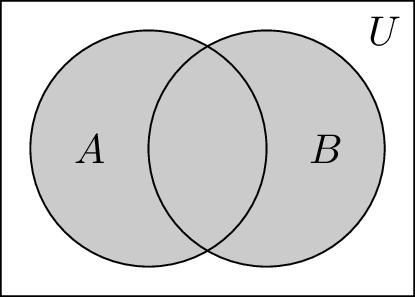
\includegraphics{tikz/union.png}

}

\caption{Union}

}

\end{minipage}%
%
\begin{minipage}[t]{0.50\linewidth}

{\centering 

\raisebox{-\height}{

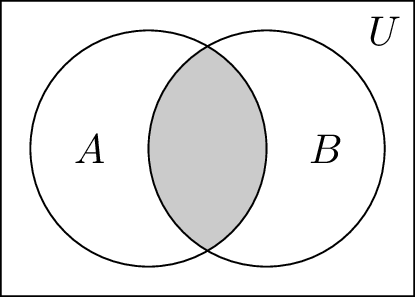
\includegraphics{tikz/intersection.png}

}

\caption{Intersection}

}

\end{minipage}%
\newline
\begin{minipage}[t]{0.50\linewidth}

{\centering 

\raisebox{-\height}{

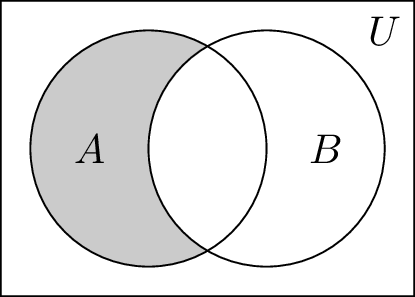
\includegraphics{tikz/difference.png}

}

\caption{Différence}

}

\end{minipage}%
%
\begin{minipage}[t]{0.50\linewidth}

{\centering 

\raisebox{-\height}{

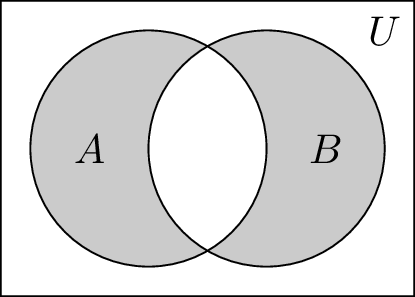
\includegraphics{tikz/difference_symetrique.png}

}

\caption{Différence symétrique}

}

\end{minipage}%
\newline
\begin{minipage}[t]{0.50\linewidth}

{\centering 

\raisebox{-\height}{

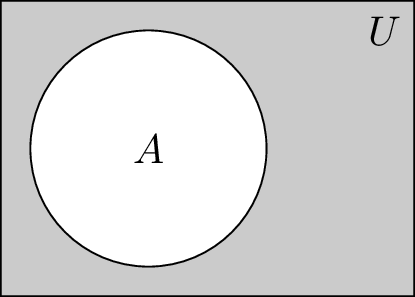
\includegraphics{tikz/complement.png}

}

\caption{Complément}

}

\end{minipage}%

\end{figure}

Vous pouvez effectuer ces opérations dans \texttt{Python} à l'aide des
commandes suivantes:

\hypertarget{tbl-operations-ensembles-python}{}
\begin{longtable}[]{@{}ll@{}}
\caption{\label{tbl-operations-ensembles-python}Les opérations sur les
ensembles dans \texttt{Python}.}\tabularnewline
\toprule\noalign{}
\textbf{Opération} & \textbf{Commande} \texttt{Python} \\
\midrule\noalign{}
\endfirsthead
\toprule\noalign{}
\textbf{Opération} & \textbf{Commande} \texttt{Python} \\
\midrule\noalign{}
\endhead
\bottomrule\noalign{}
\endlastfoot
\textbf{Union} & \texttt{union} \\
\textbf{Intersection} & \texttt{intersection} \\
\textbf{Différence} & \texttt{difference} \\
\end{longtable}

\hypertarget{union-python}{}
\begin{Shaded}
\begin{Highlighting}[]
\NormalTok{A }\OperatorTok{=}\NormalTok{ \{}\OperatorTok{{-}}\DecValTok{3}\NormalTok{,}\OperatorTok{{-}}\DecValTok{1}\NormalTok{,}\DecValTok{2}\NormalTok{,}\DecValTok{5}\NormalTok{\}}
\NormalTok{B }\OperatorTok{=}\NormalTok{ \{}\OperatorTok{{-}}\DecValTok{1}\NormalTok{, }\DecValTok{0}\NormalTok{, }\DecValTok{2}\NormalTok{\}}
\BuiltInTok{print}\NormalTok{(A.union(B))}
\end{Highlighting}
\end{Shaded}

\begin{verbatim}
{0, 2, 5, -3, -1}
\end{verbatim}

\hypertarget{intersection-python}{}
\begin{Shaded}
\begin{Highlighting}[]
\NormalTok{A }\OperatorTok{=}\NormalTok{ \{}\OperatorTok{{-}}\DecValTok{3}\NormalTok{,}\OperatorTok{{-}}\DecValTok{1}\NormalTok{,}\DecValTok{2}\NormalTok{,}\DecValTok{5}\NormalTok{\}}
\NormalTok{B }\OperatorTok{=}\NormalTok{ \{}\OperatorTok{{-}}\DecValTok{1}\NormalTok{, }\DecValTok{0}\NormalTok{, }\DecValTok{2}\NormalTok{\}}
\BuiltInTok{print}\NormalTok{(A.intersection(B))}
\end{Highlighting}
\end{Shaded}

\begin{verbatim}
{2, -1}
\end{verbatim}

\hypertarget{difference-python}{}
\begin{Shaded}
\begin{Highlighting}[]
\NormalTok{A }\OperatorTok{=}\NormalTok{ \{}\OperatorTok{{-}}\DecValTok{3}\NormalTok{,}\OperatorTok{{-}}\DecValTok{1}\NormalTok{,}\DecValTok{2}\NormalTok{,}\DecValTok{5}\NormalTok{\}}
\NormalTok{B }\OperatorTok{=}\NormalTok{ \{}\OperatorTok{{-}}\DecValTok{1}\NormalTok{, }\DecValTok{0}\NormalTok{, }\DecValTok{2}\NormalTok{\}}
\BuiltInTok{print}\NormalTok{(A.difference(B))}
\end{Highlighting}
\end{Shaded}

\begin{verbatim}
{5, -3}
\end{verbatim}

\hypertarget{repruxe9sentation-de-sous-ensembles-par-trains-de-bits}{%
\section{Représentation de sous-ensembles par trains de
bits}\label{repruxe9sentation-de-sous-ensembles-par-trains-de-bits}}

\hypertarget{polygones-convexes-avec-des-opuxe9rations-sur-les-ensembles}{%
\section{Polygones convexes avec des opérations sur les
ensembles}\label{polygones-convexes-avec-des-opuxe9rations-sur-les-ensembles}}

\bookmarksetup{startatroot}

\hypertarget{fonctions}{%
\chapter{Fonctions}\label{fonctions}}

\begin{definition}[Fonction]\protect\hypertarget{def-fonction}{}\label{def-fonction}

Une \textbf{fonction} \(f\) d'un ensemble \(A\) vers un ensemble \(B\)
est une règle qui, à chaque élément \(a\) de l'ensemble \(A\), associe
un et un seul élément \(b\) de l'ensemble \(B\). Cet élément \(b\) est
noté \(f(a)\). On écrit parfois \((a,b)\in f\).

La notation usuelle pour désigner une fonction \(f\) d'un ensemble \(A\)
vers un ensemble \(B\) est \[
f:A\rightarrow B
\] L'ensemble \(A\) est appelé le \textbf{domaine} de la fonction \(f\),
noté \(\mathbf{dom} (f)\), et le sous-ensemble \(B\) formé des éléments
atteints par \(f\) est appelé l'\textbf{image} de \(f\), noté
\(\mathbf{ima} (f)\). \[
\mathbf{ima} (f) = \set{b\in B\ \mid\ \exists a\in A,\ f(a)=b} \subseteq B
\]

\end{definition}

Par ailleurs, on peut aussi voir une fonction \(f\) de \(A\) vers \(B\)
comme un sous-ensemble du produit cartésien \(A\times B\) ayant la
propriété suivante: \[
\forall\ a\in A,\ \exists !b\in B,\ (a,b)\in f
\] où le symbole \(\exists !\) désigne \textbf{il existe un et un seul}.

\begin{example}[]\protect\hypertarget{exm-fonction-trains-bits-longueur-8}{}\label{exm-fonction-trains-bits-longueur-8}

Considérons \(T_8\), l'ensemble des trains de bits de longueur 8 et la
fonction \(f:T_8\rightarrow \mathbb{N}\) définie par \[
f(t)=\text{nombre de 0 dans le train de bits}\ t
\] Par exemple, \(f(1100\ 1011)=3\). Donnez le domaine et l'image de la
fonction \(f\).

\end{example}

\hypertarget{fonctions-plancher-et-plafond}{%
\section{Fonctions plancher et
plafond}\label{fonctions-plancher-et-plafond}}

\begin{definition}[Fonctions plancher et
plafond]\protect\hypertarget{def-fonction-plancher-plafond}{}\label{def-fonction-plancher-plafond}

La fonction \textbf{plancher} associe à tout nombre réel \(x\), le plus
grand entier \(n\) tel que \(n\leq x\). On note
\(\lfloor x\rfloor = n\). La fonction \textbf{plafond} associe à tout
nombre réel \(x\), le plus petit entier \(n\) tel que \(n\geq x\). On
note \(\lceil x \rceil = n\).

\end{definition}

\begin{example}[]\protect\hypertarget{exm-fonction-plancher-et-plafond}{}\label{exm-fonction-plancher-et-plafond}

Calculez les fonctions suivantes: \begin{align*}
\left\lfloor \frac{1}{3}\right\rfloor &= \\
\left\lceil \frac{1}{3}\right\rceil &= \\
\left\lfloor -9,2\right\rfloor &= \\
\left\lceil -9,2\right\rceil &= \\
\end{align*}

\end{example}

\begin{theorem}[Propriétés des fonctions plancher et
plafond]\protect\hypertarget{thm-proprietes-plancher-plafond}{}\label{thm-proprietes-plancher-plafond}

~

\begin{enumerate}
\def\labelenumi{\arabic{enumi}.}
\tightlist
\item
  \(\lfloor x\rfloor = n\) \(\leftrightarrow\) \(n\leq x<n+1\)
\item
  \(\lceil x\rceil = n\) \(\leftrightarrow\) \(n-1< x\leq n\)
\item
  \(x-1<\lfloor x\rfloor \leq x \leq \lceil x \rceil < x+1\)
\end{enumerate}

\end{theorem}

La Figure~\ref{fig-floor-ceiling} présente le graphique des fonctions
plancher et plafond.

\begin{figure}

\begin{minipage}[t]{0.50\linewidth}

{\centering 

\raisebox{-\height}{

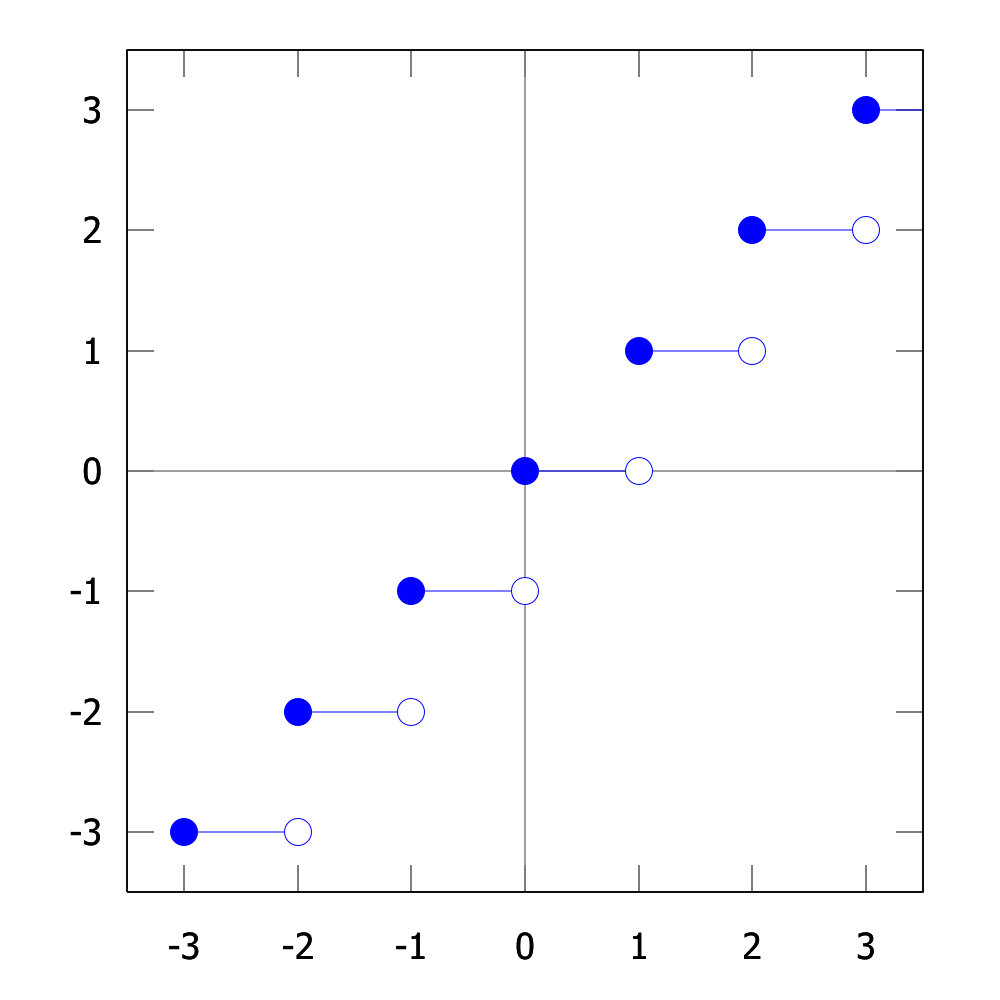
\includegraphics{figs/floor_function.png}

}

\caption{Fonction plancher}

}

\end{minipage}%
%
\begin{minipage}[t]{0.50\linewidth}

{\centering 

\raisebox{-\height}{

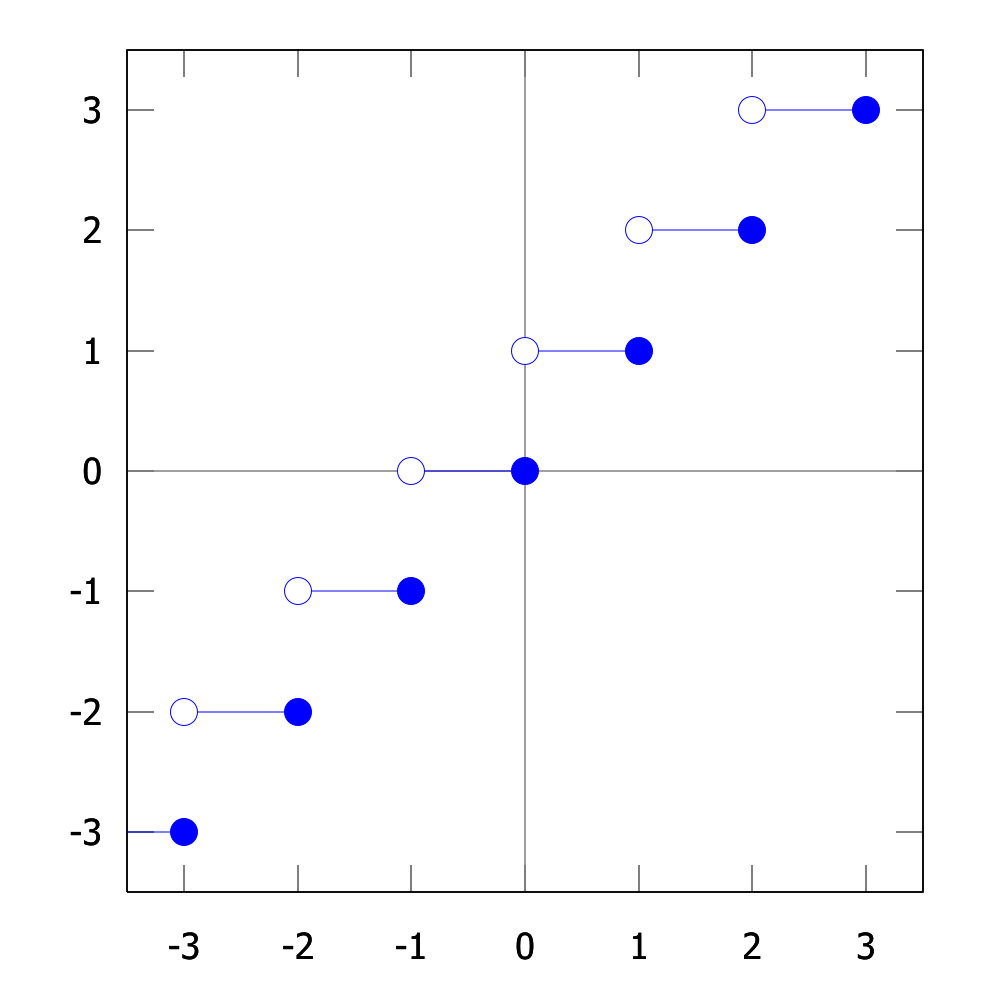
\includegraphics{figs/ceiling_function.png}

}

\caption{Fonction plafond}

}

\end{minipage}%

\caption{\label{fig-floor-ceiling}Les fonctions plancher et plafond.}

\end{figure}

Ces deux fonctions sont accessibles dans \texttt{Python} en utilisant la
librairie \texttt{math}, sous le nom de \texttt{floor} (\emph{fonction
plancher}) et \texttt{ceil} (\emph{fonction plafond}).

\hypertarget{fonctions-planchers-plafonds}{}
\begin{Shaded}
\begin{Highlighting}[]
\ImportTok{import}\NormalTok{ math}

\BuiltInTok{print}\NormalTok{(}\StringTok{"Résultats de la fonction plafond"}\NormalTok{)}
\BuiltInTok{print}\NormalTok{(math.ceil(}\FloatTok{1.4}\NormalTok{))}
\BuiltInTok{print}\NormalTok{(math.ceil(}\FloatTok{5.3}\NormalTok{))}
\BuiltInTok{print}\NormalTok{(math.ceil(}\OperatorTok{{-}}\FloatTok{5.3}\NormalTok{))}
\BuiltInTok{print}\NormalTok{(math.ceil(}\FloatTok{22.6}\NormalTok{))}
\BuiltInTok{print}\NormalTok{(math.ceil(}\FloatTok{10.0}\NormalTok{))}

\BuiltInTok{print}\NormalTok{(}\StringTok{"Résultats de la fonction plancher"}\NormalTok{)}
\BuiltInTok{print}\NormalTok{(math.floor(}\FloatTok{1.4}\NormalTok{))}
\BuiltInTok{print}\NormalTok{(math.floor(}\FloatTok{5.3}\NormalTok{))}
\BuiltInTok{print}\NormalTok{(math.floor(}\OperatorTok{{-}}\FloatTok{5.3}\NormalTok{))}
\BuiltInTok{print}\NormalTok{(math.floor(}\FloatTok{22.6}\NormalTok{))}
\BuiltInTok{print}\NormalTok{(math.floor(}\FloatTok{10.0}\NormalTok{))}
\end{Highlighting}
\end{Shaded}

\begin{verbatim}
Résultats de la fonction plafond
2
6
-5
23
10
Résultats de la fonction plancher
1
5
-6
22
10
\end{verbatim}

\hypertarget{fonctions-en-python}{%
\section{\texorpdfstring{Fonctions en
\texttt{Python}}{Fonctions en Python}}\label{fonctions-en-python}}

DEVRAIT-ON PARLER DE ÇA????

DICTIONNAIRE, HACHAGE\ldots{}

\begin{example}[]\protect\hypertarget{exm-hash-python}{}\label{exm-hash-python}

\href{https://www.wikiwand.com/en/Fowler\%E2\%80\%93Noll\%E2\%80\%93Vo_hash_function}{Fonction
de hachage dans Python}

\href{https://andrewbrookins.com/technology/pythons-default-hash-algorithm/}{Hachage
Python}

\href{https://thepythoncorner.com/posts/2020-08-21-hash-tables-understanding-dictionaries/}{Dictionnary
in Python}

A checksum is used to determine if something is the same.

If you have download a file, you can never be sure if it got corrupted
on the way to your machine. You can use cksum to calculate a checksum
(based on CRC-32) of the copy you now have and can then compare it to
the checksum the file should have. This is how you check for file
integrity.

A hash function is used to map data to other data of fixed size. A
perfect hash function is injective, so there are no collisions. Every
input has one fixed output.

A cryptographic hash function is used for verification. With a
cryptographic hash function you should to not be able to compute the
original input.

A very common use case is password hashing. This allows the verification
of a password without having to save the password itself. A service
provider only saves a hash of a password and is not able to compute the
original password. If the database of password hashes gets compromised,
an attacker should not be able to compute these passwords as well. This
is not the case, because there are strong and weak algorithms for
password hashing. You can find more on that on this very site.

TL;DR:

Checksums are used to compare two pieces of information to check if two
parties have exactly the same thing.

Hashes are used (in cryptography) to verify something, but this time,
deliberately only one party has access to the data that has to be
verified, while the other party only has access to the hash.

\end{example}

\hypertarget{injection-surjection-et-bijection}{%
\section{Injection, surjection et
bijection}\label{injection-surjection-et-bijection}}

\begin{definition}[Fonction injective, surjective,
bijective]\protect\hypertarget{def-fonction-injective-surjective-bijective}{}\label{def-fonction-injective-surjective-bijective}

Soit \(f:A\rightarrow B\) une fonction. On dit que

\begin{itemize}
\tightlist
\item
  \textbf{\(f\) est injective} si elle n'associe jamais la même image à
  deux éléments distincts: \[
  \forall\ a_1 \in A,\ \forall\ a_2 \in A,\ (a_1\neq a_2) \rightarrow (f(a_1) \neq f(a_2))
  \]
\item
  \textbf{\(f\) est surjective} si son image est l'ensemble \(B\) au
  complet, c'est-à-dire si tous les éléments de \(B\) sont atteints: \[
  \forall\ b\in B,\ \exists\ a \in A,\ f(a)=b
  \]
\item
  \textbf{\(f\) est bijective} si elle est injective et surjective: \[
  \forall\ b\in B,\ \exists! a\in A,\ f(a)=b
  \]
\end{itemize}

\end{definition}

\begin{tcolorbox}[enhanced jigsaw, colbacktitle=quarto-callout-important-color!10!white, toptitle=1mm, left=2mm, toprule=.15mm, opacityback=0, bottomrule=.15mm, breakable, coltitle=black, title=\textcolor{quarto-callout-important-color}{\faExclamation}\hspace{0.5em}{Important}, colframe=quarto-callout-important-color-frame, arc=.35mm, titlerule=0mm, rightrule=.15mm, opacitybacktitle=0.6, leftrule=.75mm, bottomtitle=1mm, colback=white]

Si une fonction n'est pas \textbf{injective}, alors elle ne possède pas
d'inverse.

\end{tcolorbox}

\begin{tcolorbox}[enhanced jigsaw, colbacktitle=quarto-callout-important-color!10!white, toptitle=1mm, left=2mm, toprule=.15mm, opacityback=0, bottomrule=.15mm, breakable, coltitle=black, title=\textcolor{quarto-callout-important-color}{\faExclamation}\hspace{0.5em}{Important}, colframe=quarto-callout-important-color-frame, arc=.35mm, titlerule=0mm, rightrule=.15mm, opacitybacktitle=0.6, leftrule=.75mm, bottomtitle=1mm, colback=white]

Si une fonction n'est pas \textbf{surjective}, alors elle ne possède pas
d'inverse.

\end{tcolorbox}

\begin{example}[]\protect\hypertarget{exm-fonction-injective-surjective-bijective}{}\label{exm-fonction-injective-surjective-bijective}

On considère un sous-ensemble \(f\) du produit cartésien de deux
ensembles. Dans chaque cas, tracez son graphe saggital puis déterminez
s'il s'agit d'une fonction ou non. De plus, si \(f\) est une fonction,
déterminez si elle est injective, surjective ou bijective.

Ici, \(L=\set{a,b,c,d,e}\), \(M=\set{a,b,c}\), \(C=\set{1,2,3,4}\) et
\(D=\set{1,2,3}\).

\begin{enumerate}
\def\labelenumi{\alph{enumi}.}
\tightlist
\item
  \(f=\set{(1,a),(2,d),(3,c),(4,e)}\subseteq C \times L\)
\item
  \(f=\set{(1,a),(2,a),(3,c),(4,b)}\subseteq C \times M\)
\item
  \(f=\set{(1,a),(2,d),(3,c),(4,e),(1,b)}\subseteq C \times L\)
\item
  \(f=\set{(1,c),(2,a),(3,a),(4,a)}\subseteq D \times M\)
\item
  \(f=\set{(1,a),(2,a),(3,a),(4,a)}\subseteq C \times L\)
\end{enumerate}

\end{example}

\begin{example}[]\protect\hypertarget{exm-fonction-dans-Z}{}\label{exm-fonction-dans-Z}

La fonction \(f:\mathbb{Z}\times\mathbb{Z}\rightarrow \mathbb{Z}\)
définie par \(f(x_1,x_2)=x_1+x^2\) est-elle oui on non injective?
Est-elle oui ou non surjective? Est-elle oui ou non bijective?

\end{example}

\hypertarget{les-dictionnaires-dans-python}{%
\subsection{\texorpdfstring{Les dictionnaires dans
\texttt{Python}}{Les dictionnaires dans Python}}\label{les-dictionnaires-dans-python}}

Le dictionnaire n'est pas une séquence mais un autre type composite. Ils
ressemblent aux listes dans une certaine mesure (ils sont modifiables
comme elles), mais les éléments que nous allons y enregistrer ne seront
pas disposés dans un ordre immuable. En revanche, nous pourrons accéder
à n'importe lequel d'entre eux à l'aide d'un index spécifique que l'on
appellera une clé, laquelle pourra être alphabétique, numérique, ou même
d'un type composite sous certaines conditions.

\begin{example}[]\protect\hypertarget{exm-jour-dejeuner-injective}{}\label{exm-jour-dejeuner-injective}

Dites si le dictionnaire défini ci-dessous est une fonction injective,
surjective, ou bijective.

\hypertarget{dictionnaries-days-breakfast-injective}{}
\begin{Shaded}
\begin{Highlighting}[]
\NormalTok{jour }\OperatorTok{=}\NormalTok{ \{}\StringTok{"Lundi"}\NormalTok{, }\StringTok{"Mardi"}\NormalTok{, }\StringTok{"Mercredi"}\NormalTok{, }\StringTok{"Jeudi"}\NormalTok{, }\StringTok{"Vendredi"}\NormalTok{, }\StringTok{"Samedi"}\NormalTok{, }\StringTok{"Dimanche"}\NormalTok{\}}
\NormalTok{dejeuner }\OperatorTok{=}\NormalTok{ \{}\StringTok{"Oeufs"}\NormalTok{, }\StringTok{"Céréales"}\NormalTok{, }\StringTok{"Rôties"}\NormalTok{, }\StringTok{"Gruau"}\NormalTok{, }\StringTok{"Pâtisserie"}\NormalTok{, }\StringTok{"Jambon"}\NormalTok{, }\StringTok{"Crèpes"}\NormalTok{,}\StringTok{"Saucisses"}\NormalTok{\}}

\NormalTok{mydict }\OperatorTok{=}\NormalTok{ \{}
    \StringTok{"Lundi"}\NormalTok{: }\StringTok{"Oeufs"}\NormalTok{,}
    \StringTok{"Mardi"}\NormalTok{: }\StringTok{"Céréales"}\NormalTok{,}
    \StringTok{"Mercredi"}\NormalTok{: }\StringTok{"Rôties"}\NormalTok{,}
    \StringTok{"Jeudi"}\NormalTok{: }\StringTok{"Gruau"}\NormalTok{,}
    \StringTok{"Vendredi"}\NormalTok{: }\StringTok{"Pâtisserie"}\NormalTok{,}
    \StringTok{"Samedi"}\NormalTok{: }\StringTok{"Jambon"}\NormalTok{,}
    \StringTok{"Dimanche"}\NormalTok{: }\StringTok{"Crèpes"}
\NormalTok{\}}
\end{Highlighting}
\end{Shaded}

\end{example}

\begin{example}[]\protect\hypertarget{exm-jour-dejeuner-non-injective}{}\label{exm-jour-dejeuner-non-injective}

Dites si le dictionnaire défini ci-dessous est une fonction injective,
surjective, ou bijective.

\hypertarget{dictionnaries-days-breakfast-non-injective}{}
\begin{Shaded}
\begin{Highlighting}[]
\NormalTok{jour }\OperatorTok{=}\NormalTok{ \{}\StringTok{"Lundi"}\NormalTok{, }\StringTok{"Mardi"}\NormalTok{, }\StringTok{"Mercredi"}\NormalTok{, }\StringTok{"Jeudi"}\NormalTok{, }\StringTok{"Vendredi"}\NormalTok{, }\StringTok{"Samedi"}\NormalTok{, }\StringTok{"Dimanche"}\NormalTok{\}}
\NormalTok{dejeuner }\OperatorTok{=}\NormalTok{ \{}\StringTok{"Oeufs"}\NormalTok{, }\StringTok{"Céréales"}\NormalTok{, }\StringTok{"Rôties"}\NormalTok{, }\StringTok{"Gruau"}\NormalTok{, }\StringTok{"Pâtisserie"}\NormalTok{, }\StringTok{"Jambon"}\NormalTok{, }\StringTok{"Crèpes"}\NormalTok{,}\StringTok{"Saucisses"}\NormalTok{\}}

\NormalTok{mydict }\OperatorTok{=}\NormalTok{ \{}
    \StringTok{"Lundi"}\NormalTok{: }\StringTok{"Oeufs"}\NormalTok{,}
    \StringTok{"Mardi"}\NormalTok{: }\StringTok{"Oeufs"}\NormalTok{,}
    \StringTok{"Mercredi"}\NormalTok{: }\StringTok{"Rôties"}\NormalTok{,}
    \StringTok{"Jeudi"}\NormalTok{: }\StringTok{"Gruau"}\NormalTok{,}
    \StringTok{"Vendredi"}\NormalTok{: }\StringTok{"Pâtisserie"}\NormalTok{,}
    \StringTok{"Samedi"}\NormalTok{: }\StringTok{"Jambon"}\NormalTok{,}
    \StringTok{"Dimanche"}\NormalTok{: }\StringTok{"Crèpes"}
\NormalTok{\}}
\end{Highlighting}
\end{Shaded}

\end{example}

\hypertarget{fonction-de-hachage}{%
\subsection{Fonction de hachage}\label{fonction-de-hachage}}

Une \textbf{fonction de hachage} est une fonction qui associe des
données de taille arbitraire à des valeurs de taille fixe. Les valeurs
renvoyées par une fonction de hachage sont appelées valeurs de hachage,
codes de hachage, résumés, signatures ou simplement hachages. Les
valeurs sont généralement utilisées pour être les indices d'une table de
taille raisonnable appelée table de hachage. Le hachage ou adressage de
stockage dispersé est donc l'utilisation d'une fonction de hachage pour
créer les indices d'une table de hachage.

Les fonctions de hachage sont utilisées dans les applications de
stockage et de récupération de données pour accéder aux données en un
temps réduit, en fait quasi-constant. Elles requièrent un espace de
stockage à peine plus grand que l'espace total requis pour les données.
Ainsi, le hachage est une forme d'accès aux données efficace en termes
de calcul et d'espace de stockage.

L'intérêt des fonctions de hachage repose sur de bonnes propriétés
statistiques. En effet, le comportement dans le pire des cas est
mauvais, mais il se manifeste avec une probabilité extrêmement faible,
en fait négligeable, et le comportement dans le cas moyen est optimal
(collision minimale ).

Une fonction de hachage est typiquement une fonction qui, pour un
ensemble de très grande taille (théoriquement infini) et de nature très
diversifiée, va renvoyer des résultats aux spécifications précises (en
général des chaînes de caractère de taille limitée ou fixe) optimisées
pour des applications particulières. Les chaînes permettent d'établir
des relations (égalité, égalité probable, non-égalité, ordre\ldots)
entre les objets de départ sans accéder directement à ces derniers, en
général soit pour des questions d'optimisation (la taille des objets de
départ nuit aux performances), soit pour des questions de
confidentialité.

Autrement dit : à 1 fichier (ou à 1 mot) va correspondre une signature
unique (le résultat de la fonction de hachage).

\begin{tcolorbox}[enhanced jigsaw, colbacktitle=quarto-callout-important-color!10!white, toptitle=1mm, left=2mm, toprule=.15mm, opacityback=0, bottomrule=.15mm, breakable, coltitle=black, title=\textcolor{quarto-callout-important-color}{\faExclamation}\hspace{0.5em}{Important}, colframe=quarto-callout-important-color-frame, arc=.35mm, titlerule=0mm, rightrule=.15mm, opacitybacktitle=0.6, leftrule=.75mm, bottomtitle=1mm, colback=white]

Dans l'idéal, une fonction de hachage \emph{devrait} être injective.

\end{tcolorbox}

On peut trouver le haché d'un élément en \texttt{Python} en utilisant la
commande \texttt{hash}. On peut remarquer dans le code ci-dessous que de
changer une lettre minuscule en lettre majuscule (le \emph{F} de
fromage) change drastiquement le haché.

\hypertarget{fonction-hachage-renard-corbeau}{}
\begin{Shaded}
\begin{Highlighting}[]
\NormalTok{phrase1 }\OperatorTok{=} \StringTok{"Maître Corbeau, sur un arbre perché, Tenait en son bec un fromage."}
\NormalTok{phrase2 }\OperatorTok{=} \StringTok{"Maître Corbeau, sur un arbre perché, Tenait en son bec un Fromage."}

\BuiltInTok{print}\NormalTok{(}\BuiltInTok{hex}\NormalTok{(}\BuiltInTok{hash}\NormalTok{(phrase1)), }\BuiltInTok{hex}\NormalTok{(}\BuiltInTok{hash}\NormalTok{(phrase2)))}
\end{Highlighting}
\end{Shaded}

\begin{verbatim}
-0x7998dd9b6ace271d -0x4f8bb80020376eb0
\end{verbatim}

\bookmarksetup{startatroot}

\hypertarget{notation-grand-o}{%
\chapter{Notation grand O}\label{notation-grand-o}}

\hypertarget{mesurer-un-temps-de-calcul-avec-une-fonction}{%
\section{Mesurer un temps de calcul avec une
fonction}\label{mesurer-un-temps-de-calcul-avec-une-fonction}}

\hypertarget{notation-grand-o-1}{%
\section{Notation grand-O}\label{notation-grand-o-1}}

\hypertarget{sommations}{%
\section{Sommations}\label{sommations}}

\hypertarget{uxe9tablir-la-complexituxe9-dun-algorithme}{%
\section{Établir la complexité d'un
algorithme}\label{uxe9tablir-la-complexituxe9-dun-algorithme}}

\hypertarget{calculabilituxe9-et-complexituxe9}{%
\section{Calculabilité et
complexité}\label{calculabilituxe9-et-complexituxe9}}

\hypertarget{p-vs-np}{%
\section{P vs NP}\label{p-vs-np}}

\bookmarksetup{startatroot}

\hypertarget{introduction-aux-algorithmes}{%
\chapter{Introduction aux
algorithmes}\label{introduction-aux-algorithmes}}

\hypertarget{bogo-sort}{%
\section{Bogo sort}\label{bogo-sort}}

\begin{Shaded}
\begin{Highlighting}[]
\ImportTok{from}\NormalTok{ random }\ImportTok{import}\NormalTok{ shuffle}
\ImportTok{from}\NormalTok{ random }\ImportTok{import}\NormalTok{ seed}
\ImportTok{from}\NormalTok{ random }\ImportTok{import}\NormalTok{ randint}

\KeywordTok{def}\NormalTok{ is\_sorted(data) }\OperatorTok{{-}\textgreater{}} \BuiltInTok{bool}\NormalTok{:}
    \CommentTok{"""Determine whether the data is sorted."""}
    \ControlFlowTok{return} \BuiltInTok{all}\NormalTok{(a }\OperatorTok{\textless{}=}\NormalTok{ b }\ControlFlowTok{for}\NormalTok{ a, b }\KeywordTok{in} \BuiltInTok{zip}\NormalTok{(data, data[}\DecValTok{1}\NormalTok{:]))}

\KeywordTok{def}\NormalTok{ bogosort(data) }\OperatorTok{{-}\textgreater{}} \BuiltInTok{list}\NormalTok{:}
    \CommentTok{"""Shuffle data until sorted."""}
\NormalTok{    N }\OperatorTok{=} \DecValTok{0}
    \ControlFlowTok{while} \KeywordTok{not}\NormalTok{ is\_sorted(data):}
\NormalTok{        shuffle(data)}
\NormalTok{        N }\OperatorTok{=}\NormalTok{ N }\OperatorTok{+} \DecValTok{1}
    \ControlFlowTok{return}\NormalTok{ data, N}

\NormalTok{seed(}\DecValTok{1234}\NormalTok{)}
\NormalTok{N }\OperatorTok{=} \DecValTok{8}
\NormalTok{data }\OperatorTok{=}\NormalTok{ [randint(}\DecValTok{1}\NormalTok{,}\DecValTok{10}\NormalTok{) }\ControlFlowTok{for}\NormalTok{ x }\KeywordTok{in} \BuiltInTok{range}\NormalTok{(N)]}
\NormalTok{bogosort(data)}
\end{Highlighting}
\end{Shaded}

\begin{verbatim}
([1, 1, 2, 2, 2, 2, 8, 10], 1552)
\end{verbatim}

\hypertarget{exemples-dalgorithmes}{%
\section{Exemples d'algorithmes}\label{exemples-dalgorithmes}}

\hypertarget{fouille-linuxe9aire}{%
\section{Fouille linéaire}\label{fouille-linuxe9aire}}

\hypertarget{bubble-sort}{%
\section{Bubble sort}\label{bubble-sort}}

\hypertarget{insertion-sort}{%
\section{Insertion sort}\label{insertion-sort}}

\hypertarget{binary-search}{%
\section{Binary search}\label{binary-search}}

\hypertarget{heap-sort}{%
\section{Heap sort}\label{heap-sort}}

\hypertarget{complexituxe9-algorithmique}{%
\section{Complexité algorithmique}\label{complexituxe9-algorithmique}}

\bookmarksetup{startatroot}

\hypertarget{thuxe9orie-des-nombres}{%
\chapter{Théorie des nombres}\label{thuxe9orie-des-nombres}}

\hypertarget{arithmuxe9tique-modulaire}{%
\section{Arithmétique modulaire}\label{arithmuxe9tique-modulaire}}

\hypertarget{division-entiuxe8re-1}{%
\subsection{Division entière}\label{division-entiuxe8re-1}}

\hypertarget{congruence-modulo-m}{%
\subsection{\texorpdfstring{Congruence modulo
\(m\)}{Congruence modulo m}}\label{congruence-modulo-m}}

\hypertarget{entiers-et-algorithmes}{%
\section{Entiers et algorithmes}\label{entiers-et-algorithmes}}

\hypertarget{algorithme-dexponentiation-modulaire-efficace}{%
\subsection{Algorithme d'exponentiation modulaire
efficace}\label{algorithme-dexponentiation-modulaire-efficace}}

\hypertarget{nombres-premiers-et-pgcd}{%
\subsection{Nombres premiers et PGCD}\label{nombres-premiers-et-pgcd}}

\hypertarget{algorithme-deuclide-et-thuxe9oruxe8me-de-buxe9zout}{%
\subsection{Algorithme d'Euclide et théorème de
Bézout}\label{algorithme-deuclide-et-thuxe9oruxe8me-de-buxe9zout}}

\hypertarget{inverse-modulo-m}{%
\subsection{\texorpdfstring{Inverse modulo
\(m\)}{Inverse modulo m}}\label{inverse-modulo-m}}

\hypertarget{ruxe9solution-de-congruence}{%
\subsection{Résolution de
congruence}\label{ruxe9solution-de-congruence}}

\hypertarget{petit-thuxe9oruxe8me-de-fermat}{%
\subsection{Petit théorème de
Fermat}\label{petit-thuxe9oruxe8me-de-fermat}}

\hypertarget{cryptographie-uxe0-cluxe9-secruxe8te}{%
\section{Cryptographie à clé
secrète}\label{cryptographie-uxe0-cluxe9-secruxe8te}}

\hypertarget{chiffrement-par-duxe9calage}{%
\subsection{Chiffrement par
décalage}\label{chiffrement-par-duxe9calage}}

\hypertarget{permutation-de-lalphabet}{%
\subsection{Permutation de l'alphabet}\label{permutation-de-lalphabet}}

\hypertarget{masque-jetable}{%
\subsection{Masque jetable}\label{masque-jetable}}

\hypertarget{chiffrement-affine}{%
\subsection{Chiffrement affine}\label{chiffrement-affine}}

\hypertarget{cryptographie-uxe0-cluxe9-publique}{%
\section{Cryptographie à clé
publique}\label{cryptographie-uxe0-cluxe9-publique}}

\hypertarget{chiffrement-rsa}{%
\subsection{Chiffrement RSA}\label{chiffrement-rsa}}

\bookmarksetup{startatroot}

\hypertarget{preuves-et-raisonnement-mathuxe9matique}{%
\chapter{Preuves et raisonnement
mathématique}\label{preuves-et-raisonnement-mathuxe9matique}}

\hypertarget{muxe9thodes-de-preuve}{%
\section{Méthodes de preuve}\label{muxe9thodes-de-preuve}}

\hypertarget{preuve-directe}{%
\subsection{Preuve directe}\label{preuve-directe}}

\begin{example}[]\protect\hypertarget{exm-produit-nombres-pairs-impairs}{}\label{exm-produit-nombres-pairs-impairs}

LE PRODUIT DE NOMBRES PAIRS ET IMPAIRS

\end{example}

\begin{example}[]\protect\hypertarget{exm-racines-nombres-pairs}{}\label{exm-racines-nombres-pairs}

RACINE DE NOMBRES PAIRS

\end{example}

\begin{example}[]\protect\hypertarget{exm-n2-pair}{}\label{exm-n2-pair}

PREUVE QUE \(n^2\) EST PAIR

\end{example}

\begin{example}[]\protect\hypertarget{exm-a-divise-b-divise-c}{}\label{exm-a-divise-b-divise-c}

Soit \(a\), \(b\) et \(c\) des entiers. Si \(a|b\) et \(b|c\) alors
\(a|c\).

\end{example}

\hypertarget{preuve-indirecte-par-contraposuxe9e}{%
\subsection{Preuve indirecte (par
contraposée)}\label{preuve-indirecte-par-contraposuxe9e}}

\begin{example}[]\protect\hypertarget{exm-n2-pair-alors-n-pair}{}\label{exm-n2-pair-alors-n-pair}

Montrez que si \(n^2\) est pair alors \(n\) est pair.

\end{example}

\begin{example}[]\protect\hypertarget{exm-aplusb-impair-a-b-impair}{}\label{exm-aplusb-impair-a-b-impair}

Montrez que si \(a+b\) est impair, alors \(a\) est impair ou \(b\) est
impair.

\end{example}

\begin{example}[]\protect\hypertarget{exm-nombre-premier-impair}{}\label{exm-nombre-premier-impair}

Soit \(p\) un nombre premier. Si \(p\neq 2\) alors \(p\) est impair.

\end{example}

\hypertarget{preuve-par-contradiction}{%
\subsection{Preuve par contradiction}\label{preuve-par-contradiction}}

\begin{example}[]\protect\hypertarget{exm-plus-petit-nombre-rationnel}{}\label{exm-plus-petit-nombre-rationnel}

EXISTE-T-IL UN PLUS PETIT NOMBRE RATIONNEL POSITIF?

\end{example}

\begin{example}[]\protect\hypertarget{exm-sqrt2-irrationnel}{}\label{exm-sqrt2-irrationnel}

PREUVE QUE \(\sqrt{2}\) EST IRRATIONNEL

\end{example}

\begin{example}[]\protect\hypertarget{exm-infinite-nombres-premiers}{}\label{exm-infinite-nombres-premiers}

PREUVE QUE QU'IL EXISTE UNE INFINITÉ DE NOMBRES PREMIERS

\end{example}

\begin{example}[]\protect\hypertarget{exm-pas-entiers-equation}{}\label{exm-pas-entiers-equation}

Il n'existe pas d'entiers \(x\) et \(y\) tels que \(x^2=4y+2\).

\end{example}

\hypertarget{principe-des-tiroirs-de-dirichlet}{%
\subsection{Principe des tiroirs de
Dirichlet}\label{principe-des-tiroirs-de-dirichlet}}

\begin{example}[Fonction de
hachage]\protect\hypertarget{exm-fonction-hachage}{}\label{exm-fonction-hachage}

Une fonction de hachage est une fonction qui transforme une suite de
bits de longueur arbitraire en une chaîne de longueur fixe. Du fait
qu'il y a plus de chaînes possibles en entrée qu'en sortie découle par
le principe des tiroirs l'existence de collisions : plusieurs chaînes
distinctes ont le même haché. Rendre ces collisions difficiles à
déterminer efficacement est un enjeu important en cryptographie.

\end{example}

\hypertarget{principe-de-linduction}{%
\section{Principe de l'induction}\label{principe-de-linduction}}

\hypertarget{preuve-par-ruxe9currence}{%
\subsection{Preuve par récurrence}\label{preuve-par-ruxe9currence}}

\begin{example}[]\protect\hypertarget{exm-somme-n-premiers-entiers}{}\label{exm-somme-n-premiers-entiers}

PREUVE QUE \(1+2+3+\ldots +n=\frac{n(n+1)}{2}\)

\end{example}

\begin{example}[]\protect\hypertarget{exm-n-plus-petit-2n}{}\label{exm-n-plus-petit-2n}

PREUVE QUE \(n<2^n\)

\end{example}

\begin{example}[]\protect\hypertarget{exm-6-divise-7n-1}{}\label{exm-6-divise-7n-1}

PREUVE QUE 6 EST UN DIVISEUR DE \(7^n-1\)

\end{example}

\begin{example}[]\protect\hypertarget{exm-space-filling-shapes}{}\label{exm-space-filling-shapes}

MONTRER QUE NOUS POUVONS UTILISER DES T-GONES POUR REMPLIR UNE GRILLE
\(2^n \times 2^n\)

\end{example}

\begin{example}[]\protect\hypertarget{exm-exponential-vs-factorial}{}\label{exm-exponential-vs-factorial}

MONTRER QUE LA FACTORIELLE CROÎT PLUS RAPIDEMENT QUE L'EXPONENTIELLE

\end{example}

\hypertarget{algorithmes-ruxe9cursifs}{%
\subsection{Algorithmes récursifs}\label{algorithmes-ruxe9cursifs}}

\hypertarget{fonctions-ruxe9cursives}{%
\subsubsection{Fonctions récursives}\label{fonctions-ruxe9cursives}}

\hypertarget{algorithmes-de-type-diviser-pour-ruxe9gner}{%
\subsubsection{Algorithmes de type diviser pour
régner}\label{algorithmes-de-type-diviser-pour-ruxe9gner}}

\bookmarksetup{startatroot}

\hypertarget{duxe9nombrement}{%
\chapter{Dénombrement}\label{duxe9nombrement}}

\hypertarget{notions-de-base}{%
\section{Notions de base}\label{notions-de-base}}

\hypertarget{principe-des-nids-de-pigeon-principe-des-tiroirs-de-dirichlet}{%
\section{Principe des nids de pigeon (principe des tiroirs de
Dirichlet)}\label{principe-des-nids-de-pigeon-principe-des-tiroirs-de-dirichlet}}

\hypertarget{permutations-et-combinaisons}{%
\section{Permutations et
combinaisons}\label{permutations-et-combinaisons}}

\hypertarget{relations-de-ruxe9currence-et-duxe9nombrement}{%
\section{Relations de récurrence et
dénombrement}\label{relations-de-ruxe9currence-et-duxe9nombrement}}

\bookmarksetup{startatroot}

\hypertarget{graphes}{%
\chapter{Graphes}\label{graphes}}

\hypertarget{terminologie-et-types-de-graphes}{%
\section{Terminologie et types de
graphes}\label{terminologie-et-types-de-graphes}}

\hypertarget{repruxe9sentation-des-graphes}{%
\section{Représentation des
graphes}\label{repruxe9sentation-des-graphes}}

\hypertarget{repruxe9sentation-par-listes-dadjacence}{%
\subsection{Représentation par listes
d'adjacence}\label{repruxe9sentation-par-listes-dadjacence}}

\hypertarget{repruxe9sentation-par-matrice-dadjacence}{%
\subsection{Représentation par matrice
d'adjacence}\label{repruxe9sentation-par-matrice-dadjacence}}

\hypertarget{chemins-dans-un-graphe}{%
\section{Chemins dans un graphe}\label{chemins-dans-un-graphe}}

\hypertarget{chemins-circuits-cycles}{%
\subsection{Chemins, circuits, cycles}\label{chemins-circuits-cycles}}

\hypertarget{duxe9nombrement-de-chemins}{%
\subsection{Dénombrement de chemins}\label{duxe9nombrement-de-chemins}}

\hypertarget{chemins-et-circuits-euluxe9riens}{%
\subsection{Chemins et circuits
eulériens}\label{chemins-et-circuits-euluxe9riens}}

\hypertarget{chemins-et-circuits-hamiltoniens}{%
\subsection{Chemins et circuits
hamiltoniens}\label{chemins-et-circuits-hamiltoniens}}

\hypertarget{probluxe8me-du-plus-court-chemin}{%
\section{Problème du plus court
chemin}\label{probluxe8me-du-plus-court-chemin}}

\bookmarksetup{startatroot}

\hypertarget{arbres}{%
\chapter{Arbres}\label{arbres}}

\hypertarget{introduction-aux-arbres}{%
\section{Introduction aux arbres}\label{introduction-aux-arbres}}

\hypertarget{applications-des-arbres}{%
\section{Applications des arbres}\label{applications-des-arbres}}

\hypertarget{parcours-dun-arbre}{%
\section{Parcours d'un arbre}\label{parcours-dun-arbre}}

\hypertarget{arbres-et-tri}{%
\section{Arbres et tri}\label{arbres-et-tri}}

\hypertarget{arbres-et-recouvrement}{%
\section{Arbres et recouvrement}\label{arbres-et-recouvrement}}

\hypertarget{arbres-guxe9nuxe9rateurs-de-couxfbt-minimal}{%
\section{Arbres générateurs de coût
minimal}\label{arbres-guxe9nuxe9rateurs-de-couxfbt-minimal}}

\bookmarksetup{startatroot}

\hypertarget{ruxe9fuxe9rences}{%
\chapter*{Références}\label{ruxe9fuxe9rences}}
\addcontentsline{toc}{chapter}{Références}

\markboth{Références}{Références}

\hypertarget{refs}{}
\begin{CSLReferences}{0}{0}
\end{CSLReferences}


\backmatter

\end{document}
